\documentclass{article}
\usepackage{iclr2027_conference,times}
\iclrfinalcopy
\usepackage[T1]{fontenc}
\usepackage[utf8]{inputenc}
\usepackage{amsmath,amssymb,graphicx,booktabs,longtable,array}
\usepackage{microtype,url,hyperref}
\hypersetup{pdftitle={Beyond Visual Token Count: Target Inclusion and Reader Recovery},pdfauthor={Goktug Aslanoglu and Viswanadh Vadlamani},pdfsubject={Preprint},colorlinks=true,linkcolor=blue,citecolor=blue,urlcolor=blue}
% Generated from audited machine-readable analysis; do not edit.
\newcommand{\nval}[1]{\csname n@#1\endcsname}
\expandafter\def\csname n@derived.layout.pairs\endcsname{144}
\expandafter\def\csname n@derived.rates.Qwen2B.optical_c0p8_p4.n\endcsname{180}
\expandafter\def\csname n@derived.rates.Qwen2B.optical_c0p8_p4.S\endcsname{7853}
\expandafter\def\csname n@derived.rates.Qwen2B.optical_c0p8_p4.V\endcsname{10000}
\expandafter\def\csname n@derived.rates.Qwen2B.optical_c0p8_p4.H\endcsname{81}
\expandafter\def\csname n@derived.rates.Qwen2B.optical_c0p8_p4.T\endcsname{10080}
\expandafter\def\csname n@derived.rates.Qwen2B.optical_c0p8_p4.Cmin\endcsname{0.784}
\expandafter\def\csname n@derived.rates.Qwen2B.optical_c0p8_p4.Cmed\endcsname{0.800}
\expandafter\def\csname n@derived.rates.Qwen2B.optical_c0p8_p4.Cmax\endcsname{0.816}
\expandafter\def\csname n@derived.rates.Qwen2B.optical_c2_p4.n\endcsname{180}
\expandafter\def\csname n@derived.rates.Qwen2B.optical_c2_p4.S\endcsname{7853}
\expandafter\def\csname n@derived.rates.Qwen2B.optical_c2_p4.V\endcsname{3844}
\expandafter\def\csname n@derived.rates.Qwen2B.optical_c2_p4.H\endcsname{81}
\expandafter\def\csname n@derived.rates.Qwen2B.optical_c2_p4.T\endcsname{4175}
\expandafter\def\csname n@derived.rates.Qwen2B.optical_c2_p4.Cmin\endcsname{1.952}
\expandafter\def\csname n@derived.rates.Qwen2B.optical_c2_p4.Cmed\endcsname{1.970}
\expandafter\def\csname n@derived.rates.Qwen2B.optical_c2_p4.Cmax\endcsname{2.064}
\expandafter\def\csname n@derived.rates.Qwen2B.optical_c4_p4.n\endcsname{180}
\expandafter\def\csname n@derived.rates.Qwen2B.optical_c4_p4.S\endcsname{7853}
\expandafter\def\csname n@derived.rates.Qwen2B.optical_c4_p4.V\endcsname{1936}
\expandafter\def\csname n@derived.rates.Qwen2B.optical_c4_p4.H\endcsname{81}
\expandafter\def\csname n@derived.rates.Qwen2B.optical_c4_p4.T\endcsname{2017}
\expandafter\def\csname n@derived.rates.Qwen2B.optical_c4_p4.Cmin\endcsname{3.828}
\expandafter\def\csname n@derived.rates.Qwen2B.optical_c4_p4.Cmed\endcsname{4.056}
\expandafter\def\csname n@derived.rates.Qwen2B.optical_c4_p4.Cmax\endcsname{4.134}
\expandafter\def\csname n@derived.budget.Qwen2B.long.gains\endcsname{5}
\expandafter\def\csname n@derived.budget.Qwen2B.long.losses\endcsname{7}
\expandafter\def\csname n@derived.incremental.Qwen2B.A_full_text.median\endcsname{0.935}
\expandafter\def\csname n@derived.incremental.Qwen2B.A_full_text.q25\endcsname{0.935}
\expandafter\def\csname n@derived.incremental.Qwen2B.A_full_text.q75\endcsname{0.935}
\expandafter\def\csname n@derived.incremental.Qwen2B.A_optical_C2.median\endcsname{0.733}
\expandafter\def\csname n@derived.incremental.Qwen2B.A_optical_C2.q25\endcsname{0.733}
\expandafter\def\csname n@derived.incremental.Qwen2B.A_optical_C2.q75\endcsname{0.733}
\expandafter\def\csname n@derived.incremental.Qwen2B.A_optical_C4.median\endcsname{0.385}
\expandafter\def\csname n@derived.incremental.Qwen2B.A_optical_C4.q25\endcsname{0.385}
\expandafter\def\csname n@derived.incremental.Qwen2B.A_optical_C4.q75\endcsname{0.385}
\expandafter\def\csname n@derived.incremental.Qwen2B.B_text.median\endcsname{0.486}
\expandafter\def\csname n@derived.incremental.Qwen2B.B_text.q25\endcsname{0.486}
\expandafter\def\csname n@derived.incremental.Qwen2B.B_text.q75\endcsname{0.486}
\expandafter\def\csname n@derived.incremental.Qwen2B.B_optical.median\endcsname{0.733}
\expandafter\def\csname n@derived.incremental.Qwen2B.B_optical.q25\endcsname{0.733}
\expandafter\def\csname n@derived.incremental.Qwen2B.B_optical.q75\endcsname{0.733}
\expandafter\def\csname n@derived.rates.Qwen9B.optical_c0p8_p4.n\endcsname{180}
\expandafter\def\csname n@derived.rates.Qwen9B.optical_c0p8_p4.S\endcsname{7853}
\expandafter\def\csname n@derived.rates.Qwen9B.optical_c0p8_p4.V\endcsname{10000}
\expandafter\def\csname n@derived.rates.Qwen9B.optical_c0p8_p4.H\endcsname{81}
\expandafter\def\csname n@derived.rates.Qwen9B.optical_c0p8_p4.T\endcsname{10080}
\expandafter\def\csname n@derived.rates.Qwen9B.optical_c0p8_p4.Cmin\endcsname{0.784}
\expandafter\def\csname n@derived.rates.Qwen9B.optical_c0p8_p4.Cmed\endcsname{0.800}
\expandafter\def\csname n@derived.rates.Qwen9B.optical_c0p8_p4.Cmax\endcsname{0.816}
\expandafter\def\csname n@derived.rates.Qwen9B.optical_c2_p4.n\endcsname{180}
\expandafter\def\csname n@derived.rates.Qwen9B.optical_c2_p4.S\endcsname{7853}
\expandafter\def\csname n@derived.rates.Qwen9B.optical_c2_p4.V\endcsname{3844}
\expandafter\def\csname n@derived.rates.Qwen9B.optical_c2_p4.H\endcsname{81}
\expandafter\def\csname n@derived.rates.Qwen9B.optical_c2_p4.T\endcsname{4175}
\expandafter\def\csname n@derived.rates.Qwen9B.optical_c2_p4.Cmin\endcsname{1.952}
\expandafter\def\csname n@derived.rates.Qwen9B.optical_c2_p4.Cmed\endcsname{1.970}
\expandafter\def\csname n@derived.rates.Qwen9B.optical_c2_p4.Cmax\endcsname{2.064}
\expandafter\def\csname n@derived.rates.Qwen9B.optical_c4_p4.n\endcsname{180}
\expandafter\def\csname n@derived.rates.Qwen9B.optical_c4_p4.S\endcsname{7853}
\expandafter\def\csname n@derived.rates.Qwen9B.optical_c4_p4.V\endcsname{1936}
\expandafter\def\csname n@derived.rates.Qwen9B.optical_c4_p4.H\endcsname{81}
\expandafter\def\csname n@derived.rates.Qwen9B.optical_c4_p4.T\endcsname{2017}
\expandafter\def\csname n@derived.rates.Qwen9B.optical_c4_p4.Cmin\endcsname{3.828}
\expandafter\def\csname n@derived.rates.Qwen9B.optical_c4_p4.Cmed\endcsname{4.056}
\expandafter\def\csname n@derived.rates.Qwen9B.optical_c4_p4.Cmax\endcsname{4.134}
\expandafter\def\csname n@derived.budget.Qwen9B.long.gains\endcsname{8}
\expandafter\def\csname n@derived.budget.Qwen9B.long.losses\endcsname{4}
\expandafter\def\csname n@derived.incremental.Qwen9B.A_full_text.median\endcsname{1.990}
\expandafter\def\csname n@derived.incremental.Qwen9B.A_full_text.q25\endcsname{1.990}
\expandafter\def\csname n@derived.incremental.Qwen9B.A_full_text.q75\endcsname{1.990}
\expandafter\def\csname n@derived.incremental.Qwen9B.A_optical_C2.median\endcsname{1.225}
\expandafter\def\csname n@derived.incremental.Qwen9B.A_optical_C2.q25\endcsname{1.225}
\expandafter\def\csname n@derived.incremental.Qwen9B.A_optical_C2.q75\endcsname{1.225}
\expandafter\def\csname n@derived.incremental.Qwen9B.A_optical_C4.median\endcsname{0.674}
\expandafter\def\csname n@derived.incremental.Qwen9B.A_optical_C4.q25\endcsname{0.674}
\expandafter\def\csname n@derived.incremental.Qwen9B.A_optical_C4.q75\endcsname{0.674}
\expandafter\def\csname n@derived.incremental.Qwen9B.B_text.median\endcsname{1.034}
\expandafter\def\csname n@derived.incremental.Qwen9B.B_text.q25\endcsname{1.034}
\expandafter\def\csname n@derived.incremental.Qwen9B.B_text.q75\endcsname{1.034}
\expandafter\def\csname n@derived.incremental.Qwen9B.B_optical.median\endcsname{1.225}
\expandafter\def\csname n@derived.incremental.Qwen9B.B_optical.q25\endcsname{1.225}
\expandafter\def\csname n@derived.incremental.Qwen9B.B_optical.q75\endcsname{1.225}
\expandafter\def\csname n@derived.rates.GLM.optical_c0p8_p4.n\endcsname{180}
\expandafter\def\csname n@derived.rates.GLM.optical_c0p8_p4.S\endcsname{7387}
\expandafter\def\csname n@derived.rates.GLM.optical_c0p8_p4.V\endcsname{9216}
\expandafter\def\csname n@derived.rates.GLM.optical_c0p8_p4.H\endcsname{78}
\expandafter\def\csname n@derived.rates.GLM.optical_c0p8_p4.T\endcsname{9682}
\expandafter\def\csname n@derived.rates.GLM.optical_c0p8_p4.Cmin\endcsname{0.787}
\expandafter\def\csname n@derived.rates.GLM.optical_c0p8_p4.Cmed\endcsname{0.797}
\expandafter\def\csname n@derived.rates.GLM.optical_c0p8_p4.Cmax\endcsname{0.802}
\expandafter\def\csname n@derived.rates.GLM.optical_c2_p4.n\endcsname{180}
\expandafter\def\csname n@derived.rates.GLM.optical_c2_p4.S\endcsname{7387}
\expandafter\def\csname n@derived.rates.GLM.optical_c2_p4.V\endcsname{3600}
\expandafter\def\csname n@derived.rates.GLM.optical_c2_p4.H\endcsname{78}
\expandafter\def\csname n@derived.rates.GLM.optical_c2_p4.T\endcsname{3922}
\expandafter\def\csname n@derived.rates.GLM.optical_c2_p4.Cmin\endcsname{1.944}
\expandafter\def\csname n@derived.rates.GLM.optical_c2_p4.Cmed\endcsname{2.020}
\expandafter\def\csname n@derived.rates.GLM.optical_c2_p4.Cmax\endcsname{2.070}
\expandafter\def\csname n@derived.rates.GLM.optical_c4_p4.n\endcsname{180}
\expandafter\def\csname n@derived.rates.GLM.optical_c4_p4.S\endcsname{7387}
\expandafter\def\csname n@derived.rates.GLM.optical_c4_p4.V\endcsname{1936}
\expandafter\def\csname n@derived.rates.GLM.optical_c4_p4.H\endcsname{78}
\expandafter\def\csname n@derived.rates.GLM.optical_c4_p4.T\endcsname{2012}
\expandafter\def\csname n@derived.rates.GLM.optical_c4_p4.Cmin\endcsname{3.815}
\expandafter\def\csname n@derived.rates.GLM.optical_c4_p4.Cmed\endcsname{4.115}
\expandafter\def\csname n@derived.rates.GLM.optical_c4_p4.Cmax\endcsname{4.186}
\expandafter\def\csname n@derived.budget.GLM.long.gains\endcsname{10}
\expandafter\def\csname n@derived.budget.GLM.long.losses\endcsname{1}
\expandafter\def\csname n@derived.incremental.GLM.A_full_text.median\endcsname{1.229}
\expandafter\def\csname n@derived.incremental.GLM.A_full_text.q25\endcsname{1.229}
\expandafter\def\csname n@derived.incremental.GLM.A_full_text.q75\endcsname{1.229}
\expandafter\def\csname n@derived.incremental.GLM.A_optical_C2.median\endcsname{0.847}
\expandafter\def\csname n@derived.incremental.GLM.A_optical_C2.q25\endcsname{0.847}
\expandafter\def\csname n@derived.incremental.GLM.A_optical_C2.q75\endcsname{0.847}
\expandafter\def\csname n@derived.incremental.GLM.A_optical_C4.median\endcsname{0.420}
\expandafter\def\csname n@derived.incremental.GLM.A_optical_C4.q25\endcsname{0.420}
\expandafter\def\csname n@derived.incremental.GLM.A_optical_C4.q75\endcsname{0.420}
\expandafter\def\csname n@derived.incremental.GLM.B_text.median\endcsname{0.672}
\expandafter\def\csname n@derived.incremental.GLM.B_text.q25\endcsname{0.672}
\expandafter\def\csname n@derived.incremental.GLM.B_text.q75\endcsname{0.672}
\expandafter\def\csname n@derived.incremental.GLM.B_optical.median\endcsname{0.906}
\expandafter\def\csname n@derived.incremental.GLM.B_optical.q25\endcsname{0.906}
\expandafter\def\csname n@derived.incremental.GLM.B_optical.q75\endcsname{0.906}
\expandafter\def\csname n@loc.Qwen2B.full_optical_c2.conversation_macro_f1\endcsname{9.84}
\expandafter\def\csname n@loc.Qwen2B.full_optical_c2.question_micro_f1\endcsname{9.26}
\expandafter\def\csname n@loc.Qwen2B.full_optical_c2.mean_input_tokens\endcsname{20081.75}
\expandafter\def\csname n@loc.Qwen2B.full_optical_c2.cap\endcsname{126}
\expandafter\def\csname n@loc.Qwen2B.full_raw.conversation_macro_f1\endcsname{48.45}
\expandafter\def\csname n@loc.Qwen2B.full_raw.question_micro_f1\endcsname{48.55}
\expandafter\def\csname n@loc.Qwen2B.full_raw.mean_input_tokens\endcsname{39713.18}
\expandafter\def\csname n@loc.Qwen2B.full_raw.cap\endcsname{14}
\expandafter\def\csname n@loc.Qwen2B.retrieved_optical_8px.conversation_macro_f1\endcsname{28.89}
\expandafter\def\csname n@loc.Qwen2B.retrieved_optical_8px.question_micro_f1\endcsname{28.98}
\expandafter\def\csname n@loc.Qwen2B.retrieved_optical_8px.mean_input_tokens\endcsname{1913.24}
\expandafter\def\csname n@loc.Qwen2B.retrieved_optical_8px.cap\endcsname{2}
\expandafter\def\csname n@loc.Qwen2B.retrieved_text.conversation_macro_f1\endcsname{39.98}
\expandafter\def\csname n@loc.Qwen2B.retrieved_text.question_micro_f1\endcsname{40.15}
\expandafter\def\csname n@loc.Qwen2B.retrieved_text.mean_input_tokens\endcsname{1185.19}
\expandafter\def\csname n@loc.Qwen2B.retrieved_text.cap\endcsname{0}
\expandafter\def\csname n@loc.Qwen2B.retrieved_text_matched.conversation_macro_f1\endcsname{48.34}
\expandafter\def\csname n@loc.Qwen2B.retrieved_text_matched.question_micro_f1\endcsname{48.67}
\expandafter\def\csname n@loc.Qwen2B.retrieved_text_matched.mean_input_tokens\endcsname{20069.56}
\expandafter\def\csname n@loc.Qwen2B.retrieved_text_matched.cap\endcsname{13}
\expandafter\def\csname n@loc.Qwen2B.retrieved_text_matched_selected.conversation_macro_f1\endcsname{40.74}
\expandafter\def\csname n@loc.Qwen2B.retrieved_text_matched_selected.question_micro_f1\endcsname{41.14}
\expandafter\def\csname n@loc.Qwen2B.retrieved_text_matched_selected.mean_input_tokens\endcsname{1872.24}
\expandafter\def\csname n@loc.Qwen2B.retrieved_text_matched_selected.cap\endcsname{0}
\expandafter\def\csname n@loc.Qwen2B.H1.effect\endcsname{19.05}
\expandafter\def\csname n@loc.Qwen2B.H1.lo\endcsname{15.79}
\expandafter\def\csname n@loc.Qwen2B.H1.hi\endcsname{22.46}
\expandafter\def\csname n@loc.Qwen2B.H2.effect\endcsname{-11.09}
\expandafter\def\csname n@loc.Qwen2B.H2.lo\endcsname{-14.08}
\expandafter\def\csname n@loc.Qwen2B.H2.hi\endcsname{-8.27}
\expandafter\def\csname n@loc.Qwen2B.selected_budget.effect\endcsname{-11.85}
\expandafter\def\csname n@loc.Qwen2B.selected_budget.lo\endcsname{-15.70}
\expandafter\def\csname n@loc.Qwen2B.selected_budget.hi\endcsname{-8.58}
\expandafter\def\csname n@loc.Qwen2B.full_budget.effect\endcsname{-38.51}
\expandafter\def\csname n@loc.Qwen2B.full_budget.lo\endcsname{-41.61}
\expandafter\def\csname n@loc.Qwen2B.full_budget.hi\endcsname{-35.18}
\expandafter\def\csname n@loc.Qwen2B.full_raw_gap.effect\endcsname{38.61}
\expandafter\def\csname n@loc.Qwen2B.full_raw_gap.lo\endcsname{35.47}
\expandafter\def\csname n@loc.Qwen2B.full_raw_gap.hi\endcsname{41.28}
\expandafter\def\csname n@ruler.Qwen2B.full_raw\endcsname{90.64}
\expandafter\def\csname n@ruler.Qwen2B.optical_c0p8_p4\endcsname{74.56}
\expandafter\def\csname n@ruler.Qwen2B.optical_c2_p4\endcsname{46.11}
\expandafter\def\csname n@ruler.Qwen2B.optical_c4_p4\endcsname{5.44}
\expandafter\def\csname n@id.Qwen2B.full_raw\endcsname{90}
\expandafter\def\csname n@id.Qwen2B.optical_c0p8_p2\endcsname{0}
\expandafter\def\csname n@id.Qwen2B.optical_c0p8_p4\endcsname{13}
\expandafter\def\csname n@id.Qwen2B.optical_c2_p2\endcsname{0}
\expandafter\def\csname n@id.Qwen2B.optical_c2_p4\endcsname{0}
\expandafter\def\csname n@id.Qwen2B.optical_c4_p2\endcsname{0}
\expandafter\def\csname n@id.Qwen2B.optical_c4_p4\endcsname{0}
\expandafter\def\csname n@layout.Qwen2B.full_raw\endcsname{47}
\expandafter\def\csname n@layout.Qwen2B.original_c2_p4\endcsname{0}
\expandafter\def\csname n@layout.Qwen2B.efficient_c2_p4\endcsname{6}
\expandafter\def\csname n@layout.Qwen2B.readable_p4\endcsname{17}
\expandafter\def\csname n@layout.Qwen2B.effect\endcsname{12.50}
\expandafter\def\csname n@layout.Qwen2B.lo\endcsname{6.25}
\expandafter\def\csname n@layout.Qwen2B.hi\endcsname{18.75}
\expandafter\def\csname n@layout.Qwen2B.p\endcsname{0.03125}
\expandafter\def\csname n@layout.Qwen2B.holm\endcsname{0.03125}
\expandafter\def\csname n@layout.Qwen2B.gain\endcsname{6}
\expandafter\def\csname n@layout.Qwen2B.loss\endcsname{0}
\expandafter\def\csname n@budget.Qwen2B.short.text\endcsname{30}
\expandafter\def\csname n@budget.Qwen2B.short.optical\endcsname{27}
\expandafter\def\csname n@budget.Qwen2B.short.effect\endcsname{-10.00}
\expandafter\def\csname n@budget.Qwen2B.short.lo\endcsname{-23.33}
\expandafter\def\csname n@budget.Qwen2B.short.hi\endcsname{0.00}
\expandafter\def\csname n@budget.Qwen2B.medium.text\endcsname{22}
\expandafter\def\csname n@budget.Qwen2B.medium.optical\endcsname{22}
\expandafter\def\csname n@budget.Qwen2B.medium.effect\endcsname{0.00}
\expandafter\def\csname n@budget.Qwen2B.medium.lo\endcsname{-23.33}
\expandafter\def\csname n@budget.Qwen2B.medium.hi\endcsname{23.33}
\expandafter\def\csname n@budget.Qwen2B.long.text\endcsname{18}
\expandafter\def\csname n@budget.Qwen2B.long.optical\endcsname{16}
\expandafter\def\csname n@budget.Qwen2B.long.effect\endcsname{-6.67}
\expandafter\def\csname n@budget.Qwen2B.long.lo\endcsname{-30.00}
\expandafter\def\csname n@budget.Qwen2B.long.hi\endcsname{16.67}
\expandafter\def\csname n@budget.Qwen2B.primary_interaction.effect\endcsname{3.33}
\expandafter\def\csname n@budget.Qwen2B.primary_interaction.lo\endcsname{-20.00}
\expandafter\def\csname n@budget.Qwen2B.primary_interaction.hi\endcsname{26.67}
\expandafter\def\csname n@budget.Qwen2B.primary_interaction.holm\endcsname{1.0000}
\expandafter\def\csname n@budget.Qwen2B.secondary_long.effect\endcsname{-6.67}
\expandafter\def\csname n@budget.Qwen2B.secondary_long.lo\endcsname{-30.00}
\expandafter\def\csname n@budget.Qwen2B.secondary_long.hi\endcsname{16.67}
\expandafter\def\csname n@budget.Qwen2B.secondary_long.holm\endcsname{0.7754}
\expandafter\def\csname n@scale.Qwen2B.0.55.correct\endcsname{0}
\expandafter\def\csname n@scale.Qwen2B.0.55.cer\endcsname{1.962}
\expandafter\def\csname n@scale.Qwen2B.0.55.cap_hits\endcsname{4}
\expandafter\def\csname n@scale.Qwen2B.0.75.correct\endcsname{3}
\expandafter\def\csname n@scale.Qwen2B.0.75.cer\endcsname{1.132}
\expandafter\def\csname n@scale.Qwen2B.0.75.cap_hits\endcsname{1}
\expandafter\def\csname n@scale.Qwen2B.1.00.correct\endcsname{2}
\expandafter\def\csname n@scale.Qwen2B.1.00.cer\endcsname{1.260}
\expandafter\def\csname n@scale.Qwen2B.1.00.cap_hits\endcsname{2}
\expandafter\def\csname n@scale.Qwen2B.holm\endcsname{0.2588}
\expandafter\def\csname n@scale.Qwen2B.Q\endcsname{4.6667}
\expandafter\def\csname n@scale.Qwen2B.0.effect\endcsname{6.250}
\expandafter\def\csname n@scale.Qwen2B.0.lo\endcsname{0.000}
\expandafter\def\csname n@scale.Qwen2B.0.hi\endcsname{15.625}
\expandafter\def\csname n@scale.Qwen2B.0.p\endcsname{0.500000}
\expandafter\def\csname n@scale.Qwen2B.0.holm\endcsname{1.000000}
\expandafter\def\csname n@scale.Qwen2B.0.gains\endcsname{2}
\expandafter\def\csname n@scale.Qwen2B.0.losses\endcsname{0}
\expandafter\def\csname n@scale.Qwen2B.1.effect\endcsname{-3.125}
\expandafter\def\csname n@scale.Qwen2B.1.lo\endcsname{-9.375}
\expandafter\def\csname n@scale.Qwen2B.1.hi\endcsname{0.000}
\expandafter\def\csname n@scale.Qwen2B.1.p\endcsname{1.000000}
\expandafter\def\csname n@scale.Qwen2B.1.holm\endcsname{1.000000}
\expandafter\def\csname n@scale.Qwen2B.1.gains\endcsname{0}
\expandafter\def\csname n@scale.Qwen2B.1.losses\endcsname{1}
\expandafter\def\csname n@scale.Qwen2B.2.effect\endcsname{9.375}
\expandafter\def\csname n@scale.Qwen2B.2.lo\endcsname{0.000}
\expandafter\def\csname n@scale.Qwen2B.2.hi\endcsname{21.875}
\expandafter\def\csname n@scale.Qwen2B.2.p\endcsname{0.250000}
\expandafter\def\csname n@scale.Qwen2B.2.holm\endcsname{1.000000}
\expandafter\def\csname n@scale.Qwen2B.2.gains\endcsname{3}
\expandafter\def\csname n@scale.Qwen2B.2.losses\endcsname{0}
\expandafter\def\csname n@loc.Qwen9B.full_optical_c2.conversation_macro_f1\endcsname{15.95}
\expandafter\def\csname n@loc.Qwen9B.full_optical_c2.question_micro_f1\endcsname{15.21}
\expandafter\def\csname n@loc.Qwen9B.full_optical_c2.mean_input_tokens\endcsname{20081.75}
\expandafter\def\csname n@loc.Qwen9B.full_optical_c2.cap\endcsname{121}
\expandafter\def\csname n@loc.Qwen9B.full_raw.conversation_macro_f1\endcsname{53.04}
\expandafter\def\csname n@loc.Qwen9B.full_raw.question_micro_f1\endcsname{52.44}
\expandafter\def\csname n@loc.Qwen9B.full_raw.mean_input_tokens\endcsname{39713.18}
\expandafter\def\csname n@loc.Qwen9B.full_raw.cap\endcsname{12}
\expandafter\def\csname n@loc.Qwen9B.retrieved_optical_8px.conversation_macro_f1\endcsname{35.28}
\expandafter\def\csname n@loc.Qwen9B.retrieved_optical_8px.question_micro_f1\endcsname{35.70}
\expandafter\def\csname n@loc.Qwen9B.retrieved_optical_8px.mean_input_tokens\endcsname{1913.24}
\expandafter\def\csname n@loc.Qwen9B.retrieved_optical_8px.cap\endcsname{0}
\expandafter\def\csname n@loc.Qwen9B.retrieved_text.conversation_macro_f1\endcsname{37.22}
\expandafter\def\csname n@loc.Qwen9B.retrieved_text.question_micro_f1\endcsname{37.76}
\expandafter\def\csname n@loc.Qwen9B.retrieved_text.mean_input_tokens\endcsname{1185.19}
\expandafter\def\csname n@loc.Qwen9B.retrieved_text.cap\endcsname{2}
\expandafter\def\csname n@loc.Qwen9B.retrieved_text_matched.conversation_macro_f1\endcsname{49.77}
\expandafter\def\csname n@loc.Qwen9B.retrieved_text_matched.question_micro_f1\endcsname{49.71}
\expandafter\def\csname n@loc.Qwen9B.retrieved_text_matched.mean_input_tokens\endcsname{20069.56}
\expandafter\def\csname n@loc.Qwen9B.retrieved_text_matched.cap\endcsname{8}
\expandafter\def\csname n@loc.Qwen9B.retrieved_text_matched_selected.conversation_macro_f1\endcsname{39.11}
\expandafter\def\csname n@loc.Qwen9B.retrieved_text_matched_selected.question_micro_f1\endcsname{39.59}
\expandafter\def\csname n@loc.Qwen9B.retrieved_text_matched_selected.mean_input_tokens\endcsname{1872.24}
\expandafter\def\csname n@loc.Qwen9B.retrieved_text_matched_selected.cap\endcsname{1}
\expandafter\def\csname n@loc.Qwen9B.H1.effect\endcsname{19.33}
\expandafter\def\csname n@loc.Qwen9B.H1.lo\endcsname{14.99}
\expandafter\def\csname n@loc.Qwen9B.H1.hi\endcsname{22.97}
\expandafter\def\csname n@loc.Qwen9B.H2.effect\endcsname{-1.94}
\expandafter\def\csname n@loc.Qwen9B.H2.lo\endcsname{-3.76}
\expandafter\def\csname n@loc.Qwen9B.H2.hi\endcsname{-0.13}
\expandafter\def\csname n@loc.Qwen9B.selected_budget.effect\endcsname{-3.83}
\expandafter\def\csname n@loc.Qwen9B.selected_budget.lo\endcsname{-4.69}
\expandafter\def\csname n@loc.Qwen9B.selected_budget.hi\endcsname{-3.10}
\expandafter\def\csname n@loc.Qwen9B.full_budget.effect\endcsname{-33.81}
\expandafter\def\csname n@loc.Qwen9B.full_budget.lo\endcsname{-37.73}
\expandafter\def\csname n@loc.Qwen9B.full_budget.hi\endcsname{-29.94}
\expandafter\def\csname n@loc.Qwen9B.full_raw_gap.effect\endcsname{37.09}
\expandafter\def\csname n@loc.Qwen9B.full_raw_gap.lo\endcsname{33.82}
\expandafter\def\csname n@loc.Qwen9B.full_raw_gap.hi\endcsname{40.59}
\expandafter\def\csname n@ruler.Qwen9B.full_raw\endcsname{99.17}
\expandafter\def\csname n@ruler.Qwen9B.optical_c0p8_p4\endcsname{83.72}
\expandafter\def\csname n@ruler.Qwen9B.optical_c2_p4\endcsname{55.64}
\expandafter\def\csname n@ruler.Qwen9B.optical_c4_p4\endcsname{8.06}
\expandafter\def\csname n@id.Qwen9B.full_raw\endcsname{93}
\expandafter\def\csname n@id.Qwen9B.optical_c0p8_p2\endcsname{3}
\expandafter\def\csname n@id.Qwen9B.optical_c0p8_p4\endcsname{22}
\expandafter\def\csname n@id.Qwen9B.optical_c2_p2\endcsname{0}
\expandafter\def\csname n@id.Qwen9B.optical_c2_p4\endcsname{0}
\expandafter\def\csname n@id.Qwen9B.optical_c4_p2\endcsname{0}
\expandafter\def\csname n@id.Qwen9B.optical_c4_p4\endcsname{0}
\expandafter\def\csname n@layout.Qwen9B.full_raw\endcsname{46}
\expandafter\def\csname n@layout.Qwen9B.original_c2_p4\endcsname{0}
\expandafter\def\csname n@layout.Qwen9B.efficient_c2_p4\endcsname{21}
\expandafter\def\csname n@layout.Qwen9B.readable_p4\endcsname{35}
\expandafter\def\csname n@layout.Qwen9B.effect\endcsname{43.75}
\expandafter\def\csname n@layout.Qwen9B.lo\endcsname{35.42}
\expandafter\def\csname n@layout.Qwen9B.hi\endcsname{52.08}
\expandafter\def\csname n@layout.Qwen9B.p\endcsname{9.53674e-07}
\expandafter\def\csname n@layout.Qwen9B.holm\endcsname{2.86102e-06}
\expandafter\def\csname n@layout.Qwen9B.gain\endcsname{21}
\expandafter\def\csname n@layout.Qwen9B.loss\endcsname{0}
\expandafter\def\csname n@budget.Qwen9B.short.text\endcsname{30}
\expandafter\def\csname n@budget.Qwen9B.short.optical\endcsname{30}
\expandafter\def\csname n@budget.Qwen9B.short.effect\endcsname{0.00}
\expandafter\def\csname n@budget.Qwen9B.short.lo\endcsname{0.00}
\expandafter\def\csname n@budget.Qwen9B.short.hi\endcsname{0.00}
\expandafter\def\csname n@budget.Qwen9B.medium.text\endcsname{22}
\expandafter\def\csname n@budget.Qwen9B.medium.optical\endcsname{27}
\expandafter\def\csname n@budget.Qwen9B.medium.effect\endcsname{16.67}
\expandafter\def\csname n@budget.Qwen9B.medium.lo\endcsname{-3.33}
\expandafter\def\csname n@budget.Qwen9B.medium.hi\endcsname{36.67}
\expandafter\def\csname n@budget.Qwen9B.long.text\endcsname{18}
\expandafter\def\csname n@budget.Qwen9B.long.optical\endcsname{22}
\expandafter\def\csname n@budget.Qwen9B.long.effect\endcsname{13.33}
\expandafter\def\csname n@budget.Qwen9B.long.lo\endcsname{-10.00}
\expandafter\def\csname n@budget.Qwen9B.long.hi\endcsname{36.67}
\expandafter\def\csname n@budget.Qwen9B.primary_interaction.effect\endcsname{13.33}
\expandafter\def\csname n@budget.Qwen9B.primary_interaction.lo\endcsname{-10.00}
\expandafter\def\csname n@budget.Qwen9B.primary_interaction.hi\endcsname{36.67}
\expandafter\def\csname n@budget.Qwen9B.primary_interaction.holm\endcsname{0.7754}
\expandafter\def\csname n@budget.Qwen9B.secondary_long.effect\endcsname{13.33}
\expandafter\def\csname n@budget.Qwen9B.secondary_long.lo\endcsname{-10.00}
\expandafter\def\csname n@budget.Qwen9B.secondary_long.hi\endcsname{36.67}
\expandafter\def\csname n@budget.Qwen9B.secondary_long.holm\endcsname{0.7754}
\expandafter\def\csname n@scale.Qwen9B.0.55.correct\endcsname{3}
\expandafter\def\csname n@scale.Qwen9B.0.55.cer\endcsname{1.007}
\expandafter\def\csname n@scale.Qwen9B.0.55.cap_hits\endcsname{2}
\expandafter\def\csname n@scale.Qwen9B.0.75.correct\endcsname{10}
\expandafter\def\csname n@scale.Qwen9B.0.75.cer\endcsname{0.355}
\expandafter\def\csname n@scale.Qwen9B.0.75.cap_hits\endcsname{1}
\expandafter\def\csname n@scale.Qwen9B.1.00.correct\endcsname{14}
\expandafter\def\csname n@scale.Qwen9B.1.00.cer\endcsname{0.135}
\expandafter\def\csname n@scale.Qwen9B.1.00.cap_hits\endcsname{0}
\expandafter\def\csname n@scale.Qwen9B.holm\endcsname{0.0110}
\expandafter\def\csname n@scale.Qwen9B.Q\endcsname{10.9412}
\expandafter\def\csname n@scale.Qwen9B.0.effect\endcsname{34.375}
\expandafter\def\csname n@scale.Qwen9B.0.lo\endcsname{15.625}
\expandafter\def\csname n@scale.Qwen9B.0.hi\endcsname{53.125}
\expandafter\def\csname n@scale.Qwen9B.0.p\endcsname{0.003418}
\expandafter\def\csname n@scale.Qwen9B.0.holm\endcsname{0.030762}
\expandafter\def\csname n@scale.Qwen9B.0.gains\endcsname{12}
\expandafter\def\csname n@scale.Qwen9B.0.losses\endcsname{1}
\expandafter\def\csname n@scale.Qwen9B.1.effect\endcsname{12.500}
\expandafter\def\csname n@scale.Qwen9B.1.lo\endcsname{-9.375}
\expandafter\def\csname n@scale.Qwen9B.1.hi\endcsname{34.375}
\expandafter\def\csname n@scale.Qwen9B.1.p\endcsname{0.387695}
\expandafter\def\csname n@scale.Qwen9B.1.holm\endcsname{1.000000}
\expandafter\def\csname n@scale.Qwen9B.1.gains\endcsname{8}
\expandafter\def\csname n@scale.Qwen9B.1.losses\endcsname{4}
\expandafter\def\csname n@scale.Qwen9B.2.effect\endcsname{21.875}
\expandafter\def\csname n@scale.Qwen9B.2.lo\endcsname{6.250}
\expandafter\def\csname n@scale.Qwen9B.2.hi\endcsname{37.500}
\expandafter\def\csname n@scale.Qwen9B.2.p\endcsname{0.039062}
\expandafter\def\csname n@scale.Qwen9B.2.holm\endcsname{0.312500}
\expandafter\def\csname n@scale.Qwen9B.2.gains\endcsname{8}
\expandafter\def\csname n@scale.Qwen9B.2.losses\endcsname{1}
\expandafter\def\csname n@loc.GLM.full_optical_c2.conversation_macro_f1\endcsname{24.84}
\expandafter\def\csname n@loc.GLM.full_optical_c2.question_micro_f1\endcsname{24.58}
\expandafter\def\csname n@loc.GLM.full_optical_c2.mean_input_tokens\endcsname{18100.57}
\expandafter\def\csname n@loc.GLM.full_optical_c2.cap\endcsname{0}
\expandafter\def\csname n@loc.GLM.full_raw.conversation_macro_f1\endcsname{48.31}
\expandafter\def\csname n@loc.GLM.full_raw.question_micro_f1\endcsname{47.51}
\expandafter\def\csname n@loc.GLM.full_raw.mean_input_tokens\endcsname{35642.90}
\expandafter\def\csname n@loc.GLM.full_raw.cap\endcsname{7}
\expandafter\def\csname n@loc.GLM.retrieved_optical_8px.conversation_macro_f1\endcsname{30.89}
\expandafter\def\csname n@loc.GLM.retrieved_optical_8px.question_micro_f1\endcsname{30.88}
\expandafter\def\csname n@loc.GLM.retrieved_optical_8px.mean_input_tokens\endcsname{2459.90}
\expandafter\def\csname n@loc.GLM.retrieved_optical_8px.cap\endcsname{1}
\expandafter\def\csname n@loc.GLM.retrieved_text.conversation_macro_f1\endcsname{37.55}
\expandafter\def\csname n@loc.GLM.retrieved_text.question_micro_f1\endcsname{37.26}
\expandafter\def\csname n@loc.GLM.retrieved_text.mean_input_tokens\endcsname{1073.83}
\expandafter\def\csname n@loc.GLM.retrieved_text.cap\endcsname{0}
\expandafter\def\csname n@loc.GLM.retrieved_text_matched.conversation_macro_f1\endcsname{44.01}
\expandafter\def\csname n@loc.GLM.retrieved_text_matched.question_micro_f1\endcsname{43.25}
\expandafter\def\csname n@loc.GLM.retrieved_text_matched.mean_input_tokens\endcsname{18089.80}
\expandafter\def\csname n@loc.GLM.retrieved_text_matched.cap\endcsname{6}
\expandafter\def\csname n@loc.GLM.retrieved_text_matched_selected.conversation_macro_f1\endcsname{39.35}
\expandafter\def\csname n@loc.GLM.retrieved_text_matched_selected.question_micro_f1\endcsname{39.39}
\expandafter\def\csname n@loc.GLM.retrieved_text_matched_selected.mean_input_tokens\endcsname{2425.65}
\expandafter\def\csname n@loc.GLM.retrieved_text_matched_selected.cap\endcsname{2}
\expandafter\def\csname n@loc.GLM.H1.effect\endcsname{6.05}
\expandafter\def\csname n@loc.GLM.H1.lo\endcsname{2.39}
\expandafter\def\csname n@loc.GLM.H1.hi\endcsname{9.48}
\expandafter\def\csname n@loc.GLM.H2.effect\endcsname{-6.66}
\expandafter\def\csname n@loc.GLM.H2.lo\endcsname{-9.86}
\expandafter\def\csname n@loc.GLM.H2.hi\endcsname{-3.94}
\expandafter\def\csname n@loc.GLM.selected_budget.effect\endcsname{-8.46}
\expandafter\def\csname n@loc.GLM.selected_budget.lo\endcsname{-10.52}
\expandafter\def\csname n@loc.GLM.selected_budget.hi\endcsname{-6.38}
\expandafter\def\csname n@loc.GLM.full_budget.effect\endcsname{-19.17}
\expandafter\def\csname n@loc.GLM.full_budget.lo\endcsname{-22.61}
\expandafter\def\csname n@loc.GLM.full_budget.hi\endcsname{-15.50}
\expandafter\def\csname n@loc.GLM.full_raw_gap.effect\endcsname{23.47}
\expandafter\def\csname n@loc.GLM.full_raw_gap.lo\endcsname{20.00}
\expandafter\def\csname n@loc.GLM.full_raw_gap.hi\endcsname{27.01}
\expandafter\def\csname n@ruler.GLM.full_raw\endcsname{100.00}
\expandafter\def\csname n@ruler.GLM.optical_c0p8_p4\endcsname{72.39}
\expandafter\def\csname n@ruler.GLM.optical_c2_p4\endcsname{33.56}
\expandafter\def\csname n@ruler.GLM.optical_c4_p4\endcsname{1.50}
\expandafter\def\csname n@id.GLM.full_raw\endcsname{93}
\expandafter\def\csname n@id.GLM.optical_c0p8_p2\endcsname{0}
\expandafter\def\csname n@id.GLM.optical_c0p8_p4\endcsname{0}
\expandafter\def\csname n@id.GLM.optical_c2_p2\endcsname{0}
\expandafter\def\csname n@id.GLM.optical_c2_p4\endcsname{0}
\expandafter\def\csname n@id.GLM.optical_c4_p2\endcsname{0}
\expandafter\def\csname n@id.GLM.optical_c4_p4\endcsname{0}
\expandafter\def\csname n@layout.GLM.full_raw\endcsname{48}
\expandafter\def\csname n@layout.GLM.original_c2_p4\endcsname{0}
\expandafter\def\csname n@layout.GLM.efficient_c2_p4\endcsname{7}
\expandafter\def\csname n@layout.GLM.readable_p4\endcsname{29}
\expandafter\def\csname n@layout.GLM.effect\endcsname{14.58}
\expandafter\def\csname n@layout.GLM.lo\endcsname{10.42}
\expandafter\def\csname n@layout.GLM.hi\endcsname{18.75}
\expandafter\def\csname n@layout.GLM.p\endcsname{0.015625}
\expandafter\def\csname n@layout.GLM.holm\endcsname{0.03125}
\expandafter\def\csname n@layout.GLM.gain\endcsname{7}
\expandafter\def\csname n@layout.GLM.loss\endcsname{0}
\expandafter\def\csname n@budget.GLM.short.text\endcsname{30}
\expandafter\def\csname n@budget.GLM.short.optical\endcsname{30}
\expandafter\def\csname n@budget.GLM.short.effect\endcsname{0.00}
\expandafter\def\csname n@budget.GLM.short.lo\endcsname{0.00}
\expandafter\def\csname n@budget.GLM.short.hi\endcsname{0.00}
\expandafter\def\csname n@budget.GLM.medium.text\endcsname{24}
\expandafter\def\csname n@budget.GLM.medium.optical\endcsname{29}
\expandafter\def\csname n@budget.GLM.medium.effect\endcsname{16.67}
\expandafter\def\csname n@budget.GLM.medium.lo\endcsname{3.33}
\expandafter\def\csname n@budget.GLM.medium.hi\endcsname{30.00}
\expandafter\def\csname n@budget.GLM.long.text\endcsname{19}
\expandafter\def\csname n@budget.GLM.long.optical\endcsname{28}
\expandafter\def\csname n@budget.GLM.long.effect\endcsname{30.00}
\expandafter\def\csname n@budget.GLM.long.lo\endcsname{10.00}
\expandafter\def\csname n@budget.GLM.long.hi\endcsname{50.00}
\expandafter\def\csname n@budget.GLM.primary_interaction.effect\endcsname{30.00}
\expandafter\def\csname n@budget.GLM.primary_interaction.lo\endcsname{10.00}
\expandafter\def\csname n@budget.GLM.primary_interaction.hi\endcsname{50.00}
\expandafter\def\csname n@budget.GLM.primary_interaction.holm\endcsname{0.0352}
\expandafter\def\csname n@budget.GLM.secondary_long.effect\endcsname{30.00}
\expandafter\def\csname n@budget.GLM.secondary_long.lo\endcsname{10.00}
\expandafter\def\csname n@budget.GLM.secondary_long.hi\endcsname{50.00}
\expandafter\def\csname n@budget.GLM.secondary_long.holm\endcsname{0.0352}
\expandafter\def\csname n@scale.GLM.0.55.correct\endcsname{0}
\expandafter\def\csname n@scale.GLM.0.55.cer\endcsname{1.638}
\expandafter\def\csname n@scale.GLM.0.55.cap_hits\endcsname{0}
\expandafter\def\csname n@scale.GLM.0.75.correct\endcsname{4}
\expandafter\def\csname n@scale.GLM.0.75.cer\endcsname{0.945}
\expandafter\def\csname n@scale.GLM.0.75.cap_hits\endcsname{0}
\expandafter\def\csname n@scale.GLM.1.00.correct\endcsname{5}
\expandafter\def\csname n@scale.GLM.1.00.cer\endcsname{0.521}
\expandafter\def\csname n@scale.GLM.1.00.cap_hits\endcsname{0}
\expandafter\def\csname n@scale.GLM.holm\endcsname{0.2588}
\expandafter\def\csname n@scale.GLM.Q\endcsname{5.2500}
\expandafter\def\csname n@scale.GLM.0.effect\endcsname{15.625}
\expandafter\def\csname n@scale.GLM.0.lo\endcsname{3.125}
\expandafter\def\csname n@scale.GLM.0.hi\endcsname{28.125}
\expandafter\def\csname n@scale.GLM.0.p\endcsname{0.062500}
\expandafter\def\csname n@scale.GLM.0.holm\endcsname{0.437500}
\expandafter\def\csname n@scale.GLM.0.gains\endcsname{5}
\expandafter\def\csname n@scale.GLM.0.losses\endcsname{0}
\expandafter\def\csname n@scale.GLM.1.effect\endcsname{3.125}
\expandafter\def\csname n@scale.GLM.1.lo\endcsname{-12.500}
\expandafter\def\csname n@scale.GLM.1.hi\endcsname{18.750}
\expandafter\def\csname n@scale.GLM.1.p\endcsname{1.000000}
\expandafter\def\csname n@scale.GLM.1.holm\endcsname{1.000000}
\expandafter\def\csname n@scale.GLM.1.gains\endcsname{4}
\expandafter\def\csname n@scale.GLM.1.losses\endcsname{3}
\expandafter\def\csname n@scale.GLM.2.effect\endcsname{12.500}
\expandafter\def\csname n@scale.GLM.2.lo\endcsname{3.125}
\expandafter\def\csname n@scale.GLM.2.hi\endcsname{25.000}
\expandafter\def\csname n@scale.GLM.2.p\endcsname{0.125000}
\expandafter\def\csname n@scale.GLM.2.holm\endcsname{0.750000}
\expandafter\def\csname n@scale.GLM.2.gains\endcsname{4}
\expandafter\def\csname n@scale.GLM.2.losses\endcsname{0}
\expandafter\def\csname n@loc.Qwen2B.H1.holm\endcsname{0.00292969}
\expandafter\def\csname n@loc.Qwen9B.H1.holm\endcsname{0.00292969}
\expandafter\def\csname n@loc.GLM.H1.holm\endcsname{0.00878906}
\expandafter\def\csname n@loc.Qwen2B.H3.holm\endcsname{3.23117e-27}
\expandafter\def\csname n@loc.Qwen9B.H3.holm\endcsname{6.05845e-28}
\expandafter\def\csname n@loc.GLM.H3.holm\endcsname{6.05845e-28}
\expandafter\def\csname n@cap.Qwen2B.fixed_capped_n\endcsname{126}
\expandafter\def\csname n@cap.Qwen2B.still_capped_256\endcsname{22}
\expandafter\def\csname n@cap.Qwen2B.full_500_conversation_macro_old\endcsname{9.8378}
\expandafter\def\csname n@cap.Qwen2B.full_500_conversation_macro_sensitivity\endcsname{9.9889}
\expandafter\def\csname n@cap.Qwen2B.macro_change\endcsname{0.1511}
\expandafter\def\csname n@cap.Qwen2B.lo\endcsname{-0.0010}
\expandafter\def\csname n@cap.Qwen2B.hi\endcsname{0.3315}
\expandafter\def\csname n@cap.Qwen9B.fixed_capped_n\endcsname{121}
\expandafter\def\csname n@cap.Qwen9B.still_capped_256\endcsname{8}
\expandafter\def\csname n@cap.Qwen9B.full_500_conversation_macro_old\endcsname{15.9514}
\expandafter\def\csname n@cap.Qwen9B.full_500_conversation_macro_sensitivity\endcsname{16.0980}
\expandafter\def\csname n@cap.Qwen9B.macro_change\endcsname{0.1466}
\expandafter\def\csname n@cap.Qwen9B.lo\endcsname{-0.0365}
\expandafter\def\csname n@cap.Qwen9B.hi\endcsname{0.3340}
\expandafter\def\csname n@rulertask.Qwen2B.full_raw.niah_multikey_3\endcsname{100.00}
\expandafter\def\csname n@rulertask.Qwen2B.full_raw.niah_multivalue\endcsname{99.17}
\expandafter\def\csname n@rulertask.Qwen2B.full_raw.niah_single_1\endcsname{100.00}
\expandafter\def\csname n@rulertask.Qwen2B.full_raw.niah_single_2\endcsname{100.00}
\expandafter\def\csname n@rulertask.Qwen2B.full_raw.niah_single_3\endcsname{100.00}
\expandafter\def\csname n@rulertask.Qwen2B.full_raw.vt\endcsname{44.67}
\expandafter\def\csname n@rulertask.Qwen2B.optical_c0p8_p4.niah_multikey_3\endcsname{56.67}
\expandafter\def\csname n@rulertask.Qwen2B.optical_c0p8_p4.niah_multivalue\endcsname{60.00}
\expandafter\def\csname n@rulertask.Qwen2B.optical_c0p8_p4.niah_single_1\endcsname{96.67}
\expandafter\def\csname n@rulertask.Qwen2B.optical_c0p8_p4.niah_single_2\endcsname{96.67}
\expandafter\def\csname n@rulertask.Qwen2B.optical_c0p8_p4.niah_single_3\endcsname{53.33}
\expandafter\def\csname n@rulertask.Qwen2B.optical_c0p8_p4.vt\endcsname{84.00}
\expandafter\def\csname n@rulertask.Qwen2B.optical_c2_p4.niah_multikey_3\endcsname{3.33}
\expandafter\def\csname n@rulertask.Qwen2B.optical_c2_p4.niah_multivalue\endcsname{40.00}
\expandafter\def\csname n@rulertask.Qwen2B.optical_c2_p4.niah_single_1\endcsname{90.00}
\expandafter\def\csname n@rulertask.Qwen2B.optical_c2_p4.niah_single_2\endcsname{70.00}
\expandafter\def\csname n@rulertask.Qwen2B.optical_c2_p4.niah_single_3\endcsname{10.00}
\expandafter\def\csname n@rulertask.Qwen2B.optical_c2_p4.vt\endcsname{63.33}
\expandafter\def\csname n@rulertask.Qwen2B.optical_c4_p4.niah_multikey_3\endcsname{0.00}
\expandafter\def\csname n@rulertask.Qwen2B.optical_c4_p4.niah_multivalue\endcsname{0.00}
\expandafter\def\csname n@rulertask.Qwen2B.optical_c4_p4.niah_single_1\endcsname{30.00}
\expandafter\def\csname n@rulertask.Qwen2B.optical_c4_p4.niah_single_2\endcsname{0.00}
\expandafter\def\csname n@rulertask.Qwen2B.optical_c4_p4.niah_single_3\endcsname{0.00}
\expandafter\def\csname n@rulertask.Qwen2B.optical_c4_p4.vt\endcsname{2.67}
\expandafter\def\csname n@rulertask.Qwen9B.full_raw.niah_multikey_3\endcsname{100.00}
\expandafter\def\csname n@rulertask.Qwen9B.full_raw.niah_multivalue\endcsname{98.33}
\expandafter\def\csname n@rulertask.Qwen9B.full_raw.niah_single_1\endcsname{100.00}
\expandafter\def\csname n@rulertask.Qwen9B.full_raw.niah_single_2\endcsname{100.00}
\expandafter\def\csname n@rulertask.Qwen9B.full_raw.niah_single_3\endcsname{100.00}
\expandafter\def\csname n@rulertask.Qwen9B.full_raw.vt\endcsname{96.67}
\expandafter\def\csname n@rulertask.Qwen9B.optical_c0p8_p4.niah_multikey_3\endcsname{93.33}
\expandafter\def\csname n@rulertask.Qwen9B.optical_c0p8_p4.niah_multivalue\endcsname{58.33}
\expandafter\def\csname n@rulertask.Qwen9B.optical_c0p8_p4.niah_single_1\endcsname{100.00}
\expandafter\def\csname n@rulertask.Qwen9B.optical_c0p8_p4.niah_single_2\endcsname{100.00}
\expandafter\def\csname n@rulertask.Qwen9B.optical_c0p8_p4.niah_single_3\endcsname{76.67}
\expandafter\def\csname n@rulertask.Qwen9B.optical_c0p8_p4.vt\endcsname{74.00}
\expandafter\def\csname n@rulertask.Qwen9B.optical_c2_p4.niah_multikey_3\endcsname{23.33}
\expandafter\def\csname n@rulertask.Qwen9B.optical_c2_p4.niah_multivalue\endcsname{55.83}
\expandafter\def\csname n@rulertask.Qwen9B.optical_c2_p4.niah_single_1\endcsname{96.67}
\expandafter\def\csname n@rulertask.Qwen9B.optical_c2_p4.niah_single_2\endcsname{93.33}
\expandafter\def\csname n@rulertask.Qwen9B.optical_c2_p4.niah_single_3\endcsname{20.00}
\expandafter\def\csname n@rulertask.Qwen9B.optical_c2_p4.vt\endcsname{44.67}
\expandafter\def\csname n@rulertask.Qwen9B.optical_c4_p4.niah_multikey_3\endcsname{0.00}
\expandafter\def\csname n@rulertask.Qwen9B.optical_c4_p4.niah_multivalue\endcsname{8.33}
\expandafter\def\csname n@rulertask.Qwen9B.optical_c4_p4.niah_single_1\endcsname{26.67}
\expandafter\def\csname n@rulertask.Qwen9B.optical_c4_p4.niah_single_2\endcsname{10.00}
\expandafter\def\csname n@rulertask.Qwen9B.optical_c4_p4.niah_single_3\endcsname{0.00}
\expandafter\def\csname n@rulertask.Qwen9B.optical_c4_p4.vt\endcsname{3.33}
\expandafter\def\csname n@rulertask.GLM.full_raw.niah_multikey_3\endcsname{100.00}
\expandafter\def\csname n@rulertask.GLM.full_raw.niah_multivalue\endcsname{100.00}
\expandafter\def\csname n@rulertask.GLM.full_raw.niah_single_1\endcsname{100.00}
\expandafter\def\csname n@rulertask.GLM.full_raw.niah_single_2\endcsname{100.00}
\expandafter\def\csname n@rulertask.GLM.full_raw.niah_single_3\endcsname{100.00}
\expandafter\def\csname n@rulertask.GLM.full_raw.vt\endcsname{100.00}
\expandafter\def\csname n@rulertask.GLM.optical_c0p8_p4.niah_multikey_3\endcsname{23.33}
\expandafter\def\csname n@rulertask.GLM.optical_c0p8_p4.niah_multivalue\endcsname{95.00}
\expandafter\def\csname n@rulertask.GLM.optical_c0p8_p4.niah_single_1\endcsname{100.00}
\expandafter\def\csname n@rulertask.GLM.optical_c0p8_p4.niah_single_2\endcsname{100.00}
\expandafter\def\csname n@rulertask.GLM.optical_c0p8_p4.niah_single_3\endcsname{33.33}
\expandafter\def\csname n@rulertask.GLM.optical_c0p8_p4.vt\endcsname{82.67}
\expandafter\def\csname n@rulertask.GLM.optical_c2_p4.niah_multikey_3\endcsname{0.00}
\expandafter\def\csname n@rulertask.GLM.optical_c2_p4.niah_multivalue\endcsname{50.00}
\expandafter\def\csname n@rulertask.GLM.optical_c2_p4.niah_single_1\endcsname{63.33}
\expandafter\def\csname n@rulertask.GLM.optical_c2_p4.niah_single_2\endcsname{66.67}
\expandafter\def\csname n@rulertask.GLM.optical_c2_p4.niah_single_3\endcsname{0.00}
\expandafter\def\csname n@rulertask.GLM.optical_c2_p4.vt\endcsname{21.33}
\expandafter\def\csname n@rulertask.GLM.optical_c4_p4.niah_multikey_3\endcsname{0.00}
\expandafter\def\csname n@rulertask.GLM.optical_c4_p4.niah_multivalue\endcsname{1.67}
\expandafter\def\csname n@rulertask.GLM.optical_c4_p4.niah_single_1\endcsname{3.33}
\expandafter\def\csname n@rulertask.GLM.optical_c4_p4.niah_single_2\endcsname{3.33}
\expandafter\def\csname n@rulertask.GLM.optical_c4_p4.niah_single_3\endcsname{0.00}
\expandafter\def\csname n@rulertask.GLM.optical_c4_p4.vt\endcsname{0.67}
\expandafter\def\csname n@sens.0.positive\endcsname{10}
\expandafter\def\csname n@sens.0.negative\endcsname{0}
\expandafter\def\csname n@sens.0.ties\endcsname{0}
\expandafter\def\csname n@sens.0.sign_p_greater\endcsname{0.0010}
\expandafter\def\csname n@sens.0.lo\endcsname{14.99}
\expandafter\def\csname n@sens.0.hi\endcsname{23.11}
\expandafter\def\csname n@sens.1.positive\endcsname{0}
\expandafter\def\csname n@sens.1.negative\endcsname{10}
\expandafter\def\csname n@sens.1.ties\endcsname{0}
\expandafter\def\csname n@sens.1.sign_p_greater\endcsname{1.0000}
\expandafter\def\csname n@sens.1.lo\endcsname{-14.63}
\expandafter\def\csname n@sens.1.hi\endcsname{-7.55}
\expandafter\def\csname n@sens.2.positive\endcsname{10}
\expandafter\def\csname n@sens.2.negative\endcsname{0}
\expandafter\def\csname n@sens.2.ties\endcsname{0}
\expandafter\def\csname n@sens.2.sign_p_greater\endcsname{0.0010}
\expandafter\def\csname n@sens.2.lo\endcsname{14.41}
\expandafter\def\csname n@sens.2.hi\endcsname{24.24}
\expandafter\def\csname n@sens.3.positive\endcsname{1}
\expandafter\def\csname n@sens.3.negative\endcsname{9}
\expandafter\def\csname n@sens.3.ties\endcsname{0}
\expandafter\def\csname n@sens.3.sign_p_greater\endcsname{0.9990}
\expandafter\def\csname n@sens.3.lo\endcsname{-4.17}
\expandafter\def\csname n@sens.3.hi\endcsname{0.29}
\expandafter\def\csname n@sens.4.positive\endcsname{8}
\expandafter\def\csname n@sens.4.negative\endcsname{2}
\expandafter\def\csname n@sens.4.ties\endcsname{0}
\expandafter\def\csname n@sens.4.sign_p_greater\endcsname{0.0547}
\expandafter\def\csname n@sens.4.lo\endcsname{1.73}
\expandafter\def\csname n@sens.4.hi\endcsname{10.37}
\expandafter\def\csname n@sens.5.positive\endcsname{0}
\expandafter\def\csname n@sens.5.negative\endcsname{10}
\expandafter\def\csname n@sens.5.ties\endcsname{0}
\expandafter\def\csname n@sens.5.sign_p_greater\endcsname{1.0000}
\expandafter\def\csname n@sens.5.lo\endcsname{-10.29}
\expandafter\def\csname n@sens.5.hi\endcsname{-3.04}
\expandafter\def\csname n@bd.Qwen2B.short.normalized_source_length_mean\endcsname{0.4990}
\expandafter\def\csname n@bd.Qwen2B.short.surv\endcsname{30}
\expandafter\def\csname n@bd.Qwen2B.medium.normalized_source_length_mean\endcsname{1.4960}
\expandafter\def\csname n@bd.Qwen2B.medium.surv\endcsname{22}
\expandafter\def\csname n@bd.Qwen2B.long.normalized_source_length_mean\endcsname{1.9952}
\expandafter\def\csname n@bd.Qwen2B.long.surv\endcsname{18}
\expandafter\def\csname n@bd.Qwen9B.short.normalized_source_length_mean\endcsname{0.4990}
\expandafter\def\csname n@bd.Qwen9B.short.surv\endcsname{30}
\expandafter\def\csname n@bd.Qwen9B.medium.normalized_source_length_mean\endcsname{1.4960}
\expandafter\def\csname n@bd.Qwen9B.medium.surv\endcsname{22}
\expandafter\def\csname n@bd.Qwen9B.long.normalized_source_length_mean\endcsname{1.9952}
\expandafter\def\csname n@bd.Qwen9B.long.surv\endcsname{18}
\expandafter\def\csname n@bd.GLM.short.normalized_source_length_mean\endcsname{0.4592}
\expandafter\def\csname n@bd.GLM.short.surv\endcsname{30}
\expandafter\def\csname n@bd.GLM.medium.normalized_source_length_mean\endcsname{1.3783}
\expandafter\def\csname n@bd.GLM.medium.surv\endcsname{24}
\expandafter\def\csname n@bd.GLM.long.normalized_source_length_mean\endcsname{1.8384}
\expandafter\def\csname n@bd.GLM.long.surv\endcsname{19}
\expandafter\def\csname n@sys.10.source_native_tokens\endcsname{2046}
\expandafter\def\csname n@sys.10.retained_source_native_tokens\endcsname{2046}
\expandafter\def\csname n@sys.10.vision_tokens\endcsname{0}
\expandafter\def\csname n@sys.10.text_input_tokens\endcsname{2113}
\expandafter\def\csname n@sys.10.total_input_tokens\endcsname{2113}
\expandafter\def\csname n@sys.11.source_native_tokens\endcsname{2046}
\expandafter\def\csname n@sys.11.retained_source_native_tokens\endcsname{2046}
\expandafter\def\csname n@sys.11.vision_tokens\endcsname{1024}
\expandafter\def\csname n@sys.11.text_input_tokens\endcsname{75}
\expandafter\def\csname n@sys.11.total_input_tokens\endcsname{1099}
\expandafter\def\csname n@sys.11.realized_C\endcsname{1.998}
\expandafter\def\csname n@sys.12.source_native_tokens\endcsname{2046}
\expandafter\def\csname n@sys.12.retained_source_native_tokens\endcsname{2046}
\expandafter\def\csname n@sys.12.vision_tokens\endcsname{484}
\expandafter\def\csname n@sys.12.text_input_tokens\endcsname{75}
\expandafter\def\csname n@sys.12.total_input_tokens\endcsname{559}
\expandafter\def\csname n@sys.12.realized_C\endcsname{4.227}
\expandafter\def\csname n@sys.14.source_native_tokens\endcsname{2046}
\expandafter\def\csname n@sys.14.retained_source_native_tokens\endcsname{2046}
\expandafter\def\csname n@sys.14.vision_tokens\endcsname{0}
\expandafter\def\csname n@sys.14.text_input_tokens\endcsname{2113}
\expandafter\def\csname n@sys.14.total_input_tokens\endcsname{2113}
\expandafter\def\csname n@sys.13.source_native_tokens\endcsname{2046}
\expandafter\def\csname n@sys.13.retained_source_native_tokens\endcsname{2046}
\expandafter\def\csname n@sys.13.vision_tokens\endcsname{4096}
\expandafter\def\csname n@sys.13.text_input_tokens\endcsname{75}
\expandafter\def\csname n@sys.13.total_input_tokens\endcsname{4171}
\expandafter\def\csname n@sys.13.realized_C\endcsname{0.500}
\expandafter\def\csname n@sys.5.source_native_tokens\endcsname{6148}
\expandafter\def\csname n@sys.5.retained_source_native_tokens\endcsname{6148}
\expandafter\def\csname n@sys.5.vision_tokens\endcsname{0}
\expandafter\def\csname n@sys.5.text_input_tokens\endcsname{6215}
\expandafter\def\csname n@sys.5.total_input_tokens\endcsname{6215}
\expandafter\def\csname n@sys.6.source_native_tokens\endcsname{6148}
\expandafter\def\csname n@sys.6.retained_source_native_tokens\endcsname{6148}
\expandafter\def\csname n@sys.6.vision_tokens\endcsname{3136}
\expandafter\def\csname n@sys.6.text_input_tokens\endcsname{75}
\expandafter\def\csname n@sys.6.total_input_tokens\endcsname{3211}
\expandafter\def\csname n@sys.6.realized_C\endcsname{1.960}
\expandafter\def\csname n@sys.7.source_native_tokens\endcsname{6148}
\expandafter\def\csname n@sys.7.retained_source_native_tokens\endcsname{6148}
\expandafter\def\csname n@sys.7.vision_tokens\endcsname{1600}
\expandafter\def\csname n@sys.7.text_input_tokens\endcsname{75}
\expandafter\def\csname n@sys.7.total_input_tokens\endcsname{1675}
\expandafter\def\csname n@sys.7.realized_C\endcsname{3.842}
\expandafter\def\csname n@sys.9.source_native_tokens\endcsname{6148}
\expandafter\def\csname n@sys.9.retained_source_native_tokens\endcsname{4094}
\expandafter\def\csname n@sys.9.vision_tokens\endcsname{0}
\expandafter\def\csname n@sys.9.text_input_tokens\endcsname{4161}
\expandafter\def\csname n@sys.9.total_input_tokens\endcsname{4161}
\expandafter\def\csname n@sys.8.source_native_tokens\endcsname{6148}
\expandafter\def\csname n@sys.8.retained_source_native_tokens\endcsname{6148}
\expandafter\def\csname n@sys.8.vision_tokens\endcsname{4096}
\expandafter\def\csname n@sys.8.text_input_tokens\endcsname{75}
\expandafter\def\csname n@sys.8.total_input_tokens\endcsname{4171}
\expandafter\def\csname n@sys.8.realized_C\endcsname{1.501}
\expandafter\def\csname n@sys.0.source_native_tokens\endcsname{8194}
\expandafter\def\csname n@sys.0.retained_source_native_tokens\endcsname{8194}
\expandafter\def\csname n@sys.0.vision_tokens\endcsname{0}
\expandafter\def\csname n@sys.0.text_input_tokens\endcsname{8261}
\expandafter\def\csname n@sys.0.total_input_tokens\endcsname{8261}
\expandafter\def\csname n@sys.1.source_native_tokens\endcsname{8194}
\expandafter\def\csname n@sys.1.retained_source_native_tokens\endcsname{8194}
\expandafter\def\csname n@sys.1.vision_tokens\endcsname{4096}
\expandafter\def\csname n@sys.1.text_input_tokens\endcsname{75}
\expandafter\def\csname n@sys.1.total_input_tokens\endcsname{4171}
\expandafter\def\csname n@sys.1.realized_C\endcsname{2.000}
\expandafter\def\csname n@sys.2.source_native_tokens\endcsname{8194}
\expandafter\def\csname n@sys.2.retained_source_native_tokens\endcsname{8194}
\expandafter\def\csname n@sys.2.vision_tokens\endcsname{2116}
\expandafter\def\csname n@sys.2.text_input_tokens\endcsname{75}
\expandafter\def\csname n@sys.2.total_input_tokens\endcsname{2191}
\expandafter\def\csname n@sys.2.realized_C\endcsname{3.872}
\expandafter\def\csname n@sys.4.source_native_tokens\endcsname{8194}
\expandafter\def\csname n@sys.4.retained_source_native_tokens\endcsname{4106}
\expandafter\def\csname n@sys.4.vision_tokens\endcsname{0}
\expandafter\def\csname n@sys.4.text_input_tokens\endcsname{4173}
\expandafter\def\csname n@sys.4.total_input_tokens\endcsname{4173}
\expandafter\def\csname n@sys.3.source_native_tokens\endcsname{8194}
\expandafter\def\csname n@sys.3.retained_source_native_tokens\endcsname{8194}
\expandafter\def\csname n@sys.3.vision_tokens\endcsname{4096}
\expandafter\def\csname n@sys.3.text_input_tokens\endcsname{75}
\expandafter\def\csname n@sys.3.total_input_tokens\endcsname{4171}
\expandafter\def\csname n@sys.3.realized_C\endcsname{2.000}
\expandafter\def\csname n@sys.25.source_native_tokens\endcsname{2046}
\expandafter\def\csname n@sys.25.retained_source_native_tokens\endcsname{2046}
\expandafter\def\csname n@sys.25.vision_tokens\endcsname{0}
\expandafter\def\csname n@sys.25.text_input_tokens\endcsname{2113}
\expandafter\def\csname n@sys.25.total_input_tokens\endcsname{2113}
\expandafter\def\csname n@sys.26.source_native_tokens\endcsname{2046}
\expandafter\def\csname n@sys.26.retained_source_native_tokens\endcsname{2046}
\expandafter\def\csname n@sys.26.vision_tokens\endcsname{1024}
\expandafter\def\csname n@sys.26.text_input_tokens\endcsname{75}
\expandafter\def\csname n@sys.26.total_input_tokens\endcsname{1099}
\expandafter\def\csname n@sys.26.realized_C\endcsname{1.998}
\expandafter\def\csname n@sys.27.source_native_tokens\endcsname{2046}
\expandafter\def\csname n@sys.27.retained_source_native_tokens\endcsname{2046}
\expandafter\def\csname n@sys.27.vision_tokens\endcsname{484}
\expandafter\def\csname n@sys.27.text_input_tokens\endcsname{75}
\expandafter\def\csname n@sys.27.total_input_tokens\endcsname{559}
\expandafter\def\csname n@sys.27.realized_C\endcsname{4.227}
\expandafter\def\csname n@sys.29.source_native_tokens\endcsname{2046}
\expandafter\def\csname n@sys.29.retained_source_native_tokens\endcsname{2046}
\expandafter\def\csname n@sys.29.vision_tokens\endcsname{0}
\expandafter\def\csname n@sys.29.text_input_tokens\endcsname{2113}
\expandafter\def\csname n@sys.29.total_input_tokens\endcsname{2113}
\expandafter\def\csname n@sys.28.source_native_tokens\endcsname{2046}
\expandafter\def\csname n@sys.28.retained_source_native_tokens\endcsname{2046}
\expandafter\def\csname n@sys.28.vision_tokens\endcsname{4096}
\expandafter\def\csname n@sys.28.text_input_tokens\endcsname{75}
\expandafter\def\csname n@sys.28.total_input_tokens\endcsname{4171}
\expandafter\def\csname n@sys.28.realized_C\endcsname{0.500}
\expandafter\def\csname n@sys.20.source_native_tokens\endcsname{6148}
\expandafter\def\csname n@sys.20.retained_source_native_tokens\endcsname{6148}
\expandafter\def\csname n@sys.20.vision_tokens\endcsname{0}
\expandafter\def\csname n@sys.20.text_input_tokens\endcsname{6215}
\expandafter\def\csname n@sys.20.total_input_tokens\endcsname{6215}
\expandafter\def\csname n@sys.21.source_native_tokens\endcsname{6148}
\expandafter\def\csname n@sys.21.retained_source_native_tokens\endcsname{6148}
\expandafter\def\csname n@sys.21.vision_tokens\endcsname{3136}
\expandafter\def\csname n@sys.21.text_input_tokens\endcsname{75}
\expandafter\def\csname n@sys.21.total_input_tokens\endcsname{3211}
\expandafter\def\csname n@sys.21.realized_C\endcsname{1.960}
\expandafter\def\csname n@sys.22.source_native_tokens\endcsname{6148}
\expandafter\def\csname n@sys.22.retained_source_native_tokens\endcsname{6148}
\expandafter\def\csname n@sys.22.vision_tokens\endcsname{1600}
\expandafter\def\csname n@sys.22.text_input_tokens\endcsname{75}
\expandafter\def\csname n@sys.22.total_input_tokens\endcsname{1675}
\expandafter\def\csname n@sys.22.realized_C\endcsname{3.842}
\expandafter\def\csname n@sys.24.source_native_tokens\endcsname{6148}
\expandafter\def\csname n@sys.24.retained_source_native_tokens\endcsname{4094}
\expandafter\def\csname n@sys.24.vision_tokens\endcsname{0}
\expandafter\def\csname n@sys.24.text_input_tokens\endcsname{4161}
\expandafter\def\csname n@sys.24.total_input_tokens\endcsname{4161}
\expandafter\def\csname n@sys.23.source_native_tokens\endcsname{6148}
\expandafter\def\csname n@sys.23.retained_source_native_tokens\endcsname{6148}
\expandafter\def\csname n@sys.23.vision_tokens\endcsname{4096}
\expandafter\def\csname n@sys.23.text_input_tokens\endcsname{75}
\expandafter\def\csname n@sys.23.total_input_tokens\endcsname{4171}
\expandafter\def\csname n@sys.23.realized_C\endcsname{1.501}
\expandafter\def\csname n@sys.15.source_native_tokens\endcsname{8194}
\expandafter\def\csname n@sys.15.retained_source_native_tokens\endcsname{8194}
\expandafter\def\csname n@sys.15.vision_tokens\endcsname{0}
\expandafter\def\csname n@sys.15.text_input_tokens\endcsname{8261}
\expandafter\def\csname n@sys.15.total_input_tokens\endcsname{8261}
\expandafter\def\csname n@sys.16.source_native_tokens\endcsname{8194}
\expandafter\def\csname n@sys.16.retained_source_native_tokens\endcsname{8194}
\expandafter\def\csname n@sys.16.vision_tokens\endcsname{4096}
\expandafter\def\csname n@sys.16.text_input_tokens\endcsname{75}
\expandafter\def\csname n@sys.16.total_input_tokens\endcsname{4171}
\expandafter\def\csname n@sys.16.realized_C\endcsname{2.000}
\expandafter\def\csname n@sys.17.source_native_tokens\endcsname{8194}
\expandafter\def\csname n@sys.17.retained_source_native_tokens\endcsname{8194}
\expandafter\def\csname n@sys.17.vision_tokens\endcsname{2116}
\expandafter\def\csname n@sys.17.text_input_tokens\endcsname{75}
\expandafter\def\csname n@sys.17.total_input_tokens\endcsname{2191}
\expandafter\def\csname n@sys.17.realized_C\endcsname{3.872}
\expandafter\def\csname n@sys.19.source_native_tokens\endcsname{8194}
\expandafter\def\csname n@sys.19.retained_source_native_tokens\endcsname{4106}
\expandafter\def\csname n@sys.19.vision_tokens\endcsname{0}
\expandafter\def\csname n@sys.19.text_input_tokens\endcsname{4173}
\expandafter\def\csname n@sys.19.total_input_tokens\endcsname{4173}
\expandafter\def\csname n@sys.18.source_native_tokens\endcsname{8194}
\expandafter\def\csname n@sys.18.retained_source_native_tokens\endcsname{8194}
\expandafter\def\csname n@sys.18.vision_tokens\endcsname{4096}
\expandafter\def\csname n@sys.18.text_input_tokens\endcsname{75}
\expandafter\def\csname n@sys.18.total_input_tokens\endcsname{4171}
\expandafter\def\csname n@sys.18.realized_C\endcsname{2.000}
\expandafter\def\csname n@sys.40.source_native_tokens\endcsname{1769}
\expandafter\def\csname n@sys.40.retained_source_native_tokens\endcsname{1769}
\expandafter\def\csname n@sys.40.vision_tokens\endcsname{0}
\expandafter\def\csname n@sys.40.text_input_tokens\endcsname{1831}
\expandafter\def\csname n@sys.40.total_input_tokens\endcsname{1831}
\expandafter\def\csname n@sys.41.source_native_tokens\endcsname{1769}
\expandafter\def\csname n@sys.41.retained_source_native_tokens\endcsname{1769}
\expandafter\def\csname n@sys.41.vision_tokens\endcsname{900}
\expandafter\def\csname n@sys.41.text_input_tokens\endcsname{70}
\expandafter\def\csname n@sys.41.total_input_tokens\endcsname{970}
\expandafter\def\csname n@sys.41.realized_C\endcsname{1.966}
\expandafter\def\csname n@sys.42.source_native_tokens\endcsname{1769}
\expandafter\def\csname n@sys.42.retained_source_native_tokens\endcsname{1769}
\expandafter\def\csname n@sys.42.vision_tokens\endcsname{484}
\expandafter\def\csname n@sys.42.text_input_tokens\endcsname{70}
\expandafter\def\csname n@sys.42.total_input_tokens\endcsname{554}
\expandafter\def\csname n@sys.42.realized_C\endcsname{3.655}
\expandafter\def\csname n@sys.44.source_native_tokens\endcsname{1769}
\expandafter\def\csname n@sys.44.retained_source_native_tokens\endcsname{1769}
\expandafter\def\csname n@sys.44.vision_tokens\endcsname{0}
\expandafter\def\csname n@sys.44.text_input_tokens\endcsname{1831}
\expandafter\def\csname n@sys.44.total_input_tokens\endcsname{1831}
\expandafter\def\csname n@sys.43.source_native_tokens\endcsname{1769}
\expandafter\def\csname n@sys.43.retained_source_native_tokens\endcsname{1769}
\expandafter\def\csname n@sys.43.vision_tokens\endcsname{3844}
\expandafter\def\csname n@sys.43.text_input_tokens\endcsname{70}
\expandafter\def\csname n@sys.43.total_input_tokens\endcsname{3914}
\expandafter\def\csname n@sys.43.realized_C\endcsname{0.460}
\expandafter\def\csname n@sys.35.source_native_tokens\endcsname{5335}
\expandafter\def\csname n@sys.35.retained_source_native_tokens\endcsname{5335}
\expandafter\def\csname n@sys.35.vision_tokens\endcsname{0}
\expandafter\def\csname n@sys.35.text_input_tokens\endcsname{5397}
\expandafter\def\csname n@sys.35.total_input_tokens\endcsname{5397}
\expandafter\def\csname n@sys.36.source_native_tokens\endcsname{5335}
\expandafter\def\csname n@sys.36.retained_source_native_tokens\endcsname{5335}
\expandafter\def\csname n@sys.36.vision_tokens\endcsname{2704}
\expandafter\def\csname n@sys.36.text_input_tokens\endcsname{70}
\expandafter\def\csname n@sys.36.total_input_tokens\endcsname{2774}
\expandafter\def\csname n@sys.36.realized_C\endcsname{1.973}
\expandafter\def\csname n@sys.37.source_native_tokens\endcsname{5335}
\expandafter\def\csname n@sys.37.retained_source_native_tokens\endcsname{5335}
\expandafter\def\csname n@sys.37.vision_tokens\endcsname{1296}
\expandafter\def\csname n@sys.37.text_input_tokens\endcsname{70}
\expandafter\def\csname n@sys.37.total_input_tokens\endcsname{1366}
\expandafter\def\csname n@sys.37.realized_C\endcsname{4.117}
\expandafter\def\csname n@sys.39.source_native_tokens\endcsname{5335}
\expandafter\def\csname n@sys.39.retained_source_native_tokens\endcsname{3849}
\expandafter\def\csname n@sys.39.vision_tokens\endcsname{0}
\expandafter\def\csname n@sys.39.text_input_tokens\endcsname{3911}
\expandafter\def\csname n@sys.39.total_input_tokens\endcsname{3911}
\expandafter\def\csname n@sys.38.source_native_tokens\endcsname{5335}
\expandafter\def\csname n@sys.38.retained_source_native_tokens\endcsname{5335}
\expandafter\def\csname n@sys.38.vision_tokens\endcsname{3844}
\expandafter\def\csname n@sys.38.text_input_tokens\endcsname{70}
\expandafter\def\csname n@sys.38.total_input_tokens\endcsname{3914}
\expandafter\def\csname n@sys.38.realized_C\endcsname{1.388}
\expandafter\def\csname n@sys.30.source_native_tokens\endcsname{7108}
\expandafter\def\csname n@sys.30.retained_source_native_tokens\endcsname{7108}
\expandafter\def\csname n@sys.30.vision_tokens\endcsname{0}
\expandafter\def\csname n@sys.30.text_input_tokens\endcsname{7170}
\expandafter\def\csname n@sys.30.total_input_tokens\endcsname{7170}
\expandafter\def\csname n@sys.31.source_native_tokens\endcsname{7108}
\expandafter\def\csname n@sys.31.retained_source_native_tokens\endcsname{7108}
\expandafter\def\csname n@sys.31.vision_tokens\endcsname{3600}
\expandafter\def\csname n@sys.31.text_input_tokens\endcsname{70}
\expandafter\def\csname n@sys.31.total_input_tokens\endcsname{3670}
\expandafter\def\csname n@sys.31.realized_C\endcsname{1.974}
\expandafter\def\csname n@sys.32.source_native_tokens\endcsname{7108}
\expandafter\def\csname n@sys.32.retained_source_native_tokens\endcsname{7108}
\expandafter\def\csname n@sys.32.vision_tokens\endcsname{1764}
\expandafter\def\csname n@sys.32.text_input_tokens\endcsname{70}
\expandafter\def\csname n@sys.32.total_input_tokens\endcsname{1834}
\expandafter\def\csname n@sys.32.realized_C\endcsname{4.029}
\expandafter\def\csname n@sys.34.source_native_tokens\endcsname{7108}
\expandafter\def\csname n@sys.34.retained_source_native_tokens\endcsname{3849}
\expandafter\def\csname n@sys.34.vision_tokens\endcsname{0}
\expandafter\def\csname n@sys.34.text_input_tokens\endcsname{3911}
\expandafter\def\csname n@sys.34.total_input_tokens\endcsname{3911}
\expandafter\def\csname n@sys.33.source_native_tokens\endcsname{7108}
\expandafter\def\csname n@sys.33.retained_source_native_tokens\endcsname{7108}
\expandafter\def\csname n@sys.33.vision_tokens\endcsname{3844}
\expandafter\def\csname n@sys.33.text_input_tokens\endcsname{70}
\expandafter\def\csname n@sys.33.total_input_tokens\endcsname{3914}
\expandafter\def\csname n@sys.33.realized_C\endcsname{1.849}
\expandafter\def\csname n@sys.10.render_or_pack_s.median\endcsname{0.000}
\expandafter\def\csname n@sys.10.render_or_pack_s.q25\endcsname{0.000}
\expandafter\def\csname n@sys.10.render_or_pack_s.q75\endcsname{0.000}
\expandafter\def\csname n@sys.10.processor_s.median\endcsname{0.010}
\expandafter\def\csname n@sys.10.processor_s.q25\endcsname{0.010}
\expandafter\def\csname n@sys.10.processor_s.q75\endcsname{0.010}
\expandafter\def\csname n@sys.10.prefill_including_vision_s.median\endcsname{0.363}
\expandafter\def\csname n@sys.10.prefill_including_vision_s.q25\endcsname{0.363}
\expandafter\def\csname n@sys.10.prefill_including_vision_s.q75\endcsname{0.365}
\expandafter\def\csname n@sys.11.render_or_pack_s.median\endcsname{0.106}
\expandafter\def\csname n@sys.11.render_or_pack_s.q25\endcsname{0.106}
\expandafter\def\csname n@sys.11.render_or_pack_s.q75\endcsname{0.107}
\expandafter\def\csname n@sys.11.processor_s.median\endcsname{0.034}
\expandafter\def\csname n@sys.11.processor_s.q25\endcsname{0.034}
\expandafter\def\csname n@sys.11.processor_s.q75\endcsname{0.037}
\expandafter\def\csname n@sys.11.prefill_including_vision_s.median\endcsname{0.313}
\expandafter\def\csname n@sys.11.prefill_including_vision_s.q25\endcsname{0.313}
\expandafter\def\csname n@sys.11.prefill_including_vision_s.q75\endcsname{0.316}
\expandafter\def\csname n@sys.12.render_or_pack_s.median\endcsname{0.096}
\expandafter\def\csname n@sys.12.render_or_pack_s.q25\endcsname{0.095}
\expandafter\def\csname n@sys.12.render_or_pack_s.q75\endcsname{0.097}
\expandafter\def\csname n@sys.12.processor_s.median\endcsname{0.022}
\expandafter\def\csname n@sys.12.processor_s.q25\endcsname{0.021}
\expandafter\def\csname n@sys.12.processor_s.q75\endcsname{0.022}
\expandafter\def\csname n@sys.12.prefill_including_vision_s.median\endcsname{0.246}
\expandafter\def\csname n@sys.12.prefill_including_vision_s.q25\endcsname{0.244}
\expandafter\def\csname n@sys.12.prefill_including_vision_s.q75\endcsname{0.251}
\expandafter\def\csname n@sys.14.render_or_pack_s.median\endcsname{0.004}
\expandafter\def\csname n@sys.14.render_or_pack_s.q25\endcsname{0.004}
\expandafter\def\csname n@sys.14.render_or_pack_s.q75\endcsname{0.004}
\expandafter\def\csname n@sys.14.processor_s.median\endcsname{0.009}
\expandafter\def\csname n@sys.14.processor_s.q25\endcsname{0.009}
\expandafter\def\csname n@sys.14.processor_s.q75\endcsname{0.010}
\expandafter\def\csname n@sys.14.prefill_including_vision_s.median\endcsname{0.362}
\expandafter\def\csname n@sys.14.prefill_including_vision_s.q25\endcsname{0.361}
\expandafter\def\csname n@sys.14.prefill_including_vision_s.q75\endcsname{0.365}
\expandafter\def\csname n@sys.13.render_or_pack_s.median\endcsname{0.161}
\expandafter\def\csname n@sys.13.render_or_pack_s.q25\endcsname{0.161}
\expandafter\def\csname n@sys.13.render_or_pack_s.q75\endcsname{0.163}
\expandafter\def\csname n@sys.13.processor_s.median\endcsname{0.139}
\expandafter\def\csname n@sys.13.processor_s.q25\endcsname{0.134}
\expandafter\def\csname n@sys.13.processor_s.q75\endcsname{0.143}
\expandafter\def\csname n@sys.13.prefill_including_vision_s.median\endcsname{0.744}
\expandafter\def\csname n@sys.13.prefill_including_vision_s.q25\endcsname{0.738}
\expandafter\def\csname n@sys.13.prefill_including_vision_s.q75\endcsname{0.745}
\expandafter\def\csname n@sys.5.render_or_pack_s.median\endcsname{0.000}
\expandafter\def\csname n@sys.5.render_or_pack_s.q25\endcsname{0.000}
\expandafter\def\csname n@sys.5.render_or_pack_s.q75\endcsname{0.000}
\expandafter\def\csname n@sys.5.processor_s.median\endcsname{0.018}
\expandafter\def\csname n@sys.5.processor_s.q25\endcsname{0.018}
\expandafter\def\csname n@sys.5.processor_s.q75\endcsname{0.019}
\expandafter\def\csname n@sys.5.prefill_including_vision_s.median\endcsname{0.835}
\expandafter\def\csname n@sys.5.prefill_including_vision_s.q25\endcsname{0.833}
\expandafter\def\csname n@sys.5.prefill_including_vision_s.q75\endcsname{0.847}
\expandafter\def\csname n@sys.6.render_or_pack_s.median\endcsname{0.316}
\expandafter\def\csname n@sys.6.render_or_pack_s.q25\endcsname{0.315}
\expandafter\def\csname n@sys.6.render_or_pack_s.q75\endcsname{0.316}
\expandafter\def\csname n@sys.6.processor_s.median\endcsname{0.075}
\expandafter\def\csname n@sys.6.processor_s.q25\endcsname{0.075}
\expandafter\def\csname n@sys.6.processor_s.q75\endcsname{0.080}
\expandafter\def\csname n@sys.6.prefill_including_vision_s.median\endcsname{0.585}
\expandafter\def\csname n@sys.6.prefill_including_vision_s.q25\endcsname{0.584}
\expandafter\def\csname n@sys.6.prefill_including_vision_s.q75\endcsname{0.590}
\expandafter\def\csname n@sys.7.render_or_pack_s.median\endcsname{0.229}
\expandafter\def\csname n@sys.7.render_or_pack_s.q25\endcsname{0.229}
\expandafter\def\csname n@sys.7.render_or_pack_s.q75\endcsname{0.232}
\expandafter\def\csname n@sys.7.processor_s.median\endcsname{0.052}
\expandafter\def\csname n@sys.7.processor_s.q25\endcsname{0.050}
\expandafter\def\csname n@sys.7.processor_s.q75\endcsname{0.055}
\expandafter\def\csname n@sys.7.prefill_including_vision_s.median\endcsname{0.381}
\expandafter\def\csname n@sys.7.prefill_including_vision_s.q25\endcsname{0.380}
\expandafter\def\csname n@sys.7.prefill_including_vision_s.q75\endcsname{0.382}
\expandafter\def\csname n@sys.9.render_or_pack_s.median\endcsname{1.443}
\expandafter\def\csname n@sys.9.render_or_pack_s.q25\endcsname{1.438}
\expandafter\def\csname n@sys.9.render_or_pack_s.q75\endcsname{1.448}
\expandafter\def\csname n@sys.9.processor_s.median\endcsname{0.013}
\expandafter\def\csname n@sys.9.processor_s.q25\endcsname{0.013}
\expandafter\def\csname n@sys.9.processor_s.q75\endcsname{0.013}
\expandafter\def\csname n@sys.9.prefill_including_vision_s.median\endcsname{0.595}
\expandafter\def\csname n@sys.9.prefill_including_vision_s.q25\endcsname{0.593}
\expandafter\def\csname n@sys.9.prefill_including_vision_s.q75\endcsname{0.600}
\expandafter\def\csname n@sys.8.render_or_pack_s.median\endcsname{0.331}
\expandafter\def\csname n@sys.8.render_or_pack_s.q25\endcsname{0.330}
\expandafter\def\csname n@sys.8.render_or_pack_s.q75\endcsname{0.333}
\expandafter\def\csname n@sys.8.processor_s.median\endcsname{0.136}
\expandafter\def\csname n@sys.8.processor_s.q25\endcsname{0.134}
\expandafter\def\csname n@sys.8.processor_s.q75\endcsname{0.150}
\expandafter\def\csname n@sys.8.prefill_including_vision_s.median\endcsname{0.737}
\expandafter\def\csname n@sys.8.prefill_including_vision_s.q25\endcsname{0.733}
\expandafter\def\csname n@sys.8.prefill_including_vision_s.q75\endcsname{0.740}
\expandafter\def\csname n@sys.0.render_or_pack_s.median\endcsname{0.000}
\expandafter\def\csname n@sys.0.render_or_pack_s.q25\endcsname{0.000}
\expandafter\def\csname n@sys.0.render_or_pack_s.q75\endcsname{0.000}
\expandafter\def\csname n@sys.0.processor_s.median\endcsname{0.022}
\expandafter\def\csname n@sys.0.processor_s.q25\endcsname{0.022}
\expandafter\def\csname n@sys.0.processor_s.q75\endcsname{0.022}
\expandafter\def\csname n@sys.0.prefill_including_vision_s.median\endcsname{1.093}
\expandafter\def\csname n@sys.0.prefill_including_vision_s.q25\endcsname{1.091}
\expandafter\def\csname n@sys.0.prefill_including_vision_s.q75\endcsname{1.095}
\expandafter\def\csname n@sys.1.render_or_pack_s.median\endcsname{0.412}
\expandafter\def\csname n@sys.1.render_or_pack_s.q25\endcsname{0.412}
\expandafter\def\csname n@sys.1.render_or_pack_s.q75\endcsname{0.413}
\expandafter\def\csname n@sys.1.processor_s.median\endcsname{0.137}
\expandafter\def\csname n@sys.1.processor_s.q25\endcsname{0.136}
\expandafter\def\csname n@sys.1.processor_s.q75\endcsname{0.138}
\expandafter\def\csname n@sys.1.prefill_including_vision_s.median\endcsname{0.737}
\expandafter\def\csname n@sys.1.prefill_including_vision_s.q25\endcsname{0.735}
\expandafter\def\csname n@sys.1.prefill_including_vision_s.q75\endcsname{0.739}
\expandafter\def\csname n@sys.2.render_or_pack_s.median\endcsname{0.307}
\expandafter\def\csname n@sys.2.render_or_pack_s.q25\endcsname{0.306}
\expandafter\def\csname n@sys.2.render_or_pack_s.q75\endcsname{0.307}
\expandafter\def\csname n@sys.2.processor_s.median\endcsname{0.070}
\expandafter\def\csname n@sys.2.processor_s.q25\endcsname{0.069}
\expandafter\def\csname n@sys.2.processor_s.q75\endcsname{0.074}
\expandafter\def\csname n@sys.2.prefill_including_vision_s.median\endcsname{0.450}
\expandafter\def\csname n@sys.2.prefill_including_vision_s.q25\endcsname{0.448}
\expandafter\def\csname n@sys.2.prefill_including_vision_s.q75\endcsname{0.452}
\expandafter\def\csname n@sys.4.render_or_pack_s.median\endcsname{2.119}
\expandafter\def\csname n@sys.4.render_or_pack_s.q25\endcsname{2.111}
\expandafter\def\csname n@sys.4.render_or_pack_s.q75\endcsname{2.125}
\expandafter\def\csname n@sys.4.processor_s.median\endcsname{0.013}
\expandafter\def\csname n@sys.4.processor_s.q25\endcsname{0.013}
\expandafter\def\csname n@sys.4.processor_s.q75\endcsname{0.013}
\expandafter\def\csname n@sys.4.prefill_including_vision_s.median\endcsname{0.593}
\expandafter\def\csname n@sys.4.prefill_including_vision_s.q25\endcsname{0.589}
\expandafter\def\csname n@sys.4.prefill_including_vision_s.q75\endcsname{0.598}
\expandafter\def\csname n@sys.3.render_or_pack_s.median\endcsname{0.406}
\expandafter\def\csname n@sys.3.render_or_pack_s.q25\endcsname{0.406}
\expandafter\def\csname n@sys.3.render_or_pack_s.q75\endcsname{0.407}
\expandafter\def\csname n@sys.3.processor_s.median\endcsname{0.139}
\expandafter\def\csname n@sys.3.processor_s.q25\endcsname{0.136}
\expandafter\def\csname n@sys.3.processor_s.q75\endcsname{0.148}
\expandafter\def\csname n@sys.3.prefill_including_vision_s.median\endcsname{0.737}
\expandafter\def\csname n@sys.3.prefill_including_vision_s.q25\endcsname{0.736}
\expandafter\def\csname n@sys.3.prefill_including_vision_s.q75\endcsname{0.738}
\expandafter\def\csname n@sys.25.render_or_pack_s.median\endcsname{0.000}
\expandafter\def\csname n@sys.25.render_or_pack_s.q25\endcsname{0.000}
\expandafter\def\csname n@sys.25.render_or_pack_s.q75\endcsname{0.000}
\expandafter\def\csname n@sys.25.processor_s.median\endcsname{0.010}
\expandafter\def\csname n@sys.25.processor_s.q25\endcsname{0.010}
\expandafter\def\csname n@sys.25.processor_s.q75\endcsname{0.010}
\expandafter\def\csname n@sys.25.prefill_including_vision_s.median\endcsname{0.589}
\expandafter\def\csname n@sys.25.prefill_including_vision_s.q25\endcsname{0.588}
\expandafter\def\csname n@sys.25.prefill_including_vision_s.q75\endcsname{0.591}
\expandafter\def\csname n@sys.26.render_or_pack_s.median\endcsname{0.107}
\expandafter\def\csname n@sys.26.render_or_pack_s.q25\endcsname{0.106}
\expandafter\def\csname n@sys.26.render_or_pack_s.q75\endcsname{0.107}
\expandafter\def\csname n@sys.26.processor_s.median\endcsname{0.039}
\expandafter\def\csname n@sys.26.processor_s.q25\endcsname{0.036}
\expandafter\def\csname n@sys.26.processor_s.q75\endcsname{0.039}
\expandafter\def\csname n@sys.26.prefill_including_vision_s.median\endcsname{0.438}
\expandafter\def\csname n@sys.26.prefill_including_vision_s.q25\endcsname{0.437}
\expandafter\def\csname n@sys.26.prefill_including_vision_s.q75\endcsname{0.444}
\expandafter\def\csname n@sys.27.render_or_pack_s.median\endcsname{0.097}
\expandafter\def\csname n@sys.27.render_or_pack_s.q25\endcsname{0.097}
\expandafter\def\csname n@sys.27.render_or_pack_s.q75\endcsname{0.097}
\expandafter\def\csname n@sys.27.processor_s.median\endcsname{0.021}
\expandafter\def\csname n@sys.27.processor_s.q25\endcsname{0.021}
\expandafter\def\csname n@sys.27.processor_s.q75\endcsname{0.024}
\expandafter\def\csname n@sys.27.prefill_including_vision_s.median\endcsname{0.342}
\expandafter\def\csname n@sys.27.prefill_including_vision_s.q25\endcsname{0.340}
\expandafter\def\csname n@sys.27.prefill_including_vision_s.q75\endcsname{0.346}
\expandafter\def\csname n@sys.29.render_or_pack_s.median\endcsname{0.004}
\expandafter\def\csname n@sys.29.render_or_pack_s.q25\endcsname{0.004}
\expandafter\def\csname n@sys.29.render_or_pack_s.q75\endcsname{0.004}
\expandafter\def\csname n@sys.29.processor_s.median\endcsname{0.010}
\expandafter\def\csname n@sys.29.processor_s.q25\endcsname{0.010}
\expandafter\def\csname n@sys.29.processor_s.q75\endcsname{0.010}
\expandafter\def\csname n@sys.29.prefill_including_vision_s.median\endcsname{0.589}
\expandafter\def\csname n@sys.29.prefill_including_vision_s.q25\endcsname{0.587}
\expandafter\def\csname n@sys.29.prefill_including_vision_s.q75\endcsname{0.590}
\expandafter\def\csname n@sys.28.render_or_pack_s.median\endcsname{0.163}
\expandafter\def\csname n@sys.28.render_or_pack_s.q25\endcsname{0.162}
\expandafter\def\csname n@sys.28.render_or_pack_s.q75\endcsname{0.164}
\expandafter\def\csname n@sys.28.processor_s.median\endcsname{0.133}
\expandafter\def\csname n@sys.28.processor_s.q25\endcsname{0.133}
\expandafter\def\csname n@sys.28.processor_s.q75\endcsname{0.143}
\expandafter\def\csname n@sys.28.prefill_including_vision_s.median\endcsname{1.311}
\expandafter\def\csname n@sys.28.prefill_including_vision_s.q25\endcsname{1.309}
\expandafter\def\csname n@sys.28.prefill_including_vision_s.q75\endcsname{1.314}
\expandafter\def\csname n@sys.20.render_or_pack_s.median\endcsname{0.000}
\expandafter\def\csname n@sys.20.render_or_pack_s.q25\endcsname{0.000}
\expandafter\def\csname n@sys.20.render_or_pack_s.q75\endcsname{0.000}
\expandafter\def\csname n@sys.20.processor_s.median\endcsname{0.018}
\expandafter\def\csname n@sys.20.processor_s.q25\endcsname{0.018}
\expandafter\def\csname n@sys.20.processor_s.q75\endcsname{0.019}
\expandafter\def\csname n@sys.20.prefill_including_vision_s.median\endcsname{1.586}
\expandafter\def\csname n@sys.20.prefill_including_vision_s.q25\endcsname{1.580}
\expandafter\def\csname n@sys.20.prefill_including_vision_s.q75\endcsname{1.591}
\expandafter\def\csname n@sys.21.render_or_pack_s.median\endcsname{0.317}
\expandafter\def\csname n@sys.21.render_or_pack_s.q25\endcsname{0.316}
\expandafter\def\csname n@sys.21.render_or_pack_s.q75\endcsname{0.318}
\expandafter\def\csname n@sys.21.processor_s.median\endcsname{0.086}
\expandafter\def\csname n@sys.21.processor_s.q25\endcsname{0.078}
\expandafter\def\csname n@sys.21.processor_s.q75\endcsname{0.089}
\expandafter\def\csname n@sys.21.prefill_including_vision_s.median\endcsname{1.006}
\expandafter\def\csname n@sys.21.prefill_including_vision_s.q25\endcsname{1.003}
\expandafter\def\csname n@sys.21.prefill_including_vision_s.q75\endcsname{1.009}
\expandafter\def\csname n@sys.22.render_or_pack_s.median\endcsname{0.231}
\expandafter\def\csname n@sys.22.render_or_pack_s.q25\endcsname{0.231}
\expandafter\def\csname n@sys.22.render_or_pack_s.q75\endcsname{0.232}
\expandafter\def\csname n@sys.22.processor_s.median\endcsname{0.051}
\expandafter\def\csname n@sys.22.processor_s.q25\endcsname{0.051}
\expandafter\def\csname n@sys.22.processor_s.q75\endcsname{0.055}
\expandafter\def\csname n@sys.22.prefill_including_vision_s.median\endcsname{0.567}
\expandafter\def\csname n@sys.22.prefill_including_vision_s.q25\endcsname{0.564}
\expandafter\def\csname n@sys.22.prefill_including_vision_s.q75\endcsname{0.567}
\expandafter\def\csname n@sys.24.render_or_pack_s.median\endcsname{1.460}
\expandafter\def\csname n@sys.24.render_or_pack_s.q25\endcsname{1.451}
\expandafter\def\csname n@sys.24.render_or_pack_s.q75\endcsname{1.476}
\expandafter\def\csname n@sys.24.processor_s.median\endcsname{0.013}
\expandafter\def\csname n@sys.24.processor_s.q25\endcsname{0.013}
\expandafter\def\csname n@sys.24.processor_s.q75\endcsname{0.013}
\expandafter\def\csname n@sys.24.prefill_including_vision_s.median\endcsname{1.103}
\expandafter\def\csname n@sys.24.prefill_including_vision_s.q25\endcsname{1.102}
\expandafter\def\csname n@sys.24.prefill_including_vision_s.q75\endcsname{1.109}
\expandafter\def\csname n@sys.23.render_or_pack_s.median\endcsname{0.331}
\expandafter\def\csname n@sys.23.render_or_pack_s.q25\endcsname{0.331}
\expandafter\def\csname n@sys.23.render_or_pack_s.q75\endcsname{0.332}
\expandafter\def\csname n@sys.23.processor_s.median\endcsname{0.141}
\expandafter\def\csname n@sys.23.processor_s.q25\endcsname{0.139}
\expandafter\def\csname n@sys.23.processor_s.q75\endcsname{0.149}
\expandafter\def\csname n@sys.23.prefill_including_vision_s.median\endcsname{1.311}
\expandafter\def\csname n@sys.23.prefill_including_vision_s.q25\endcsname{1.309}
\expandafter\def\csname n@sys.23.prefill_including_vision_s.q75\endcsname{1.321}
\expandafter\def\csname n@sys.15.render_or_pack_s.median\endcsname{0.000}
\expandafter\def\csname n@sys.15.render_or_pack_s.q25\endcsname{0.000}
\expandafter\def\csname n@sys.15.render_or_pack_s.q75\endcsname{0.000}
\expandafter\def\csname n@sys.15.processor_s.median\endcsname{0.023}
\expandafter\def\csname n@sys.15.processor_s.q25\endcsname{0.022}
\expandafter\def\csname n@sys.15.processor_s.q75\endcsname{0.023}
\expandafter\def\csname n@sys.15.prefill_including_vision_s.median\endcsname{2.071}
\expandafter\def\csname n@sys.15.prefill_including_vision_s.q25\endcsname{2.065}
\expandafter\def\csname n@sys.15.prefill_including_vision_s.q75\endcsname{2.101}
\expandafter\def\csname n@sys.16.render_or_pack_s.median\endcsname{0.414}
\expandafter\def\csname n@sys.16.render_or_pack_s.q25\endcsname{0.412}
\expandafter\def\csname n@sys.16.render_or_pack_s.q75\endcsname{0.415}
\expandafter\def\csname n@sys.16.processor_s.median\endcsname{0.142}
\expandafter\def\csname n@sys.16.processor_s.q25\endcsname{0.137}
\expandafter\def\csname n@sys.16.processor_s.q75\endcsname{0.149}
\expandafter\def\csname n@sys.16.prefill_including_vision_s.median\endcsname{1.308}
\expandafter\def\csname n@sys.16.prefill_including_vision_s.q25\endcsname{1.307}
\expandafter\def\csname n@sys.16.prefill_including_vision_s.q75\endcsname{1.311}
\expandafter\def\csname n@sys.17.render_or_pack_s.median\endcsname{0.308}
\expandafter\def\csname n@sys.17.render_or_pack_s.q25\endcsname{0.307}
\expandafter\def\csname n@sys.17.render_or_pack_s.q75\endcsname{0.309}
\expandafter\def\csname n@sys.17.processor_s.median\endcsname{0.072}
\expandafter\def\csname n@sys.17.processor_s.q25\endcsname{0.072}
\expandafter\def\csname n@sys.17.processor_s.q75\endcsname{0.078}
\expandafter\def\csname n@sys.17.prefill_including_vision_s.median\endcsname{0.709}
\expandafter\def\csname n@sys.17.prefill_including_vision_s.q25\endcsname{0.704}
\expandafter\def\csname n@sys.17.prefill_including_vision_s.q75\endcsname{0.712}
\expandafter\def\csname n@sys.19.render_or_pack_s.median\endcsname{2.130}
\expandafter\def\csname n@sys.19.render_or_pack_s.q25\endcsname{2.125}
\expandafter\def\csname n@sys.19.render_or_pack_s.q75\endcsname{2.165}
\expandafter\def\csname n@sys.19.processor_s.median\endcsname{0.014}
\expandafter\def\csname n@sys.19.processor_s.q25\endcsname{0.013}
\expandafter\def\csname n@sys.19.processor_s.q75\endcsname{0.014}
\expandafter\def\csname n@sys.19.prefill_including_vision_s.median\endcsname{1.113}
\expandafter\def\csname n@sys.19.prefill_including_vision_s.q25\endcsname{1.109}
\expandafter\def\csname n@sys.19.prefill_including_vision_s.q75\endcsname{1.118}
\expandafter\def\csname n@sys.18.render_or_pack_s.median\endcsname{0.410}
\expandafter\def\csname n@sys.18.render_or_pack_s.q25\endcsname{0.407}
\expandafter\def\csname n@sys.18.render_or_pack_s.q75\endcsname{0.411}
\expandafter\def\csname n@sys.18.processor_s.median\endcsname{0.141}
\expandafter\def\csname n@sys.18.processor_s.q25\endcsname{0.137}
\expandafter\def\csname n@sys.18.processor_s.q75\endcsname{0.146}
\expandafter\def\csname n@sys.18.prefill_including_vision_s.median\endcsname{1.310}
\expandafter\def\csname n@sys.18.prefill_including_vision_s.q25\endcsname{1.308}
\expandafter\def\csname n@sys.18.prefill_including_vision_s.q75\endcsname{1.316}
\expandafter\def\csname n@sys.40.render_or_pack_s.median\endcsname{0.000}
\expandafter\def\csname n@sys.40.render_or_pack_s.q25\endcsname{0.000}
\expandafter\def\csname n@sys.40.render_or_pack_s.q75\endcsname{0.000}
\expandafter\def\csname n@sys.40.processor_s.median\endcsname{0.009}
\expandafter\def\csname n@sys.40.processor_s.q25\endcsname{0.009}
\expandafter\def\csname n@sys.40.processor_s.q75\endcsname{0.009}
\expandafter\def\csname n@sys.40.prefill_including_vision_s.median\endcsname{0.196}
\expandafter\def\csname n@sys.40.prefill_including_vision_s.q25\endcsname{0.196}
\expandafter\def\csname n@sys.40.prefill_including_vision_s.q75\endcsname{0.196}
\expandafter\def\csname n@sys.41.render_or_pack_s.median\endcsname{0.098}
\expandafter\def\csname n@sys.41.render_or_pack_s.q25\endcsname{0.098}
\expandafter\def\csname n@sys.41.render_or_pack_s.q75\endcsname{0.099}
\expandafter\def\csname n@sys.41.processor_s.median\endcsname{0.018}
\expandafter\def\csname n@sys.41.processor_s.q25\endcsname{0.017}
\expandafter\def\csname n@sys.41.processor_s.q75\endcsname{0.019}
\expandafter\def\csname n@sys.41.prefill_including_vision_s.median\endcsname{0.174}
\expandafter\def\csname n@sys.41.prefill_including_vision_s.q25\endcsname{0.174}
\expandafter\def\csname n@sys.41.prefill_including_vision_s.q75\endcsname{0.175}
\expandafter\def\csname n@sys.42.render_or_pack_s.median\endcsname{0.094}
\expandafter\def\csname n@sys.42.render_or_pack_s.q25\endcsname{0.094}
\expandafter\def\csname n@sys.42.render_or_pack_s.q75\endcsname{0.095}
\expandafter\def\csname n@sys.42.processor_s.median\endcsname{0.014}
\expandafter\def\csname n@sys.42.processor_s.q25\endcsname{0.014}
\expandafter\def\csname n@sys.42.processor_s.q75\endcsname{0.015}
\expandafter\def\csname n@sys.42.prefill_including_vision_s.median\endcsname{0.118}
\expandafter\def\csname n@sys.42.prefill_including_vision_s.q25\endcsname{0.118}
\expandafter\def\csname n@sys.42.prefill_including_vision_s.q75\endcsname{0.118}
\expandafter\def\csname n@sys.44.render_or_pack_s.median\endcsname{0.003}
\expandafter\def\csname n@sys.44.render_or_pack_s.q25\endcsname{0.003}
\expandafter\def\csname n@sys.44.render_or_pack_s.q75\endcsname{0.003}
\expandafter\def\csname n@sys.44.processor_s.median\endcsname{0.009}
\expandafter\def\csname n@sys.44.processor_s.q25\endcsname{0.009}
\expandafter\def\csname n@sys.44.processor_s.q75\endcsname{0.009}
\expandafter\def\csname n@sys.44.prefill_including_vision_s.median\endcsname{0.196}
\expandafter\def\csname n@sys.44.prefill_including_vision_s.q25\endcsname{0.196}
\expandafter\def\csname n@sys.44.prefill_including_vision_s.q75\endcsname{0.196}
\expandafter\def\csname n@sys.43.render_or_pack_s.median\endcsname{0.143}
\expandafter\def\csname n@sys.43.render_or_pack_s.q25\endcsname{0.142}
\expandafter\def\csname n@sys.43.render_or_pack_s.q75\endcsname{0.145}
\expandafter\def\csname n@sys.43.processor_s.median\endcsname{0.077}
\expandafter\def\csname n@sys.43.processor_s.q25\endcsname{0.073}
\expandafter\def\csname n@sys.43.processor_s.q75\endcsname{0.087}
\expandafter\def\csname n@sys.43.prefill_including_vision_s.median\endcsname{0.668}
\expandafter\def\csname n@sys.43.prefill_including_vision_s.q25\endcsname{0.667}
\expandafter\def\csname n@sys.43.prefill_including_vision_s.q75\endcsname{0.670}
\expandafter\def\csname n@sys.35.render_or_pack_s.median\endcsname{0.000}
\expandafter\def\csname n@sys.35.render_or_pack_s.q25\endcsname{0.000}
\expandafter\def\csname n@sys.35.render_or_pack_s.q75\endcsname{0.000}
\expandafter\def\csname n@sys.35.processor_s.median\endcsname{0.016}
\expandafter\def\csname n@sys.35.processor_s.q25\endcsname{0.016}
\expandafter\def\csname n@sys.35.processor_s.q75\endcsname{0.016}
\expandafter\def\csname n@sys.35.prefill_including_vision_s.median\endcsname{0.572}
\expandafter\def\csname n@sys.35.prefill_including_vision_s.q25\endcsname{0.571}
\expandafter\def\csname n@sys.35.prefill_including_vision_s.q75\endcsname{0.572}
\expandafter\def\csname n@sys.36.render_or_pack_s.median\endcsname{0.286}
\expandafter\def\csname n@sys.36.render_or_pack_s.q25\endcsname{0.286}
\expandafter\def\csname n@sys.36.render_or_pack_s.q75\endcsname{0.288}
\expandafter\def\csname n@sys.36.processor_s.median\endcsname{0.050}
\expandafter\def\csname n@sys.36.processor_s.q25\endcsname{0.049}
\expandafter\def\csname n@sys.36.processor_s.q75\endcsname{0.054}
\expandafter\def\csname n@sys.36.prefill_including_vision_s.median\endcsname{0.478}
\expandafter\def\csname n@sys.36.prefill_including_vision_s.q25\endcsname{0.478}
\expandafter\def\csname n@sys.36.prefill_including_vision_s.q75\endcsname{0.479}
\expandafter\def\csname n@sys.37.render_or_pack_s.median\endcsname{0.268}
\expandafter\def\csname n@sys.37.render_or_pack_s.q25\endcsname{0.268}
\expandafter\def\csname n@sys.37.render_or_pack_s.q75\endcsname{0.269}
\expandafter\def\csname n@sys.37.processor_s.median\endcsname{0.024}
\expandafter\def\csname n@sys.37.processor_s.q25\endcsname{0.023}
\expandafter\def\csname n@sys.37.processor_s.q75\endcsname{0.026}
\expandafter\def\csname n@sys.37.prefill_including_vision_s.median\endcsname{0.239}
\expandafter\def\csname n@sys.37.prefill_including_vision_s.q25\endcsname{0.239}
\expandafter\def\csname n@sys.37.prefill_including_vision_s.q75\endcsname{0.239}
\expandafter\def\csname n@sys.39.render_or_pack_s.median\endcsname{1.154}
\expandafter\def\csname n@sys.39.render_or_pack_s.q25\endcsname{1.142}
\expandafter\def\csname n@sys.39.render_or_pack_s.q75\endcsname{1.158}
\expandafter\def\csname n@sys.39.processor_s.median\endcsname{0.012}
\expandafter\def\csname n@sys.39.processor_s.q25\endcsname{0.012}
\expandafter\def\csname n@sys.39.processor_s.q75\endcsname{0.013}
\expandafter\def\csname n@sys.39.prefill_including_vision_s.median\endcsname{0.403}
\expandafter\def\csname n@sys.39.prefill_including_vision_s.q25\endcsname{0.403}
\expandafter\def\csname n@sys.39.prefill_including_vision_s.q75\endcsname{0.404}
\expandafter\def\csname n@sys.38.render_or_pack_s.median\endcsname{0.312}
\expandafter\def\csname n@sys.38.render_or_pack_s.q25\endcsname{0.312}
\expandafter\def\csname n@sys.38.render_or_pack_s.q75\endcsname{0.313}
\expandafter\def\csname n@sys.38.processor_s.median\endcsname{0.079}
\expandafter\def\csname n@sys.38.processor_s.q25\endcsname{0.077}
\expandafter\def\csname n@sys.38.processor_s.q75\endcsname{0.086}
\expandafter\def\csname n@sys.38.prefill_including_vision_s.median\endcsname{0.669}
\expandafter\def\csname n@sys.38.prefill_including_vision_s.q25\endcsname{0.668}
\expandafter\def\csname n@sys.38.prefill_including_vision_s.q75\endcsname{0.669}
\expandafter\def\csname n@sys.30.render_or_pack_s.median\endcsname{0.000}
\expandafter\def\csname n@sys.30.render_or_pack_s.q25\endcsname{0.000}
\expandafter\def\csname n@sys.30.render_or_pack_s.q75\endcsname{0.000}
\expandafter\def\csname n@sys.30.processor_s.median\endcsname{0.019}
\expandafter\def\csname n@sys.30.processor_s.q25\endcsname{0.019}
\expandafter\def\csname n@sys.30.processor_s.q75\endcsname{0.019}
\expandafter\def\csname n@sys.30.prefill_including_vision_s.median\endcsname{0.772}
\expandafter\def\csname n@sys.30.prefill_including_vision_s.q25\endcsname{0.771}
\expandafter\def\csname n@sys.30.prefill_including_vision_s.q75\endcsname{0.773}
\expandafter\def\csname n@sys.31.render_or_pack_s.median\endcsname{0.377}
\expandafter\def\csname n@sys.31.render_or_pack_s.q25\endcsname{0.377}
\expandafter\def\csname n@sys.31.render_or_pack_s.q75\endcsname{0.377}
\expandafter\def\csname n@sys.31.processor_s.median\endcsname{0.072}
\expandafter\def\csname n@sys.31.processor_s.q25\endcsname{0.070}
\expandafter\def\csname n@sys.31.processor_s.q75\endcsname{0.079}
\expandafter\def\csname n@sys.31.prefill_including_vision_s.median\endcsname{0.637}
\expandafter\def\csname n@sys.31.prefill_including_vision_s.q25\endcsname{0.637}
\expandafter\def\csname n@sys.31.prefill_including_vision_s.q75\endcsname{0.637}
\expandafter\def\csname n@sys.32.render_or_pack_s.median\endcsname{0.353}
\expandafter\def\csname n@sys.32.render_or_pack_s.q25\endcsname{0.353}
\expandafter\def\csname n@sys.32.render_or_pack_s.q75\endcsname{0.353}
\expandafter\def\csname n@sys.32.processor_s.median\endcsname{0.029}
\expandafter\def\csname n@sys.32.processor_s.q25\endcsname{0.028}
\expandafter\def\csname n@sys.32.processor_s.q75\endcsname{0.032}
\expandafter\def\csname n@sys.32.prefill_including_vision_s.median\endcsname{0.320}
\expandafter\def\csname n@sys.32.prefill_including_vision_s.q25\endcsname{0.319}
\expandafter\def\csname n@sys.32.prefill_including_vision_s.q75\endcsname{0.320}
\expandafter\def\csname n@sys.34.render_or_pack_s.median\endcsname{1.718}
\expandafter\def\csname n@sys.34.render_or_pack_s.q25\endcsname{1.704}
\expandafter\def\csname n@sys.34.render_or_pack_s.q75\endcsname{1.731}
\expandafter\def\csname n@sys.34.processor_s.median\endcsname{0.012}
\expandafter\def\csname n@sys.34.processor_s.q25\endcsname{0.012}
\expandafter\def\csname n@sys.34.processor_s.q75\endcsname{0.013}
\expandafter\def\csname n@sys.34.prefill_including_vision_s.median\endcsname{0.442}
\expandafter\def\csname n@sys.34.prefill_including_vision_s.q25\endcsname{0.433}
\expandafter\def\csname n@sys.34.prefill_including_vision_s.q75\endcsname{0.447}
\expandafter\def\csname n@sys.33.render_or_pack_s.median\endcsname{0.389}
\expandafter\def\csname n@sys.33.render_or_pack_s.q25\endcsname{0.388}
\expandafter\def\csname n@sys.33.render_or_pack_s.q75\endcsname{0.389}
\expandafter\def\csname n@sys.33.processor_s.median\endcsname{0.080}
\expandafter\def\csname n@sys.33.processor_s.q25\endcsname{0.077}
\expandafter\def\csname n@sys.33.processor_s.q75\endcsname{0.084}
\expandafter\def\csname n@sys.33.prefill_including_vision_s.median\endcsname{0.669}
\expandafter\def\csname n@sys.33.prefill_including_vision_s.q25\endcsname{0.668}
\expandafter\def\csname n@sys.33.prefill_including_vision_s.q75\endcsname{0.670}
\expandafter\def\csname n@sys.10.model_ttft_s.median\endcsname{0.366}
\expandafter\def\csname n@sys.10.model_ttft_s.q25\endcsname{0.365}
\expandafter\def\csname n@sys.10.model_ttft_s.q75\endcsname{0.368}
\expandafter\def\csname n@sys.10.pipeline_ttft_s.median\endcsname{0.376}
\expandafter\def\csname n@sys.10.pipeline_ttft_s.q25\endcsname{0.376}
\expandafter\def\csname n@sys.10.pipeline_ttft_s.q75\endcsname{0.378}
\expandafter\def\csname n@sys.10.end_to_end_one_token_s.median\endcsname{0.377}
\expandafter\def\csname n@sys.10.end_to_end_one_token_s.q25\endcsname{0.376}
\expandafter\def\csname n@sys.10.end_to_end_one_token_s.q75\endcsname{0.378}
\expandafter\def\csname n@sys.11.model_ttft_s.median\endcsname{0.318}
\expandafter\def\csname n@sys.11.model_ttft_s.q25\endcsname{0.318}
\expandafter\def\csname n@sys.11.model_ttft_s.q75\endcsname{0.321}
\expandafter\def\csname n@sys.11.pipeline_ttft_s.median\endcsname{0.467}
\expandafter\def\csname n@sys.11.pipeline_ttft_s.q25\endcsname{0.462}
\expandafter\def\csname n@sys.11.pipeline_ttft_s.q75\endcsname{0.469}
\expandafter\def\csname n@sys.11.end_to_end_one_token_s.median\endcsname{0.468}
\expandafter\def\csname n@sys.11.end_to_end_one_token_s.q25\endcsname{0.463}
\expandafter\def\csname n@sys.11.end_to_end_one_token_s.q75\endcsname{0.470}
\expandafter\def\csname n@sys.12.model_ttft_s.median\endcsname{0.252}
\expandafter\def\csname n@sys.12.model_ttft_s.q25\endcsname{0.250}
\expandafter\def\csname n@sys.12.model_ttft_s.q75\endcsname{0.256}
\expandafter\def\csname n@sys.12.pipeline_ttft_s.median\endcsname{0.374}
\expandafter\def\csname n@sys.12.pipeline_ttft_s.q25\endcsname{0.369}
\expandafter\def\csname n@sys.12.pipeline_ttft_s.q75\endcsname{0.376}
\expandafter\def\csname n@sys.12.end_to_end_one_token_s.median\endcsname{0.374}
\expandafter\def\csname n@sys.12.end_to_end_one_token_s.q25\endcsname{0.369}
\expandafter\def\csname n@sys.12.end_to_end_one_token_s.q75\endcsname{0.377}
\expandafter\def\csname n@sys.14.model_ttft_s.median\endcsname{0.365}
\expandafter\def\csname n@sys.14.model_ttft_s.q25\endcsname{0.364}
\expandafter\def\csname n@sys.14.model_ttft_s.q75\endcsname{0.367}
\expandafter\def\csname n@sys.14.pipeline_ttft_s.median\endcsname{0.379}
\expandafter\def\csname n@sys.14.pipeline_ttft_s.q25\endcsname{0.377}
\expandafter\def\csname n@sys.14.pipeline_ttft_s.q75\endcsname{0.381}
\expandafter\def\csname n@sys.14.end_to_end_one_token_s.median\endcsname{0.379}
\expandafter\def\csname n@sys.14.end_to_end_one_token_s.q25\endcsname{0.378}
\expandafter\def\csname n@sys.14.end_to_end_one_token_s.q75\endcsname{0.381}
\expandafter\def\csname n@sys.13.model_ttft_s.median\endcsname{0.750}
\expandafter\def\csname n@sys.13.model_ttft_s.q25\endcsname{0.744}
\expandafter\def\csname n@sys.13.model_ttft_s.q75\endcsname{0.751}
\expandafter\def\csname n@sys.13.pipeline_ttft_s.median\endcsname{1.068}
\expandafter\def\csname n@sys.13.pipeline_ttft_s.q25\endcsname{1.066}
\expandafter\def\csname n@sys.13.pipeline_ttft_s.q75\endcsname{1.078}
\expandafter\def\csname n@sys.13.end_to_end_one_token_s.median\endcsname{1.068}
\expandafter\def\csname n@sys.13.end_to_end_one_token_s.q25\endcsname{1.066}
\expandafter\def\csname n@sys.13.end_to_end_one_token_s.q75\endcsname{1.078}
\expandafter\def\csname n@sys.5.model_ttft_s.median\endcsname{0.838}
\expandafter\def\csname n@sys.5.model_ttft_s.q25\endcsname{0.836}
\expandafter\def\csname n@sys.5.model_ttft_s.q75\endcsname{0.850}
\expandafter\def\csname n@sys.5.pipeline_ttft_s.median\endcsname{0.856}
\expandafter\def\csname n@sys.5.pipeline_ttft_s.q25\endcsname{0.855}
\expandafter\def\csname n@sys.5.pipeline_ttft_s.q75\endcsname{0.869}
\expandafter\def\csname n@sys.5.end_to_end_one_token_s.median\endcsname{0.857}
\expandafter\def\csname n@sys.5.end_to_end_one_token_s.q25\endcsname{0.855}
\expandafter\def\csname n@sys.5.end_to_end_one_token_s.q75\endcsname{0.870}
\expandafter\def\csname n@sys.6.model_ttft_s.median\endcsname{0.591}
\expandafter\def\csname n@sys.6.model_ttft_s.q25\endcsname{0.590}
\expandafter\def\csname n@sys.6.model_ttft_s.q75\endcsname{0.596}
\expandafter\def\csname n@sys.6.pipeline_ttft_s.median\endcsname{0.999}
\expandafter\def\csname n@sys.6.pipeline_ttft_s.q25\endcsname{0.998}
\expandafter\def\csname n@sys.6.pipeline_ttft_s.q75\endcsname{1.007}
\expandafter\def\csname n@sys.6.end_to_end_one_token_s.median\endcsname{1.000}
\expandafter\def\csname n@sys.6.end_to_end_one_token_s.q25\endcsname{0.998}
\expandafter\def\csname n@sys.6.end_to_end_one_token_s.q75\endcsname{1.007}
\expandafter\def\csname n@sys.7.model_ttft_s.median\endcsname{0.387}
\expandafter\def\csname n@sys.7.model_ttft_s.q25\endcsname{0.386}
\expandafter\def\csname n@sys.7.model_ttft_s.q75\endcsname{0.388}
\expandafter\def\csname n@sys.7.pipeline_ttft_s.median\endcsname{0.677}
\expandafter\def\csname n@sys.7.pipeline_ttft_s.q25\endcsname{0.675}
\expandafter\def\csname n@sys.7.pipeline_ttft_s.q75\endcsname{0.684}
\expandafter\def\csname n@sys.7.end_to_end_one_token_s.median\endcsname{0.677}
\expandafter\def\csname n@sys.7.end_to_end_one_token_s.q25\endcsname{0.675}
\expandafter\def\csname n@sys.7.end_to_end_one_token_s.q75\endcsname{0.684}
\expandafter\def\csname n@sys.9.model_ttft_s.median\endcsname{0.597}
\expandafter\def\csname n@sys.9.model_ttft_s.q25\endcsname{0.596}
\expandafter\def\csname n@sys.9.model_ttft_s.q75\endcsname{0.602}
\expandafter\def\csname n@sys.9.pipeline_ttft_s.median\endcsname{2.053}
\expandafter\def\csname n@sys.9.pipeline_ttft_s.q25\endcsname{2.050}
\expandafter\def\csname n@sys.9.pipeline_ttft_s.q75\endcsname{2.063}
\expandafter\def\csname n@sys.9.end_to_end_one_token_s.median\endcsname{2.053}
\expandafter\def\csname n@sys.9.end_to_end_one_token_s.q25\endcsname{2.050}
\expandafter\def\csname n@sys.9.end_to_end_one_token_s.q75\endcsname{2.063}
\expandafter\def\csname n@sys.8.model_ttft_s.median\endcsname{0.743}
\expandafter\def\csname n@sys.8.model_ttft_s.q25\endcsname{0.739}
\expandafter\def\csname n@sys.8.model_ttft_s.q75\endcsname{0.747}
\expandafter\def\csname n@sys.8.pipeline_ttft_s.median\endcsname{1.233}
\expandafter\def\csname n@sys.8.pipeline_ttft_s.q25\endcsname{1.231}
\expandafter\def\csname n@sys.8.pipeline_ttft_s.q75\endcsname{1.248}
\expandafter\def\csname n@sys.8.end_to_end_one_token_s.median\endcsname{1.234}
\expandafter\def\csname n@sys.8.end_to_end_one_token_s.q25\endcsname{1.231}
\expandafter\def\csname n@sys.8.end_to_end_one_token_s.q75\endcsname{1.248}
\expandafter\def\csname n@sys.0.model_ttft_s.median\endcsname{1.096}
\expandafter\def\csname n@sys.0.model_ttft_s.q25\endcsname{1.094}
\expandafter\def\csname n@sys.0.model_ttft_s.q75\endcsname{1.098}
\expandafter\def\csname n@sys.0.pipeline_ttft_s.median\endcsname{1.119}
\expandafter\def\csname n@sys.0.pipeline_ttft_s.q25\endcsname{1.117}
\expandafter\def\csname n@sys.0.pipeline_ttft_s.q75\endcsname{1.121}
\expandafter\def\csname n@sys.0.end_to_end_one_token_s.median\endcsname{1.119}
\expandafter\def\csname n@sys.0.end_to_end_one_token_s.q25\endcsname{1.117}
\expandafter\def\csname n@sys.0.end_to_end_one_token_s.q75\endcsname{1.121}
\expandafter\def\csname n@sys.1.model_ttft_s.median\endcsname{0.743}
\expandafter\def\csname n@sys.1.model_ttft_s.q25\endcsname{0.741}
\expandafter\def\csname n@sys.1.model_ttft_s.q75\endcsname{0.745}
\expandafter\def\csname n@sys.1.pipeline_ttft_s.median\endcsname{1.316}
\expandafter\def\csname n@sys.1.pipeline_ttft_s.q25\endcsname{1.313}
\expandafter\def\csname n@sys.1.pipeline_ttft_s.q75\endcsname{1.318}
\expandafter\def\csname n@sys.1.end_to_end_one_token_s.median\endcsname{1.316}
\expandafter\def\csname n@sys.1.end_to_end_one_token_s.q25\endcsname{1.314}
\expandafter\def\csname n@sys.1.end_to_end_one_token_s.q75\endcsname{1.318}
\expandafter\def\csname n@sys.2.model_ttft_s.median\endcsname{0.456}
\expandafter\def\csname n@sys.2.model_ttft_s.q25\endcsname{0.454}
\expandafter\def\csname n@sys.2.model_ttft_s.q75\endcsname{0.458}
\expandafter\def\csname n@sys.2.pipeline_ttft_s.median\endcsname{0.845}
\expandafter\def\csname n@sys.2.pipeline_ttft_s.q25\endcsname{0.843}
\expandafter\def\csname n@sys.2.pipeline_ttft_s.q75\endcsname{0.852}
\expandafter\def\csname n@sys.2.end_to_end_one_token_s.median\endcsname{0.845}
\expandafter\def\csname n@sys.2.end_to_end_one_token_s.q25\endcsname{0.843}
\expandafter\def\csname n@sys.2.end_to_end_one_token_s.q75\endcsname{0.853}
\expandafter\def\csname n@sys.4.model_ttft_s.median\endcsname{0.596}
\expandafter\def\csname n@sys.4.model_ttft_s.q25\endcsname{0.592}
\expandafter\def\csname n@sys.4.model_ttft_s.q75\endcsname{0.600}
\expandafter\def\csname n@sys.4.pipeline_ttft_s.median\endcsname{2.725}
\expandafter\def\csname n@sys.4.pipeline_ttft_s.q25\endcsname{2.717}
\expandafter\def\csname n@sys.4.pipeline_ttft_s.q75\endcsname{2.737}
\expandafter\def\csname n@sys.4.end_to_end_one_token_s.median\endcsname{2.725}
\expandafter\def\csname n@sys.4.end_to_end_one_token_s.q25\endcsname{2.718}
\expandafter\def\csname n@sys.4.end_to_end_one_token_s.q75\endcsname{2.737}
\expandafter\def\csname n@sys.3.model_ttft_s.median\endcsname{0.743}
\expandafter\def\csname n@sys.3.model_ttft_s.q25\endcsname{0.742}
\expandafter\def\csname n@sys.3.model_ttft_s.q75\endcsname{0.744}
\expandafter\def\csname n@sys.3.pipeline_ttft_s.median\endcsname{1.309}
\expandafter\def\csname n@sys.3.pipeline_ttft_s.q25\endcsname{1.307}
\expandafter\def\csname n@sys.3.pipeline_ttft_s.q75\endcsname{1.320}
\expandafter\def\csname n@sys.3.end_to_end_one_token_s.median\endcsname{1.309}
\expandafter\def\csname n@sys.3.end_to_end_one_token_s.q25\endcsname{1.308}
\expandafter\def\csname n@sys.3.end_to_end_one_token_s.q75\endcsname{1.321}
\expandafter\def\csname n@sys.25.model_ttft_s.median\endcsname{0.592}
\expandafter\def\csname n@sys.25.model_ttft_s.q25\endcsname{0.590}
\expandafter\def\csname n@sys.25.model_ttft_s.q75\endcsname{0.594}
\expandafter\def\csname n@sys.25.pipeline_ttft_s.median\endcsname{0.603}
\expandafter\def\csname n@sys.25.pipeline_ttft_s.q25\endcsname{0.601}
\expandafter\def\csname n@sys.25.pipeline_ttft_s.q75\endcsname{0.604}
\expandafter\def\csname n@sys.25.end_to_end_one_token_s.median\endcsname{0.603}
\expandafter\def\csname n@sys.25.end_to_end_one_token_s.q25\endcsname{0.601}
\expandafter\def\csname n@sys.25.end_to_end_one_token_s.q75\endcsname{0.605}
\expandafter\def\csname n@sys.26.model_ttft_s.median\endcsname{0.443}
\expandafter\def\csname n@sys.26.model_ttft_s.q25\endcsname{0.442}
\expandafter\def\csname n@sys.26.model_ttft_s.q75\endcsname{0.450}
\expandafter\def\csname n@sys.26.pipeline_ttft_s.median\endcsname{0.596}
\expandafter\def\csname n@sys.26.pipeline_ttft_s.q25\endcsname{0.593}
\expandafter\def\csname n@sys.26.pipeline_ttft_s.q75\endcsname{0.599}
\expandafter\def\csname n@sys.26.end_to_end_one_token_s.median\endcsname{0.596}
\expandafter\def\csname n@sys.26.end_to_end_one_token_s.q25\endcsname{0.593}
\expandafter\def\csname n@sys.26.end_to_end_one_token_s.q75\endcsname{0.599}
\expandafter\def\csname n@sys.27.model_ttft_s.median\endcsname{0.348}
\expandafter\def\csname n@sys.27.model_ttft_s.q25\endcsname{0.345}
\expandafter\def\csname n@sys.27.model_ttft_s.q75\endcsname{0.352}
\expandafter\def\csname n@sys.27.pipeline_ttft_s.median\endcsname{0.469}
\expandafter\def\csname n@sys.27.pipeline_ttft_s.q25\endcsname{0.466}
\expandafter\def\csname n@sys.27.pipeline_ttft_s.q75\endcsname{0.476}
\expandafter\def\csname n@sys.27.end_to_end_one_token_s.median\endcsname{0.470}
\expandafter\def\csname n@sys.27.end_to_end_one_token_s.q25\endcsname{0.467}
\expandafter\def\csname n@sys.27.end_to_end_one_token_s.q75\endcsname{0.477}
\expandafter\def\csname n@sys.29.model_ttft_s.median\endcsname{0.592}
\expandafter\def\csname n@sys.29.model_ttft_s.q25\endcsname{0.590}
\expandafter\def\csname n@sys.29.model_ttft_s.q75\endcsname{0.593}
\expandafter\def\csname n@sys.29.pipeline_ttft_s.median\endcsname{0.605}
\expandafter\def\csname n@sys.29.pipeline_ttft_s.q25\endcsname{0.604}
\expandafter\def\csname n@sys.29.pipeline_ttft_s.q75\endcsname{0.606}
\expandafter\def\csname n@sys.29.end_to_end_one_token_s.median\endcsname{0.606}
\expandafter\def\csname n@sys.29.end_to_end_one_token_s.q25\endcsname{0.604}
\expandafter\def\csname n@sys.29.end_to_end_one_token_s.q75\endcsname{0.607}
\expandafter\def\csname n@sys.28.model_ttft_s.median\endcsname{1.317}
\expandafter\def\csname n@sys.28.model_ttft_s.q25\endcsname{1.315}
\expandafter\def\csname n@sys.28.model_ttft_s.q75\endcsname{1.321}
\expandafter\def\csname n@sys.28.pipeline_ttft_s.median\endcsname{1.641}
\expandafter\def\csname n@sys.28.pipeline_ttft_s.q25\endcsname{1.636}
\expandafter\def\csname n@sys.28.pipeline_ttft_s.q75\endcsname{1.649}
\expandafter\def\csname n@sys.28.end_to_end_one_token_s.median\endcsname{1.642}
\expandafter\def\csname n@sys.28.end_to_end_one_token_s.q25\endcsname{1.636}
\expandafter\def\csname n@sys.28.end_to_end_one_token_s.q75\endcsname{1.649}
\expandafter\def\csname n@sys.20.model_ttft_s.median\endcsname{1.589}
\expandafter\def\csname n@sys.20.model_ttft_s.q25\endcsname{1.583}
\expandafter\def\csname n@sys.20.model_ttft_s.q75\endcsname{1.594}
\expandafter\def\csname n@sys.20.pipeline_ttft_s.median\endcsname{1.608}
\expandafter\def\csname n@sys.20.pipeline_ttft_s.q25\endcsname{1.601}
\expandafter\def\csname n@sys.20.pipeline_ttft_s.q75\endcsname{1.613}
\expandafter\def\csname n@sys.20.end_to_end_one_token_s.median\endcsname{1.609}
\expandafter\def\csname n@sys.20.end_to_end_one_token_s.q25\endcsname{1.602}
\expandafter\def\csname n@sys.20.end_to_end_one_token_s.q75\endcsname{1.613}
\expandafter\def\csname n@sys.21.model_ttft_s.median\endcsname{1.013}
\expandafter\def\csname n@sys.21.model_ttft_s.q25\endcsname{1.009}
\expandafter\def\csname n@sys.21.model_ttft_s.q75\endcsname{1.015}
\expandafter\def\csname n@sys.21.pipeline_ttft_s.median\endcsname{1.431}
\expandafter\def\csname n@sys.21.pipeline_ttft_s.q25\endcsname{1.425}
\expandafter\def\csname n@sys.21.pipeline_ttft_s.q75\endcsname{1.434}
\expandafter\def\csname n@sys.21.end_to_end_one_token_s.median\endcsname{1.431}
\expandafter\def\csname n@sys.21.end_to_end_one_token_s.q25\endcsname{1.425}
\expandafter\def\csname n@sys.21.end_to_end_one_token_s.q75\endcsname{1.434}
\expandafter\def\csname n@sys.22.model_ttft_s.median\endcsname{0.573}
\expandafter\def\csname n@sys.22.model_ttft_s.q25\endcsname{0.570}
\expandafter\def\csname n@sys.22.model_ttft_s.q75\endcsname{0.573}
\expandafter\def\csname n@sys.22.pipeline_ttft_s.median\endcsname{0.864}
\expandafter\def\csname n@sys.22.pipeline_ttft_s.q25\endcsname{0.862}
\expandafter\def\csname n@sys.22.pipeline_ttft_s.q75\endcsname{0.869}
\expandafter\def\csname n@sys.22.end_to_end_one_token_s.median\endcsname{0.864}
\expandafter\def\csname n@sys.22.end_to_end_one_token_s.q25\endcsname{0.862}
\expandafter\def\csname n@sys.22.end_to_end_one_token_s.q75\endcsname{0.869}
\expandafter\def\csname n@sys.24.model_ttft_s.median\endcsname{1.106}
\expandafter\def\csname n@sys.24.model_ttft_s.q25\endcsname{1.105}
\expandafter\def\csname n@sys.24.model_ttft_s.q75\endcsname{1.112}
\expandafter\def\csname n@sys.24.pipeline_ttft_s.median\endcsname{2.581}
\expandafter\def\csname n@sys.24.pipeline_ttft_s.q25\endcsname{2.574}
\expandafter\def\csname n@sys.24.pipeline_ttft_s.q75\endcsname{2.600}
\expandafter\def\csname n@sys.24.end_to_end_one_token_s.median\endcsname{2.582}
\expandafter\def\csname n@sys.24.end_to_end_one_token_s.q25\endcsname{2.575}
\expandafter\def\csname n@sys.24.end_to_end_one_token_s.q75\endcsname{2.601}
\expandafter\def\csname n@sys.23.model_ttft_s.median\endcsname{1.318}
\expandafter\def\csname n@sys.23.model_ttft_s.q25\endcsname{1.316}
\expandafter\def\csname n@sys.23.model_ttft_s.q75\endcsname{1.328}
\expandafter\def\csname n@sys.23.pipeline_ttft_s.median\endcsname{1.820}
\expandafter\def\csname n@sys.23.pipeline_ttft_s.q25\endcsname{1.808}
\expandafter\def\csname n@sys.23.pipeline_ttft_s.q75\endcsname{1.826}
\expandafter\def\csname n@sys.23.end_to_end_one_token_s.median\endcsname{1.821}
\expandafter\def\csname n@sys.23.end_to_end_one_token_s.q25\endcsname{1.808}
\expandafter\def\csname n@sys.23.end_to_end_one_token_s.q75\endcsname{1.826}
\expandafter\def\csname n@sys.15.model_ttft_s.median\endcsname{2.074}
\expandafter\def\csname n@sys.15.model_ttft_s.q25\endcsname{2.068}
\expandafter\def\csname n@sys.15.model_ttft_s.q75\endcsname{2.104}
\expandafter\def\csname n@sys.15.pipeline_ttft_s.median\endcsname{2.100}
\expandafter\def\csname n@sys.15.pipeline_ttft_s.q25\endcsname{2.094}
\expandafter\def\csname n@sys.15.pipeline_ttft_s.q75\endcsname{2.130}
\expandafter\def\csname n@sys.15.end_to_end_one_token_s.median\endcsname{2.101}
\expandafter\def\csname n@sys.15.end_to_end_one_token_s.q25\endcsname{2.094}
\expandafter\def\csname n@sys.15.end_to_end_one_token_s.q75\endcsname{2.131}
\expandafter\def\csname n@sys.16.model_ttft_s.median\endcsname{1.314}
\expandafter\def\csname n@sys.16.model_ttft_s.q25\endcsname{1.313}
\expandafter\def\csname n@sys.16.model_ttft_s.q75\endcsname{1.318}
\expandafter\def\csname n@sys.16.pipeline_ttft_s.median\endcsname{1.896}
\expandafter\def\csname n@sys.16.pipeline_ttft_s.q25\endcsname{1.889}
\expandafter\def\csname n@sys.16.pipeline_ttft_s.q75\endcsname{1.901}
\expandafter\def\csname n@sys.16.end_to_end_one_token_s.median\endcsname{1.897}
\expandafter\def\csname n@sys.16.end_to_end_one_token_s.q25\endcsname{1.890}
\expandafter\def\csname n@sys.16.end_to_end_one_token_s.q75\endcsname{1.901}
\expandafter\def\csname n@sys.17.model_ttft_s.median\endcsname{0.715}
\expandafter\def\csname n@sys.17.model_ttft_s.q25\endcsname{0.711}
\expandafter\def\csname n@sys.17.model_ttft_s.q75\endcsname{0.718}
\expandafter\def\csname n@sys.17.pipeline_ttft_s.median\endcsname{1.110}
\expandafter\def\csname n@sys.17.pipeline_ttft_s.q25\endcsname{1.103}
\expandafter\def\csname n@sys.17.pipeline_ttft_s.q75\endcsname{1.113}
\expandafter\def\csname n@sys.17.end_to_end_one_token_s.median\endcsname{1.110}
\expandafter\def\csname n@sys.17.end_to_end_one_token_s.q25\endcsname{1.104}
\expandafter\def\csname n@sys.17.end_to_end_one_token_s.q75\endcsname{1.113}
\expandafter\def\csname n@sys.19.model_ttft_s.median\endcsname{1.116}
\expandafter\def\csname n@sys.19.model_ttft_s.q25\endcsname{1.112}
\expandafter\def\csname n@sys.19.model_ttft_s.q75\endcsname{1.121}
\expandafter\def\csname n@sys.19.pipeline_ttft_s.median\endcsname{3.262}
\expandafter\def\csname n@sys.19.pipeline_ttft_s.q25\endcsname{3.257}
\expandafter\def\csname n@sys.19.pipeline_ttft_s.q75\endcsname{3.292}
\expandafter\def\csname n@sys.19.end_to_end_one_token_s.median\endcsname{3.262}
\expandafter\def\csname n@sys.19.end_to_end_one_token_s.q25\endcsname{3.257}
\expandafter\def\csname n@sys.19.end_to_end_one_token_s.q75\endcsname{3.292}
\expandafter\def\csname n@sys.18.model_ttft_s.median\endcsname{1.316}
\expandafter\def\csname n@sys.18.model_ttft_s.q25\endcsname{1.315}
\expandafter\def\csname n@sys.18.model_ttft_s.q75\endcsname{1.322}
\expandafter\def\csname n@sys.18.pipeline_ttft_s.median\endcsname{1.889}
\expandafter\def\csname n@sys.18.pipeline_ttft_s.q25\endcsname{1.884}
\expandafter\def\csname n@sys.18.pipeline_ttft_s.q75\endcsname{1.895}
\expandafter\def\csname n@sys.18.end_to_end_one_token_s.median\endcsname{1.889}
\expandafter\def\csname n@sys.18.end_to_end_one_token_s.q25\endcsname{1.884}
\expandafter\def\csname n@sys.18.end_to_end_one_token_s.q75\endcsname{1.895}
\expandafter\def\csname n@sys.40.model_ttft_s.median\endcsname{0.199}
\expandafter\def\csname n@sys.40.model_ttft_s.q25\endcsname{0.199}
\expandafter\def\csname n@sys.40.model_ttft_s.q75\endcsname{0.199}
\expandafter\def\csname n@sys.40.pipeline_ttft_s.median\endcsname{0.208}
\expandafter\def\csname n@sys.40.pipeline_ttft_s.q25\endcsname{0.208}
\expandafter\def\csname n@sys.40.pipeline_ttft_s.q75\endcsname{0.209}
\expandafter\def\csname n@sys.40.end_to_end_one_token_s.median\endcsname{0.209}
\expandafter\def\csname n@sys.40.end_to_end_one_token_s.q25\endcsname{0.209}
\expandafter\def\csname n@sys.40.end_to_end_one_token_s.q75\endcsname{0.209}
\expandafter\def\csname n@sys.41.model_ttft_s.median\endcsname{0.181}
\expandafter\def\csname n@sys.41.model_ttft_s.q25\endcsname{0.181}
\expandafter\def\csname n@sys.41.model_ttft_s.q75\endcsname{0.181}
\expandafter\def\csname n@sys.41.pipeline_ttft_s.median\endcsname{0.302}
\expandafter\def\csname n@sys.41.pipeline_ttft_s.q25\endcsname{0.301}
\expandafter\def\csname n@sys.41.pipeline_ttft_s.q75\endcsname{0.304}
\expandafter\def\csname n@sys.41.end_to_end_one_token_s.median\endcsname{0.302}
\expandafter\def\csname n@sys.41.end_to_end_one_token_s.q25\endcsname{0.301}
\expandafter\def\csname n@sys.41.end_to_end_one_token_s.q75\endcsname{0.304}
\expandafter\def\csname n@sys.42.model_ttft_s.median\endcsname{0.125}
\expandafter\def\csname n@sys.42.model_ttft_s.q25\endcsname{0.124}
\expandafter\def\csname n@sys.42.model_ttft_s.q75\endcsname{0.125}
\expandafter\def\csname n@sys.42.pipeline_ttft_s.median\endcsname{0.235}
\expandafter\def\csname n@sys.42.pipeline_ttft_s.q25\endcsname{0.234}
\expandafter\def\csname n@sys.42.pipeline_ttft_s.q75\endcsname{0.237}
\expandafter\def\csname n@sys.42.end_to_end_one_token_s.median\endcsname{0.236}
\expandafter\def\csname n@sys.42.end_to_end_one_token_s.q25\endcsname{0.235}
\expandafter\def\csname n@sys.42.end_to_end_one_token_s.q75\endcsname{0.237}
\expandafter\def\csname n@sys.44.model_ttft_s.median\endcsname{0.199}
\expandafter\def\csname n@sys.44.model_ttft_s.q25\endcsname{0.199}
\expandafter\def\csname n@sys.44.model_ttft_s.q75\endcsname{0.199}
\expandafter\def\csname n@sys.44.pipeline_ttft_s.median\endcsname{0.211}
\expandafter\def\csname n@sys.44.pipeline_ttft_s.q25\endcsname{0.211}
\expandafter\def\csname n@sys.44.pipeline_ttft_s.q75\endcsname{0.211}
\expandafter\def\csname n@sys.44.end_to_end_one_token_s.median\endcsname{0.212}
\expandafter\def\csname n@sys.44.end_to_end_one_token_s.q25\endcsname{0.211}
\expandafter\def\csname n@sys.44.end_to_end_one_token_s.q75\endcsname{0.212}
\expandafter\def\csname n@sys.43.model_ttft_s.median\endcsname{0.676}
\expandafter\def\csname n@sys.43.model_ttft_s.q25\endcsname{0.675}
\expandafter\def\csname n@sys.43.model_ttft_s.q75\endcsname{0.678}
\expandafter\def\csname n@sys.43.pipeline_ttft_s.median\endcsname{0.917}
\expandafter\def\csname n@sys.43.pipeline_ttft_s.q25\endcsname{0.909}
\expandafter\def\csname n@sys.43.pipeline_ttft_s.q75\endcsname{0.923}
\expandafter\def\csname n@sys.43.end_to_end_one_token_s.median\endcsname{0.917}
\expandafter\def\csname n@sys.43.end_to_end_one_token_s.q25\endcsname{0.909}
\expandafter\def\csname n@sys.43.end_to_end_one_token_s.q75\endcsname{0.923}
\expandafter\def\csname n@sys.35.model_ttft_s.median\endcsname{0.575}
\expandafter\def\csname n@sys.35.model_ttft_s.q25\endcsname{0.574}
\expandafter\def\csname n@sys.35.model_ttft_s.q75\endcsname{0.575}
\expandafter\def\csname n@sys.35.pipeline_ttft_s.median\endcsname{0.591}
\expandafter\def\csname n@sys.35.pipeline_ttft_s.q25\endcsname{0.590}
\expandafter\def\csname n@sys.35.pipeline_ttft_s.q75\endcsname{0.591}
\expandafter\def\csname n@sys.35.end_to_end_one_token_s.median\endcsname{0.591}
\expandafter\def\csname n@sys.35.end_to_end_one_token_s.q25\endcsname{0.591}
\expandafter\def\csname n@sys.35.end_to_end_one_token_s.q75\endcsname{0.592}
\expandafter\def\csname n@sys.36.model_ttft_s.median\endcsname{0.486}
\expandafter\def\csname n@sys.36.model_ttft_s.q25\endcsname{0.485}
\expandafter\def\csname n@sys.36.model_ttft_s.q75\endcsname{0.486}
\expandafter\def\csname n@sys.36.pipeline_ttft_s.median\endcsname{0.834}
\expandafter\def\csname n@sys.36.pipeline_ttft_s.q25\endcsname{0.833}
\expandafter\def\csname n@sys.36.pipeline_ttft_s.q75\endcsname{0.839}
\expandafter\def\csname n@sys.36.end_to_end_one_token_s.median\endcsname{0.834}
\expandafter\def\csname n@sys.36.end_to_end_one_token_s.q25\endcsname{0.833}
\expandafter\def\csname n@sys.36.end_to_end_one_token_s.q75\endcsname{0.839}
\expandafter\def\csname n@sys.37.model_ttft_s.median\endcsname{0.246}
\expandafter\def\csname n@sys.37.model_ttft_s.q25\endcsname{0.246}
\expandafter\def\csname n@sys.37.model_ttft_s.q75\endcsname{0.246}
\expandafter\def\csname n@sys.37.pipeline_ttft_s.median\endcsname{0.545}
\expandafter\def\csname n@sys.37.pipeline_ttft_s.q25\endcsname{0.543}
\expandafter\def\csname n@sys.37.pipeline_ttft_s.q75\endcsname{0.548}
\expandafter\def\csname n@sys.37.end_to_end_one_token_s.median\endcsname{0.545}
\expandafter\def\csname n@sys.37.end_to_end_one_token_s.q25\endcsname{0.543}
\expandafter\def\csname n@sys.37.end_to_end_one_token_s.q75\endcsname{0.548}
\expandafter\def\csname n@sys.39.model_ttft_s.median\endcsname{0.407}
\expandafter\def\csname n@sys.39.model_ttft_s.q25\endcsname{0.406}
\expandafter\def\csname n@sys.39.model_ttft_s.q75\endcsname{0.407}
\expandafter\def\csname n@sys.39.pipeline_ttft_s.median\endcsname{1.573}
\expandafter\def\csname n@sys.39.pipeline_ttft_s.q25\endcsname{1.561}
\expandafter\def\csname n@sys.39.pipeline_ttft_s.q75\endcsname{1.578}
\expandafter\def\csname n@sys.39.end_to_end_one_token_s.median\endcsname{1.573}
\expandafter\def\csname n@sys.39.end_to_end_one_token_s.q25\endcsname{1.562}
\expandafter\def\csname n@sys.39.end_to_end_one_token_s.q75\endcsname{1.579}
\expandafter\def\csname n@sys.38.model_ttft_s.median\endcsname{0.676}
\expandafter\def\csname n@sys.38.model_ttft_s.q25\endcsname{0.675}
\expandafter\def\csname n@sys.38.model_ttft_s.q75\endcsname{0.677}
\expandafter\def\csname n@sys.38.pipeline_ttft_s.median\endcsname{1.082}
\expandafter\def\csname n@sys.38.pipeline_ttft_s.q25\endcsname{1.080}
\expandafter\def\csname n@sys.38.pipeline_ttft_s.q75\endcsname{1.089}
\expandafter\def\csname n@sys.38.end_to_end_one_token_s.median\endcsname{1.083}
\expandafter\def\csname n@sys.38.end_to_end_one_token_s.q25\endcsname{1.081}
\expandafter\def\csname n@sys.38.end_to_end_one_token_s.q75\endcsname{1.090}
\expandafter\def\csname n@sys.30.model_ttft_s.median\endcsname{0.775}
\expandafter\def\csname n@sys.30.model_ttft_s.q25\endcsname{0.774}
\expandafter\def\csname n@sys.30.model_ttft_s.q75\endcsname{0.776}
\expandafter\def\csname n@sys.30.pipeline_ttft_s.median\endcsname{0.795}
\expandafter\def\csname n@sys.30.pipeline_ttft_s.q25\endcsname{0.794}
\expandafter\def\csname n@sys.30.pipeline_ttft_s.q75\endcsname{0.796}
\expandafter\def\csname n@sys.30.end_to_end_one_token_s.median\endcsname{0.795}
\expandafter\def\csname n@sys.30.end_to_end_one_token_s.q25\endcsname{0.794}
\expandafter\def\csname n@sys.30.end_to_end_one_token_s.q75\endcsname{0.796}
\expandafter\def\csname n@sys.31.model_ttft_s.median\endcsname{0.645}
\expandafter\def\csname n@sys.31.model_ttft_s.q25\endcsname{0.644}
\expandafter\def\csname n@sys.31.model_ttft_s.q75\endcsname{0.645}
\expandafter\def\csname n@sys.31.pipeline_ttft_s.median\endcsname{1.109}
\expandafter\def\csname n@sys.31.pipeline_ttft_s.q25\endcsname{1.106}
\expandafter\def\csname n@sys.31.pipeline_ttft_s.q75\endcsname{1.118}
\expandafter\def\csname n@sys.31.end_to_end_one_token_s.median\endcsname{1.110}
\expandafter\def\csname n@sys.31.end_to_end_one_token_s.q25\endcsname{1.106}
\expandafter\def\csname n@sys.31.end_to_end_one_token_s.q75\endcsname{1.119}
\expandafter\def\csname n@sys.32.model_ttft_s.median\endcsname{0.327}
\expandafter\def\csname n@sys.32.model_ttft_s.q25\endcsname{0.326}
\expandafter\def\csname n@sys.32.model_ttft_s.q75\endcsname{0.327}
\expandafter\def\csname n@sys.32.pipeline_ttft_s.median\endcsname{0.716}
\expandafter\def\csname n@sys.32.pipeline_ttft_s.q25\endcsname{0.715}
\expandafter\def\csname n@sys.32.pipeline_ttft_s.q75\endcsname{0.720}
\expandafter\def\csname n@sys.32.end_to_end_one_token_s.median\endcsname{0.717}
\expandafter\def\csname n@sys.32.end_to_end_one_token_s.q25\endcsname{0.716}
\expandafter\def\csname n@sys.32.end_to_end_one_token_s.q75\endcsname{0.720}
\expandafter\def\csname n@sys.34.model_ttft_s.median\endcsname{0.445}
\expandafter\def\csname n@sys.34.model_ttft_s.q25\endcsname{0.436}
\expandafter\def\csname n@sys.34.model_ttft_s.q75\endcsname{0.450}
\expandafter\def\csname n@sys.34.pipeline_ttft_s.median\endcsname{2.176}
\expandafter\def\csname n@sys.34.pipeline_ttft_s.q25\endcsname{2.161}
\expandafter\def\csname n@sys.34.pipeline_ttft_s.q75\endcsname{2.184}
\expandafter\def\csname n@sys.34.end_to_end_one_token_s.median\endcsname{2.176}
\expandafter\def\csname n@sys.34.end_to_end_one_token_s.q25\endcsname{2.161}
\expandafter\def\csname n@sys.34.end_to_end_one_token_s.q75\endcsname{2.185}
\expandafter\def\csname n@sys.33.model_ttft_s.median\endcsname{0.677}
\expandafter\def\csname n@sys.33.model_ttft_s.q25\endcsname{0.676}
\expandafter\def\csname n@sys.33.model_ttft_s.q75\endcsname{0.678}
\expandafter\def\csname n@sys.33.pipeline_ttft_s.median\endcsname{1.162}
\expandafter\def\csname n@sys.33.pipeline_ttft_s.q25\endcsname{1.159}
\expandafter\def\csname n@sys.33.pipeline_ttft_s.q75\endcsname{1.167}
\expandafter\def\csname n@sys.33.end_to_end_one_token_s.median\endcsname{1.163}
\expandafter\def\csname n@sys.33.end_to_end_one_token_s.q25\endcsname{1.160}
\expandafter\def\csname n@sys.33.end_to_end_one_token_s.q75\endcsname{1.167}
\expandafter\def\csname n@sys.10.peak_allocated_bytes.median\endcsname{4.392}
\expandafter\def\csname n@sys.10.peak_allocated_bytes.q25\endcsname{4.392}
\expandafter\def\csname n@sys.10.peak_allocated_bytes.q75\endcsname{4.392}
\expandafter\def\csname n@sys.10.peak_reserved_bytes.median\endcsname{4.520}
\expandafter\def\csname n@sys.10.peak_reserved_bytes.q25\endcsname{4.520}
\expandafter\def\csname n@sys.10.peak_reserved_bytes.q75\endcsname{4.520}
\expandafter\def\csname n@sys.10.baseline_allocated_bytes.median\endcsname{4.131}
\expandafter\def\csname n@sys.10.baseline_allocated_bytes.q25\endcsname{4.131}
\expandafter\def\csname n@sys.10.baseline_allocated_bytes.q75\endcsname{4.131}
\expandafter\def\csname n@sys.11.peak_allocated_bytes.median\endcsname{4.317}
\expandafter\def\csname n@sys.11.peak_allocated_bytes.q25\endcsname{4.317}
\expandafter\def\csname n@sys.11.peak_allocated_bytes.q75\endcsname{4.317}
\expandafter\def\csname n@sys.11.peak_reserved_bytes.median\endcsname{4.518}
\expandafter\def\csname n@sys.11.peak_reserved_bytes.q25\endcsname{4.518}
\expandafter\def\csname n@sys.11.peak_reserved_bytes.q75\endcsname{4.518}
\expandafter\def\csname n@sys.11.baseline_allocated_bytes.median\endcsname{4.131}
\expandafter\def\csname n@sys.11.baseline_allocated_bytes.q25\endcsname{4.131}
\expandafter\def\csname n@sys.11.baseline_allocated_bytes.q75\endcsname{4.131}
\expandafter\def\csname n@sys.12.peak_allocated_bytes.median\endcsname{4.233}
\expandafter\def\csname n@sys.12.peak_allocated_bytes.q25\endcsname{4.233}
\expandafter\def\csname n@sys.12.peak_allocated_bytes.q75\endcsname{4.233}
\expandafter\def\csname n@sys.12.peak_reserved_bytes.median\endcsname{4.365}
\expandafter\def\csname n@sys.12.peak_reserved_bytes.q25\endcsname{4.365}
\expandafter\def\csname n@sys.12.peak_reserved_bytes.q75\endcsname{4.365}
\expandafter\def\csname n@sys.12.baseline_allocated_bytes.median\endcsname{4.131}
\expandafter\def\csname n@sys.12.baseline_allocated_bytes.q25\endcsname{4.131}
\expandafter\def\csname n@sys.12.baseline_allocated_bytes.q75\endcsname{4.131}
\expandafter\def\csname n@sys.14.peak_allocated_bytes.median\endcsname{4.392}
\expandafter\def\csname n@sys.14.peak_allocated_bytes.q25\endcsname{4.392}
\expandafter\def\csname n@sys.14.peak_allocated_bytes.q75\endcsname{4.392}
\expandafter\def\csname n@sys.14.peak_reserved_bytes.median\endcsname{4.520}
\expandafter\def\csname n@sys.14.peak_reserved_bytes.q25\endcsname{4.520}
\expandafter\def\csname n@sys.14.peak_reserved_bytes.q75\endcsname{4.520}
\expandafter\def\csname n@sys.14.baseline_allocated_bytes.median\endcsname{4.131}
\expandafter\def\csname n@sys.14.baseline_allocated_bytes.q25\endcsname{4.131}
\expandafter\def\csname n@sys.14.baseline_allocated_bytes.q75\endcsname{4.131}
\expandafter\def\csname n@sys.13.peak_allocated_bytes.median\endcsname{4.864}
\expandafter\def\csname n@sys.13.peak_allocated_bytes.q25\endcsname{4.864}
\expandafter\def\csname n@sys.13.peak_allocated_bytes.q75\endcsname{4.864}
\expandafter\def\csname n@sys.13.peak_reserved_bytes.median\endcsname{5.330}
\expandafter\def\csname n@sys.13.peak_reserved_bytes.q25\endcsname{5.330}
\expandafter\def\csname n@sys.13.peak_reserved_bytes.q75\endcsname{5.330}
\expandafter\def\csname n@sys.13.baseline_allocated_bytes.median\endcsname{4.131}
\expandafter\def\csname n@sys.13.baseline_allocated_bytes.q25\endcsname{4.131}
\expandafter\def\csname n@sys.13.baseline_allocated_bytes.q75\endcsname{4.131}
\expandafter\def\csname n@sys.5.peak_allocated_bytes.median\endcsname{4.841}
\expandafter\def\csname n@sys.5.peak_allocated_bytes.q25\endcsname{4.841}
\expandafter\def\csname n@sys.5.peak_allocated_bytes.q75\endcsname{4.841}
\expandafter\def\csname n@sys.5.peak_reserved_bytes.median\endcsname{5.037}
\expandafter\def\csname n@sys.5.peak_reserved_bytes.q25\endcsname{5.037}
\expandafter\def\csname n@sys.5.peak_reserved_bytes.q75\endcsname{5.037}
\expandafter\def\csname n@sys.5.baseline_allocated_bytes.median\endcsname{4.131}
\expandafter\def\csname n@sys.5.baseline_allocated_bytes.q25\endcsname{4.131}
\expandafter\def\csname n@sys.5.baseline_allocated_bytes.q75\endcsname{4.131}
\expandafter\def\csname n@sys.6.peak_allocated_bytes.median\endcsname{4.701}
\expandafter\def\csname n@sys.6.peak_allocated_bytes.q25\endcsname{4.701}
\expandafter\def\csname n@sys.6.peak_allocated_bytes.q75\endcsname{4.701}
\expandafter\def\csname n@sys.6.peak_reserved_bytes.median\endcsname{5.090}
\expandafter\def\csname n@sys.6.peak_reserved_bytes.q25\endcsname{5.090}
\expandafter\def\csname n@sys.6.peak_reserved_bytes.q75\endcsname{5.090}
\expandafter\def\csname n@sys.6.baseline_allocated_bytes.median\endcsname{4.131}
\expandafter\def\csname n@sys.6.baseline_allocated_bytes.q25\endcsname{4.131}
\expandafter\def\csname n@sys.6.baseline_allocated_bytes.q75\endcsname{4.131}
\expandafter\def\csname n@sys.7.peak_allocated_bytes.median\endcsname{4.425}
\expandafter\def\csname n@sys.7.peak_allocated_bytes.q25\endcsname{4.425}
\expandafter\def\csname n@sys.7.peak_allocated_bytes.q75\endcsname{4.425}
\expandafter\def\csname n@sys.7.peak_reserved_bytes.median\endcsname{4.682}
\expandafter\def\csname n@sys.7.peak_reserved_bytes.q25\endcsname{4.682}
\expandafter\def\csname n@sys.7.peak_reserved_bytes.q75\endcsname{4.682}
\expandafter\def\csname n@sys.7.baseline_allocated_bytes.median\endcsname{4.131}
\expandafter\def\csname n@sys.7.baseline_allocated_bytes.q25\endcsname{4.131}
\expandafter\def\csname n@sys.7.baseline_allocated_bytes.q75\endcsname{4.131}
\expandafter\def\csname n@sys.9.peak_allocated_bytes.median\endcsname{4.617}
\expandafter\def\csname n@sys.9.peak_allocated_bytes.q25\endcsname{4.617}
\expandafter\def\csname n@sys.9.peak_allocated_bytes.q75\endcsname{4.617}
\expandafter\def\csname n@sys.9.peak_reserved_bytes.median\endcsname{4.809}
\expandafter\def\csname n@sys.9.peak_reserved_bytes.q25\endcsname{4.809}
\expandafter\def\csname n@sys.9.peak_reserved_bytes.q75\endcsname{4.809}
\expandafter\def\csname n@sys.9.baseline_allocated_bytes.median\endcsname{4.131}
\expandafter\def\csname n@sys.9.baseline_allocated_bytes.q25\endcsname{4.131}
\expandafter\def\csname n@sys.9.baseline_allocated_bytes.q75\endcsname{4.131}
\expandafter\def\csname n@sys.8.peak_allocated_bytes.median\endcsname{4.864}
\expandafter\def\csname n@sys.8.peak_allocated_bytes.q25\endcsname{4.864}
\expandafter\def\csname n@sys.8.peak_allocated_bytes.q75\endcsname{4.864}
\expandafter\def\csname n@sys.8.peak_reserved_bytes.median\endcsname{5.330}
\expandafter\def\csname n@sys.8.peak_reserved_bytes.q25\endcsname{5.330}
\expandafter\def\csname n@sys.8.peak_reserved_bytes.q75\endcsname{5.330}
\expandafter\def\csname n@sys.8.baseline_allocated_bytes.median\endcsname{4.131}
\expandafter\def\csname n@sys.8.baseline_allocated_bytes.q25\endcsname{4.131}
\expandafter\def\csname n@sys.8.baseline_allocated_bytes.q75\endcsname{4.131}
\expandafter\def\csname n@sys.0.peak_allocated_bytes.median\endcsname{5.067}
\expandafter\def\csname n@sys.0.peak_allocated_bytes.q25\endcsname{5.067}
\expandafter\def\csname n@sys.0.peak_allocated_bytes.q75\endcsname{5.067}
\expandafter\def\csname n@sys.0.peak_reserved_bytes.median\endcsname{5.457}
\expandafter\def\csname n@sys.0.peak_reserved_bytes.q25\endcsname{5.457}
\expandafter\def\csname n@sys.0.peak_reserved_bytes.q75\endcsname{5.457}
\expandafter\def\csname n@sys.0.baseline_allocated_bytes.median\endcsname{4.131}
\expandafter\def\csname n@sys.0.baseline_allocated_bytes.q25\endcsname{4.131}
\expandafter\def\csname n@sys.0.baseline_allocated_bytes.q75\endcsname{4.131}
\expandafter\def\csname n@sys.1.peak_allocated_bytes.median\endcsname{4.864}
\expandafter\def\csname n@sys.1.peak_allocated_bytes.q25\endcsname{4.864}
\expandafter\def\csname n@sys.1.peak_allocated_bytes.q75\endcsname{4.864}
\expandafter\def\csname n@sys.1.peak_reserved_bytes.median\endcsname{5.330}
\expandafter\def\csname n@sys.1.peak_reserved_bytes.q25\endcsname{5.330}
\expandafter\def\csname n@sys.1.peak_reserved_bytes.q75\endcsname{5.330}
\expandafter\def\csname n@sys.1.baseline_allocated_bytes.median\endcsname{4.131}
\expandafter\def\csname n@sys.1.baseline_allocated_bytes.q25\endcsname{4.131}
\expandafter\def\csname n@sys.1.baseline_allocated_bytes.q75\endcsname{4.131}
\expandafter\def\csname n@sys.2.peak_allocated_bytes.median\endcsname{4.516}
\expandafter\def\csname n@sys.2.peak_allocated_bytes.q25\endcsname{4.516}
\expandafter\def\csname n@sys.2.peak_allocated_bytes.q75\endcsname{4.516}
\expandafter\def\csname n@sys.2.peak_reserved_bytes.median\endcsname{4.852}
\expandafter\def\csname n@sys.2.peak_reserved_bytes.q25\endcsname{4.852}
\expandafter\def\csname n@sys.2.peak_reserved_bytes.q75\endcsname{4.852}
\expandafter\def\csname n@sys.2.baseline_allocated_bytes.median\endcsname{4.131}
\expandafter\def\csname n@sys.2.baseline_allocated_bytes.q25\endcsname{4.131}
\expandafter\def\csname n@sys.2.baseline_allocated_bytes.q75\endcsname{4.131}
\expandafter\def\csname n@sys.4.peak_allocated_bytes.median\endcsname{4.617}
\expandafter\def\csname n@sys.4.peak_allocated_bytes.q25\endcsname{4.617}
\expandafter\def\csname n@sys.4.peak_allocated_bytes.q75\endcsname{4.617}
\expandafter\def\csname n@sys.4.peak_reserved_bytes.median\endcsname{4.809}
\expandafter\def\csname n@sys.4.peak_reserved_bytes.q25\endcsname{4.809}
\expandafter\def\csname n@sys.4.peak_reserved_bytes.q75\endcsname{4.809}
\expandafter\def\csname n@sys.4.baseline_allocated_bytes.median\endcsname{4.131}
\expandafter\def\csname n@sys.4.baseline_allocated_bytes.q25\endcsname{4.131}
\expandafter\def\csname n@sys.4.baseline_allocated_bytes.q75\endcsname{4.131}
\expandafter\def\csname n@sys.3.peak_allocated_bytes.median\endcsname{4.864}
\expandafter\def\csname n@sys.3.peak_allocated_bytes.q25\endcsname{4.864}
\expandafter\def\csname n@sys.3.peak_allocated_bytes.q75\endcsname{4.864}
\expandafter\def\csname n@sys.3.peak_reserved_bytes.median\endcsname{5.330}
\expandafter\def\csname n@sys.3.peak_reserved_bytes.q25\endcsname{5.330}
\expandafter\def\csname n@sys.3.peak_reserved_bytes.q75\endcsname{5.330}
\expandafter\def\csname n@sys.3.baseline_allocated_bytes.median\endcsname{4.131}
\expandafter\def\csname n@sys.3.baseline_allocated_bytes.q25\endcsname{4.131}
\expandafter\def\csname n@sys.3.baseline_allocated_bytes.q75\endcsname{4.131}
\expandafter\def\csname n@sys.25.peak_allocated_bytes.median\endcsname{18.103}
\expandafter\def\csname n@sys.25.peak_allocated_bytes.q25\endcsname{18.103}
\expandafter\def\csname n@sys.25.peak_allocated_bytes.q75\endcsname{18.103}
\expandafter\def\csname n@sys.25.peak_reserved_bytes.median\endcsname{18.297}
\expandafter\def\csname n@sys.25.peak_reserved_bytes.q25\endcsname{18.297}
\expandafter\def\csname n@sys.25.peak_reserved_bytes.q75\endcsname{18.297}
\expandafter\def\csname n@sys.25.baseline_allocated_bytes.median\endcsname{17.547}
\expandafter\def\csname n@sys.25.baseline_allocated_bytes.q25\endcsname{17.547}
\expandafter\def\csname n@sys.25.baseline_allocated_bytes.q75\endcsname{17.547}
\expandafter\def\csname n@sys.26.peak_allocated_bytes.median\endcsname{17.914}
\expandafter\def\csname n@sys.26.peak_allocated_bytes.q25\endcsname{17.914}
\expandafter\def\csname n@sys.26.peak_allocated_bytes.q75\endcsname{17.914}
\expandafter\def\csname n@sys.26.peak_reserved_bytes.median\endcsname{17.977}
\expandafter\def\csname n@sys.26.peak_reserved_bytes.q25\endcsname{17.977}
\expandafter\def\csname n@sys.26.peak_reserved_bytes.q75\endcsname{17.977}
\expandafter\def\csname n@sys.26.baseline_allocated_bytes.median\endcsname{17.547}
\expandafter\def\csname n@sys.26.baseline_allocated_bytes.q25\endcsname{17.547}
\expandafter\def\csname n@sys.26.baseline_allocated_bytes.q75\endcsname{17.547}
\expandafter\def\csname n@sys.27.peak_allocated_bytes.median\endcsname{17.764}
\expandafter\def\csname n@sys.27.peak_allocated_bytes.q25\endcsname{17.764}
\expandafter\def\csname n@sys.27.peak_allocated_bytes.q75\endcsname{17.764}
\expandafter\def\csname n@sys.27.peak_reserved_bytes.median\endcsname{17.822}
\expandafter\def\csname n@sys.27.peak_reserved_bytes.q25\endcsname{17.822}
\expandafter\def\csname n@sys.27.peak_reserved_bytes.q75\endcsname{17.822}
\expandafter\def\csname n@sys.27.baseline_allocated_bytes.median\endcsname{17.547}
\expandafter\def\csname n@sys.27.baseline_allocated_bytes.q25\endcsname{17.547}
\expandafter\def\csname n@sys.27.baseline_allocated_bytes.q75\endcsname{17.547}
\expandafter\def\csname n@sys.29.peak_allocated_bytes.median\endcsname{18.103}
\expandafter\def\csname n@sys.29.peak_allocated_bytes.q25\endcsname{18.103}
\expandafter\def\csname n@sys.29.peak_allocated_bytes.q75\endcsname{18.103}
\expandafter\def\csname n@sys.29.peak_reserved_bytes.median\endcsname{18.297}
\expandafter\def\csname n@sys.29.peak_reserved_bytes.q25\endcsname{18.297}
\expandafter\def\csname n@sys.29.peak_reserved_bytes.q75\endcsname{18.297}
\expandafter\def\csname n@sys.29.baseline_allocated_bytes.median\endcsname{17.547}
\expandafter\def\csname n@sys.29.baseline_allocated_bytes.q25\endcsname{17.547}
\expandafter\def\csname n@sys.29.baseline_allocated_bytes.q75\endcsname{17.547}
\expandafter\def\csname n@sys.28.peak_allocated_bytes.median\endcsname{18.771}
\expandafter\def\csname n@sys.28.peak_allocated_bytes.q25\endcsname{18.771}
\expandafter\def\csname n@sys.28.peak_allocated_bytes.q75\endcsname{18.771}
\expandafter\def\csname n@sys.28.peak_reserved_bytes.median\endcsname{19.041}
\expandafter\def\csname n@sys.28.peak_reserved_bytes.q25\endcsname{19.041}
\expandafter\def\csname n@sys.28.peak_reserved_bytes.q75\endcsname{19.041}
\expandafter\def\csname n@sys.28.baseline_allocated_bytes.median\endcsname{17.547}
\expandafter\def\csname n@sys.28.baseline_allocated_bytes.q25\endcsname{17.547}
\expandafter\def\csname n@sys.28.baseline_allocated_bytes.q75\endcsname{17.547}
\expandafter\def\csname n@sys.20.peak_allocated_bytes.median\endcsname{19.059}
\expandafter\def\csname n@sys.20.peak_allocated_bytes.q25\endcsname{19.059}
\expandafter\def\csname n@sys.20.peak_allocated_bytes.q75\endcsname{19.059}
\expandafter\def\csname n@sys.20.peak_reserved_bytes.median\endcsname{19.814}
\expandafter\def\csname n@sys.20.peak_reserved_bytes.q25\endcsname{19.814}
\expandafter\def\csname n@sys.20.peak_reserved_bytes.q75\endcsname{19.814}
\expandafter\def\csname n@sys.20.baseline_allocated_bytes.median\endcsname{17.547}
\expandafter\def\csname n@sys.20.baseline_allocated_bytes.q25\endcsname{17.547}
\expandafter\def\csname n@sys.20.baseline_allocated_bytes.q75\endcsname{17.547}
\expandafter\def\csname n@sys.21.peak_allocated_bytes.median\endcsname{18.509}
\expandafter\def\csname n@sys.21.peak_allocated_bytes.q25\endcsname{18.509}
\expandafter\def\csname n@sys.21.peak_allocated_bytes.q75\endcsname{18.509}
\expandafter\def\csname n@sys.21.peak_reserved_bytes.median\endcsname{18.664}
\expandafter\def\csname n@sys.21.peak_reserved_bytes.q25\endcsname{18.664}
\expandafter\def\csname n@sys.21.peak_reserved_bytes.q75\endcsname{18.664}
\expandafter\def\csname n@sys.21.baseline_allocated_bytes.median\endcsname{17.547}
\expandafter\def\csname n@sys.21.baseline_allocated_bytes.q25\endcsname{17.547}
\expandafter\def\csname n@sys.21.baseline_allocated_bytes.q75\endcsname{17.547}
\expandafter\def\csname n@sys.22.peak_allocated_bytes.median\endcsname{18.081}
\expandafter\def\csname n@sys.22.peak_allocated_bytes.q25\endcsname{18.081}
\expandafter\def\csname n@sys.22.peak_allocated_bytes.q75\endcsname{18.081}
\expandafter\def\csname n@sys.22.peak_reserved_bytes.median\endcsname{18.164}
\expandafter\def\csname n@sys.22.peak_reserved_bytes.q25\endcsname{18.164}
\expandafter\def\csname n@sys.22.peak_reserved_bytes.q75\endcsname{18.164}
\expandafter\def\csname n@sys.22.baseline_allocated_bytes.median\endcsname{17.547}
\expandafter\def\csname n@sys.22.baseline_allocated_bytes.q25\endcsname{17.547}
\expandafter\def\csname n@sys.22.baseline_allocated_bytes.q75\endcsname{17.547}
\expandafter\def\csname n@sys.24.peak_allocated_bytes.median\endcsname{18.580}
\expandafter\def\csname n@sys.24.peak_allocated_bytes.q25\endcsname{18.580}
\expandafter\def\csname n@sys.24.peak_allocated_bytes.q75\endcsname{18.580}
\expandafter\def\csname n@sys.24.peak_reserved_bytes.median\endcsname{19.008}
\expandafter\def\csname n@sys.24.peak_reserved_bytes.q25\endcsname{19.008}
\expandafter\def\csname n@sys.24.peak_reserved_bytes.q75\endcsname{19.008}
\expandafter\def\csname n@sys.24.baseline_allocated_bytes.median\endcsname{17.547}
\expandafter\def\csname n@sys.24.baseline_allocated_bytes.q25\endcsname{17.547}
\expandafter\def\csname n@sys.24.baseline_allocated_bytes.q75\endcsname{17.547}
\expandafter\def\csname n@sys.23.peak_allocated_bytes.median\endcsname{18.771}
\expandafter\def\csname n@sys.23.peak_allocated_bytes.q25\endcsname{18.771}
\expandafter\def\csname n@sys.23.peak_allocated_bytes.q75\endcsname{18.771}
\expandafter\def\csname n@sys.23.peak_reserved_bytes.median\endcsname{19.041}
\expandafter\def\csname n@sys.23.peak_reserved_bytes.q25\endcsname{19.041}
\expandafter\def\csname n@sys.23.peak_reserved_bytes.q75\endcsname{19.041}
\expandafter\def\csname n@sys.23.baseline_allocated_bytes.median\endcsname{17.547}
\expandafter\def\csname n@sys.23.baseline_allocated_bytes.q25\endcsname{17.547}
\expandafter\def\csname n@sys.23.baseline_allocated_bytes.q75\endcsname{17.547}
\expandafter\def\csname n@sys.15.peak_allocated_bytes.median\endcsname{19.537}
\expandafter\def\csname n@sys.15.peak_allocated_bytes.q25\endcsname{19.537}
\expandafter\def\csname n@sys.15.peak_allocated_bytes.q75\endcsname{19.537}
\expandafter\def\csname n@sys.15.peak_reserved_bytes.median\endcsname{20.715}
\expandafter\def\csname n@sys.15.peak_reserved_bytes.q25\endcsname{20.715}
\expandafter\def\csname n@sys.15.peak_reserved_bytes.q75\endcsname{20.715}
\expandafter\def\csname n@sys.15.baseline_allocated_bytes.median\endcsname{17.547}
\expandafter\def\csname n@sys.15.baseline_allocated_bytes.q25\endcsname{17.547}
\expandafter\def\csname n@sys.15.baseline_allocated_bytes.q75\endcsname{17.547}
\expandafter\def\csname n@sys.16.peak_allocated_bytes.median\endcsname{18.771}
\expandafter\def\csname n@sys.16.peak_allocated_bytes.q25\endcsname{18.771}
\expandafter\def\csname n@sys.16.peak_allocated_bytes.q75\endcsname{18.771}
\expandafter\def\csname n@sys.16.peak_reserved_bytes.median\endcsname{19.041}
\expandafter\def\csname n@sys.16.peak_reserved_bytes.q25\endcsname{19.041}
\expandafter\def\csname n@sys.16.peak_reserved_bytes.q75\endcsname{19.041}
\expandafter\def\csname n@sys.16.baseline_allocated_bytes.median\endcsname{17.547}
\expandafter\def\csname n@sys.16.baseline_allocated_bytes.q25\endcsname{17.547}
\expandafter\def\csname n@sys.16.baseline_allocated_bytes.q75\endcsname{17.547}
\expandafter\def\csname n@sys.17.peak_allocated_bytes.median\endcsname{18.221}
\expandafter\def\csname n@sys.17.peak_allocated_bytes.q25\endcsname{18.221}
\expandafter\def\csname n@sys.17.peak_allocated_bytes.q75\endcsname{18.221}
\expandafter\def\csname n@sys.17.peak_reserved_bytes.median\endcsname{18.365}
\expandafter\def\csname n@sys.17.peak_reserved_bytes.q25\endcsname{18.365}
\expandafter\def\csname n@sys.17.peak_reserved_bytes.q75\endcsname{18.365}
\expandafter\def\csname n@sys.17.baseline_allocated_bytes.median\endcsname{17.547}
\expandafter\def\csname n@sys.17.baseline_allocated_bytes.q25\endcsname{17.547}
\expandafter\def\csname n@sys.17.baseline_allocated_bytes.q75\endcsname{17.547}
\expandafter\def\csname n@sys.19.peak_allocated_bytes.median\endcsname{18.581}
\expandafter\def\csname n@sys.19.peak_allocated_bytes.q25\endcsname{18.581}
\expandafter\def\csname n@sys.19.peak_allocated_bytes.q75\endcsname{18.581}
\expandafter\def\csname n@sys.19.peak_reserved_bytes.median\endcsname{19.008}
\expandafter\def\csname n@sys.19.peak_reserved_bytes.q25\endcsname{19.008}
\expandafter\def\csname n@sys.19.peak_reserved_bytes.q75\endcsname{19.008}
\expandafter\def\csname n@sys.19.baseline_allocated_bytes.median\endcsname{17.547}
\expandafter\def\csname n@sys.19.baseline_allocated_bytes.q25\endcsname{17.547}
\expandafter\def\csname n@sys.19.baseline_allocated_bytes.q75\endcsname{17.547}
\expandafter\def\csname n@sys.18.peak_allocated_bytes.median\endcsname{18.771}
\expandafter\def\csname n@sys.18.peak_allocated_bytes.q25\endcsname{18.771}
\expandafter\def\csname n@sys.18.peak_allocated_bytes.q75\endcsname{18.771}
\expandafter\def\csname n@sys.18.peak_reserved_bytes.median\endcsname{19.041}
\expandafter\def\csname n@sys.18.peak_reserved_bytes.q25\endcsname{19.041}
\expandafter\def\csname n@sys.18.peak_reserved_bytes.q75\endcsname{19.041}
\expandafter\def\csname n@sys.18.baseline_allocated_bytes.median\endcsname{17.547}
\expandafter\def\csname n@sys.18.baseline_allocated_bytes.q25\endcsname{17.547}
\expandafter\def\csname n@sys.18.baseline_allocated_bytes.q75\endcsname{17.547}
\expandafter\def\csname n@sys.40.peak_allocated_bytes.median\endcsname{19.548}
\expandafter\def\csname n@sys.40.peak_allocated_bytes.q25\endcsname{19.548}
\expandafter\def\csname n@sys.40.peak_allocated_bytes.q75\endcsname{19.548}
\expandafter\def\csname n@sys.40.peak_reserved_bytes.median\endcsname{19.711}
\expandafter\def\csname n@sys.40.peak_reserved_bytes.q25\endcsname{19.711}
\expandafter\def\csname n@sys.40.peak_reserved_bytes.q75\endcsname{19.711}
\expandafter\def\csname n@sys.40.baseline_allocated_bytes.median\endcsname{19.234}
\expandafter\def\csname n@sys.40.baseline_allocated_bytes.q25\endcsname{19.234}
\expandafter\def\csname n@sys.40.baseline_allocated_bytes.q75\endcsname{19.234}
\expandafter\def\csname n@sys.41.peak_allocated_bytes.median\endcsname{19.453}
\expandafter\def\csname n@sys.41.peak_allocated_bytes.q25\endcsname{19.453}
\expandafter\def\csname n@sys.41.peak_allocated_bytes.q75\endcsname{19.453}
\expandafter\def\csname n@sys.41.peak_reserved_bytes.median\endcsname{19.744}
\expandafter\def\csname n@sys.41.peak_reserved_bytes.q25\endcsname{19.744}
\expandafter\def\csname n@sys.41.peak_reserved_bytes.q75\endcsname{19.744}
\expandafter\def\csname n@sys.41.baseline_allocated_bytes.median\endcsname{19.234}
\expandafter\def\csname n@sys.41.baseline_allocated_bytes.q25\endcsname{19.234}
\expandafter\def\csname n@sys.41.baseline_allocated_bytes.q75\endcsname{19.234}
\expandafter\def\csname n@sys.42.peak_allocated_bytes.median\endcsname{19.353}
\expandafter\def\csname n@sys.42.peak_allocated_bytes.q25\endcsname{19.353}
\expandafter\def\csname n@sys.42.peak_allocated_bytes.q75\endcsname{19.353}
\expandafter\def\csname n@sys.42.peak_reserved_bytes.median\endcsname{19.512}
\expandafter\def\csname n@sys.42.peak_reserved_bytes.q25\endcsname{19.512}
\expandafter\def\csname n@sys.42.peak_reserved_bytes.q75\endcsname{19.512}
\expandafter\def\csname n@sys.42.baseline_allocated_bytes.median\endcsname{19.234}
\expandafter\def\csname n@sys.42.baseline_allocated_bytes.q25\endcsname{19.234}
\expandafter\def\csname n@sys.42.baseline_allocated_bytes.q75\endcsname{19.234}
\expandafter\def\csname n@sys.44.peak_allocated_bytes.median\endcsname{19.548}
\expandafter\def\csname n@sys.44.peak_allocated_bytes.q25\endcsname{19.548}
\expandafter\def\csname n@sys.44.peak_allocated_bytes.q75\endcsname{19.548}
\expandafter\def\csname n@sys.44.peak_reserved_bytes.median\endcsname{19.711}
\expandafter\def\csname n@sys.44.peak_reserved_bytes.q25\endcsname{19.711}
\expandafter\def\csname n@sys.44.peak_reserved_bytes.q75\endcsname{19.711}
\expandafter\def\csname n@sys.44.baseline_allocated_bytes.median\endcsname{19.234}
\expandafter\def\csname n@sys.44.baseline_allocated_bytes.q25\endcsname{19.234}
\expandafter\def\csname n@sys.44.baseline_allocated_bytes.q75\endcsname{19.234}
\expandafter\def\csname n@sys.43.peak_allocated_bytes.median\endcsname{20.140}
\expandafter\def\csname n@sys.43.peak_allocated_bytes.q25\endcsname{20.140}
\expandafter\def\csname n@sys.43.peak_allocated_bytes.q75\endcsname{20.140}
\expandafter\def\csname n@sys.43.peak_reserved_bytes.median\endcsname{20.875}
\expandafter\def\csname n@sys.43.peak_reserved_bytes.q25\endcsname{20.875}
\expandafter\def\csname n@sys.43.peak_reserved_bytes.q75\endcsname{20.875}
\expandafter\def\csname n@sys.43.baseline_allocated_bytes.median\endcsname{19.234}
\expandafter\def\csname n@sys.43.baseline_allocated_bytes.q25\endcsname{19.234}
\expandafter\def\csname n@sys.43.baseline_allocated_bytes.q75\endcsname{19.234}
\expandafter\def\csname n@sys.35.peak_allocated_bytes.median\endcsname{20.157}
\expandafter\def\csname n@sys.35.peak_allocated_bytes.q25\endcsname{20.157}
\expandafter\def\csname n@sys.35.peak_allocated_bytes.q75\endcsname{20.157}
\expandafter\def\csname n@sys.35.peak_reserved_bytes.median\endcsname{20.559}
\expandafter\def\csname n@sys.35.peak_reserved_bytes.q25\endcsname{20.559}
\expandafter\def\csname n@sys.35.peak_reserved_bytes.q75\endcsname{20.559}
\expandafter\def\csname n@sys.35.baseline_allocated_bytes.median\endcsname{19.234}
\expandafter\def\csname n@sys.35.baseline_allocated_bytes.q25\endcsname{19.234}
\expandafter\def\csname n@sys.35.baseline_allocated_bytes.q75\endcsname{19.234}
\expandafter\def\csname n@sys.36.peak_allocated_bytes.median\endcsname{19.876}
\expandafter\def\csname n@sys.36.peak_allocated_bytes.q25\endcsname{19.876}
\expandafter\def\csname n@sys.36.peak_allocated_bytes.q75\endcsname{19.876}
\expandafter\def\csname n@sys.36.peak_reserved_bytes.median\endcsname{20.402}
\expandafter\def\csname n@sys.36.peak_reserved_bytes.q25\endcsname{20.402}
\expandafter\def\csname n@sys.36.peak_reserved_bytes.q75\endcsname{20.402}
\expandafter\def\csname n@sys.36.baseline_allocated_bytes.median\endcsname{19.234}
\expandafter\def\csname n@sys.36.baseline_allocated_bytes.q25\endcsname{19.234}
\expandafter\def\csname n@sys.36.baseline_allocated_bytes.q75\endcsname{19.234}
\expandafter\def\csname n@sys.37.peak_allocated_bytes.median\endcsname{19.542}
\expandafter\def\csname n@sys.37.peak_allocated_bytes.q25\endcsname{19.542}
\expandafter\def\csname n@sys.37.peak_allocated_bytes.q75\endcsname{19.542}
\expandafter\def\csname n@sys.37.peak_reserved_bytes.median\endcsname{19.949}
\expandafter\def\csname n@sys.37.peak_reserved_bytes.q25\endcsname{19.949}
\expandafter\def\csname n@sys.37.peak_reserved_bytes.q75\endcsname{19.949}
\expandafter\def\csname n@sys.37.baseline_allocated_bytes.median\endcsname{19.234}
\expandafter\def\csname n@sys.37.baseline_allocated_bytes.q25\endcsname{19.234}
\expandafter\def\csname n@sys.37.baseline_allocated_bytes.q75\endcsname{19.234}
\expandafter\def\csname n@sys.39.peak_allocated_bytes.median\endcsname{19.906}
\expandafter\def\csname n@sys.39.peak_allocated_bytes.q25\endcsname{19.906}
\expandafter\def\csname n@sys.39.peak_allocated_bytes.q75\endcsname{19.906}
\expandafter\def\csname n@sys.39.peak_reserved_bytes.median\endcsname{20.219}
\expandafter\def\csname n@sys.39.peak_reserved_bytes.q25\endcsname{20.219}
\expandafter\def\csname n@sys.39.peak_reserved_bytes.q75\endcsname{20.219}
\expandafter\def\csname n@sys.39.baseline_allocated_bytes.median\endcsname{19.234}
\expandafter\def\csname n@sys.39.baseline_allocated_bytes.q25\endcsname{19.234}
\expandafter\def\csname n@sys.39.baseline_allocated_bytes.q75\endcsname{19.234}
\expandafter\def\csname n@sys.38.peak_allocated_bytes.median\endcsname{20.140}
\expandafter\def\csname n@sys.38.peak_allocated_bytes.q25\endcsname{20.140}
\expandafter\def\csname n@sys.38.peak_allocated_bytes.q75\endcsname{20.140}
\expandafter\def\csname n@sys.38.peak_reserved_bytes.median\endcsname{20.875}
\expandafter\def\csname n@sys.38.peak_reserved_bytes.q25\endcsname{20.875}
\expandafter\def\csname n@sys.38.peak_reserved_bytes.q75\endcsname{20.875}
\expandafter\def\csname n@sys.38.baseline_allocated_bytes.median\endcsname{19.234}
\expandafter\def\csname n@sys.38.baseline_allocated_bytes.q25\endcsname{19.234}
\expandafter\def\csname n@sys.38.baseline_allocated_bytes.q75\endcsname{19.234}
\expandafter\def\csname n@sys.30.peak_allocated_bytes.median\endcsname{20.462}
\expandafter\def\csname n@sys.30.peak_allocated_bytes.q25\endcsname{20.462}
\expandafter\def\csname n@sys.30.peak_allocated_bytes.q75\endcsname{20.462}
\expandafter\def\csname n@sys.30.peak_reserved_bytes.median\endcsname{20.789}
\expandafter\def\csname n@sys.30.peak_reserved_bytes.q25\endcsname{20.789}
\expandafter\def\csname n@sys.30.peak_reserved_bytes.q75\endcsname{20.789}
\expandafter\def\csname n@sys.30.baseline_allocated_bytes.median\endcsname{19.234}
\expandafter\def\csname n@sys.30.baseline_allocated_bytes.q25\endcsname{19.234}
\expandafter\def\csname n@sys.30.baseline_allocated_bytes.q75\endcsname{19.234}
\expandafter\def\csname n@sys.31.peak_allocated_bytes.median\endcsname{20.081}
\expandafter\def\csname n@sys.31.peak_allocated_bytes.q25\endcsname{20.081}
\expandafter\def\csname n@sys.31.peak_allocated_bytes.q75\endcsname{20.081}
\expandafter\def\csname n@sys.31.peak_reserved_bytes.median\endcsname{20.775}
\expandafter\def\csname n@sys.31.peak_reserved_bytes.q25\endcsname{20.775}
\expandafter\def\csname n@sys.31.peak_reserved_bytes.q75\endcsname{20.775}
\expandafter\def\csname n@sys.31.baseline_allocated_bytes.median\endcsname{19.234}
\expandafter\def\csname n@sys.31.baseline_allocated_bytes.q25\endcsname{19.234}
\expandafter\def\csname n@sys.31.baseline_allocated_bytes.q75\endcsname{19.234}
\expandafter\def\csname n@sys.32.peak_allocated_bytes.median\endcsname{19.654}
\expandafter\def\csname n@sys.32.peak_allocated_bytes.q25\endcsname{19.654}
\expandafter\def\csname n@sys.32.peak_allocated_bytes.q75\endcsname{19.654}
\expandafter\def\csname n@sys.32.peak_reserved_bytes.median\endcsname{20.078}
\expandafter\def\csname n@sys.32.peak_reserved_bytes.q25\endcsname{20.078}
\expandafter\def\csname n@sys.32.peak_reserved_bytes.q75\endcsname{20.078}
\expandafter\def\csname n@sys.32.baseline_allocated_bytes.median\endcsname{19.234}
\expandafter\def\csname n@sys.32.baseline_allocated_bytes.q25\endcsname{19.234}
\expandafter\def\csname n@sys.32.baseline_allocated_bytes.q75\endcsname{19.234}
\expandafter\def\csname n@sys.34.peak_allocated_bytes.median\endcsname{19.906}
\expandafter\def\csname n@sys.34.peak_allocated_bytes.q25\endcsname{19.906}
\expandafter\def\csname n@sys.34.peak_allocated_bytes.q75\endcsname{19.906}
\expandafter\def\csname n@sys.34.peak_reserved_bytes.median\endcsname{20.219}
\expandafter\def\csname n@sys.34.peak_reserved_bytes.q25\endcsname{20.219}
\expandafter\def\csname n@sys.34.peak_reserved_bytes.q75\endcsname{20.219}
\expandafter\def\csname n@sys.34.baseline_allocated_bytes.median\endcsname{19.234}
\expandafter\def\csname n@sys.34.baseline_allocated_bytes.q25\endcsname{19.234}
\expandafter\def\csname n@sys.34.baseline_allocated_bytes.q75\endcsname{19.234}
\expandafter\def\csname n@sys.33.peak_allocated_bytes.median\endcsname{20.140}
\expandafter\def\csname n@sys.33.peak_allocated_bytes.q25\endcsname{20.140}
\expandafter\def\csname n@sys.33.peak_allocated_bytes.q75\endcsname{20.140}
\expandafter\def\csname n@sys.33.peak_reserved_bytes.median\endcsname{20.875}
\expandafter\def\csname n@sys.33.peak_reserved_bytes.q25\endcsname{20.875}
\expandafter\def\csname n@sys.33.peak_reserved_bytes.q75\endcsname{20.875}
\expandafter\def\csname n@sys.33.baseline_allocated_bytes.median\endcsname{19.234}
\expandafter\def\csname n@sys.33.baseline_allocated_bytes.q25\endcsname{19.234}
\expandafter\def\csname n@sys.33.baseline_allocated_bytes.q75\endcsname{19.234}
\expandafter\def\csname n@compact.n\endcsname{150}
\expandafter\def\csname n@compact.calls\endcsname{450}
\expandafter\def\csname n@compact.B\endcsname{4,025}
\expandafter\def\csname n@compact.effect\endcsname{24.0}
\expandafter\def\csname n@compact.p\endcsname{4.82}
\expandafter\def\csname n@compact.gains\endcsname{49}
\expandafter\def\csname n@compact.losses\endcsname{13}
\expandafter\def\csname n@compact.ties\endcsname{88}
\expandafter\def\csname n@compact.lo\endcsname{14.67}
\expandafter\def\csname n@compact.hi\endcsname{33.33}
\expandafter\def\csname n@compact.conservative_lo\endcsname{-6.25}
\expandafter\def\csname n@compact.conservative_hi\endcsname{49.13}
\expandafter\def\csname n@compact.capacity_gain\endcsname{15.85}
\expandafter\def\csname n@compact.additional_targets\endcsname{5}
\expandafter\def\csname n@compact.budget_increase\endcsname{2.78}
\expandafter\def\csname n@compact.optical.misses\endcsname{24}
\expandafter\def\csname n@compact.optical.late_misses\endcsname{22}
\expandafter\def\csname n@compact.hash_text.successes\endcsname{85}
\expandafter\def\csname n@compact.hash_text.included_n\endcsname{85}
\expandafter\def\csname n@compact.hash_text.included_successes\endcsname{85}
\expandafter\def\csname n@compact.hash_text.records\endcsname{261.05}
\expandafter\def\csname n@compact.hash_text.source_mean\endcsname{7,084.33}
\expandafter\def\csname n@compact.hash_text.source_min\endcsname{7,052}
\expandafter\def\csname n@compact.hash_text.source_max\endcsname{7,122}
\expandafter\def\csname n@compact.hash_text.total_mean\endcsname{3,909.92}
\expandafter\def\csname n@compact.hash_text.total_min\endcsname{3,902}
\expandafter\def\csname n@compact.hash_text.total_max\endcsname{3,917}
\expandafter\def\csname n@compact.hash_text.vision_mean\endcsname{0.00}
\expandafter\def\csname n@compact.hash_text.vision_min\endcsname{0}
\expandafter\def\csname n@compact.hash_text.vision_max\endcsname{0}
\expandafter\def\csname n@compact.hash_text.nonvision_mean\endcsname{3,909.92}
\expandafter\def\csname n@compact.hash_text.nonvision_min\endcsname{3,902}
\expandafter\def\csname n@compact.hash_text.nonvision_max\endcsname{3,917}
\expandafter\def\csname n@compact.hash_text.early\endcsname{35}
\expandafter\def\csname n@compact.hash_text.middle\endcsname{28}
\expandafter\def\csname n@compact.hash_text.late\endcsname{22}
\expandafter\def\csname n@compact.compact_text.successes\endcsname{90}
\expandafter\def\csname n@compact.compact_text.included_n\endcsname{90}
\expandafter\def\csname n@compact.compact_text.included_successes\endcsname{90}
\expandafter\def\csname n@compact.compact_text.records\endcsname{302.44}
\expandafter\def\csname n@compact.compact_text.source_mean\endcsname{7,084.33}
\expandafter\def\csname n@compact.compact_text.source_min\endcsname{7,052}
\expandafter\def\csname n@compact.compact_text.source_max\endcsname{7,122}
\expandafter\def\csname n@compact.compact_text.total_mean\endcsname{3,910.93}
\expandafter\def\csname n@compact.compact_text.total_min\endcsname{3,904}
\expandafter\def\csname n@compact.compact_text.total_max\endcsname{3,917}
\expandafter\def\csname n@compact.compact_text.vision_mean\endcsname{0.00}
\expandafter\def\csname n@compact.compact_text.vision_min\endcsname{0}
\expandafter\def\csname n@compact.compact_text.vision_max\endcsname{0}
\expandafter\def\csname n@compact.compact_text.nonvision_mean\endcsname{3,910.93}
\expandafter\def\csname n@compact.compact_text.nonvision_min\endcsname{3,904}
\expandafter\def\csname n@compact.compact_text.nonvision_max\endcsname{3,917}
\expandafter\def\csname n@compact.compact_text.early\endcsname{35}
\expandafter\def\csname n@compact.compact_text.middle\endcsname{32}
\expandafter\def\csname n@compact.compact_text.late\endcsname{23}
\expandafter\def\csname n@compact.optical.successes\endcsname{126}
\expandafter\def\csname n@compact.optical.included_n\endcsname{150}
\expandafter\def\csname n@compact.optical.included_successes\endcsname{126}
\expandafter\def\csname n@compact.optical.records\endcsname{480.81}
\expandafter\def\csname n@compact.optical.source_mean\endcsname{7,084.33}
\expandafter\def\csname n@compact.optical.source_min\endcsname{7,052}
\expandafter\def\csname n@compact.optical.source_max\endcsname{7,122}
\expandafter\def\csname n@compact.optical.total_mean\endcsname{3,915.15}
\expandafter\def\csname n@compact.optical.total_min\endcsname{3,913}
\expandafter\def\csname n@compact.optical.total_max\endcsname{3,917}
\expandafter\def\csname n@compact.optical.vision_mean\endcsname{3,844.00}
\expandafter\def\csname n@compact.optical.vision_min\endcsname{3,844}
\expandafter\def\csname n@compact.optical.vision_max\endcsname{3,844}
\expandafter\def\csname n@compact.optical.nonvision_mean\endcsname{71.15}
\expandafter\def\csname n@compact.optical.nonvision_min\endcsname{69}
\expandafter\def\csname n@compact.optical.nonvision_max\endcsname{73}
\expandafter\def\csname n@compact.optical.early\endcsname{48}
\expandafter\def\csname n@compact.optical.middle\endcsname{50}
\expandafter\def\csname n@compact.optical.late\endcsname{28}

\title{Beyond Visual Token Count: Target Inclusion and Reader Recovery}
\author{G{\"o}ktu{\u{g}} Aslano{\u{g}}lu\\Independent Researcher\\\texttt{goktugaslanoglu@gmail.com} \And Viswanadh Vadlamani\\Safe App\\\texttt{vish@safe.app}}
\newcommand{\qsmall}{Qwen2B}
\newcommand{\qlarge}{Qwen9B}
\newcommand{\glm}{GLM}
\begin{document}
\maketitle
\lhead{Preprint}

\begin{abstract}
Rendering text as images can fit more source information into a model's input budget, but token savings alone do not establish whether that information remains usable. We distinguish target inclusion---whether a queried fact reaches the reader---from conditional recovery---whether the reader can recover a fact that is present---and study both with three fixed vision-language models. On fresh held-out cases, changing image geometry improves exact identifier recovery across all three readers while preserving source content, native token counts, and input-ID sequences. In a separate finite-budget comparison on \nval{compact.n} fresh long-source cases, GLM answers \nval{compact.optical.successes} queries correctly from full-source optical input, compared with \nval{compact.compact_text.successes} from compact query-independent text. Optical input includes every target, whereas text recovers every target it retains, revealing an inclusion advantage despite imperfect optical recovery. This comparison concerns one simple static textual storage policy, not optimized textual memory. Density and dialogue-memory controls further delimit the findings. Together, these measurements show why useful compressed context depends on both inclusion and recovery, and why visual-token counts alone cannot predict task performance.
\end{abstract}

\section{Introduction}
Rendering text as images can place more source content within a multimodal reader's input budget. Recent optical encoders, learned renderers, and visual memory systems exploit this possibility \citep{deepseekocr,glyph,vizomem,agentocr,memocr,ocrmemory}. Evaluating it requires two questions: is the requested source span included, and can the reader recover its answer?

The broad principles are established. Fixed readers can use rendered text \citep{textpixels}; fidelity changes can affect utility without changing the reported compression ratio \citep{fico}; coverage and readable evidence are distinct concerns \citep{lensvlm}; and compressed full context can improve factual recall over truncation \citep{badauto}. Our question is narrower: what remains unresolved about a particular target when source inclusion and native input allocation are explicitly controlled?

We test recovery through paired geometry interventions, beginning with an unusually narrow identifier layout. The same source and native allocation yield different recovery after reflow; a separate scale study holds wrapping and page assignments fixed. We then test a different failure stage: pre-query retention can omit a target that text would otherwise read correctly. GLM's advantage persists against a compact, query-independent text control on fresh LONG sources; it remains a reader- and task-specific operating point, not a comparison with the best attainable textual memory.

Our contributions are three controlled measurements: \textbf{(i)} a held-out, native-allocation-matched layout intervention and a narrower scale follow-up; \textbf{(ii)} per-case target inclusion and answer success under specified original-format and compact hash-retention policies; and \textbf{(iii)} same-source, same-evidence, and budgeted-text controls that delimit the resulting claims. RULER-derived density and LoCoMo selection measurements provide supporting operating regimes; separate systems profiles document implementation costs. The experiments characterize existing readers without introducing a trained compressor.

\begin{figure}[t]
\centering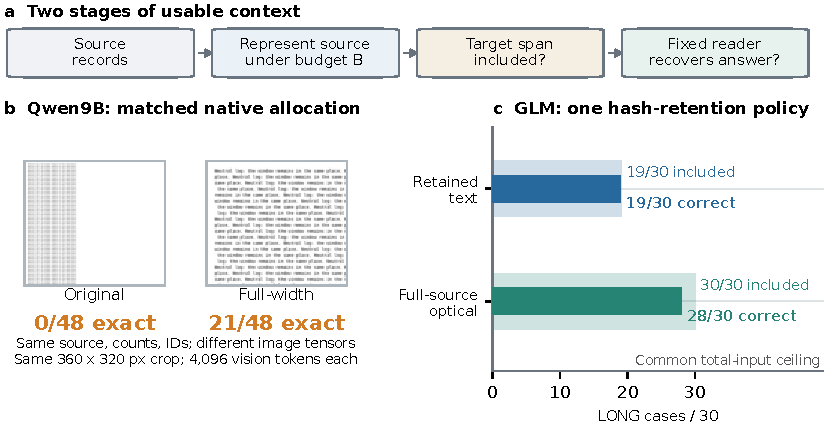
\includegraphics[width=\linewidth]{figures/figure1.pdf}
\caption{\textbf{Matched allocation does not establish target inclusion or recovery.} (a) Inclusion and conditional recovery are separate measurements; a correct guess need not imply inclusion. (b) Qwen9B's Original and Full-width layouts preserve the source, native counts, and input IDs (4,096 vision tokens), yet recover 0/48 versus \nval{layout.Qwen9B.efficient_c2_p4}/48 identifiers. Identical top-left $360\times320$-pixel crops illustrate occupied geometry; full pages determine the outcomes. (c) Under the hash-retention policy, GLM's LONG text includes and answers 19/30 targets; full-source optical input includes 30/30 and answers \nval{budget.GLM.long.optical}/30 at the same total-input upper bound. Only GLM establishes a corrected LONG advantage. Fresh compact-text control: Section~\ref{sec:budget}. Panels (b) and (c) use different cases and readers.}
\label{fig:overview}
\end{figure}

\section{Native budgets, target inclusion, and conditional recovery}
Let $X$ be the source, $\tilde X$ the source content assigned to the representation, $V$ the measured vision-token count, and $N_M$ reader $M$'s source-text token count. Optical rate and token-level source coverage are
\begin{equation}
r=\frac{V}{N_M(\tilde X)},\qquad \rho=\frac{N_M(\tilde X)}{N_M(X)}.
\label{eq:accounting}
\end{equation}
We report rate's reciprocal, $C_{\mathrm{eff}}=1/r$, as realized visual density so it can be compared with the nominal renderer targets $C\in\{0.8,2,4\}$. It counts included-source tokens per vision token, not original-source tokens per total input token. Full-source optical input has $\tilde X=X$; with selection, $V/N_M(X)=r\rho$. Retained text has no optical rate and is compared under the native \emph{total-input} ceiling $B$, which includes prompt overhead and is not a physical storage-byte budget. Vision tokens are processor-specific units, not bits; rate--distortion theory supplies only the distinction between rate and loss, not an optimality claim \citep[Chapter~10]{coverthomas}.

For single-target binary correctness $Y$, let $\tau$ indicate inclusion of the requested record. Conditional recovery is $P(Y=1\mid\tau=1)$; overall success obeys the accounting identity
\begin{equation}
\begin{split}
P(Y=1)={}&P(\tau=1)P(Y=1\mid\tau=1)\\
         &+P(\tau=0)P(Y=1\mid\tau=0).
\end{split}
\label{eq:success}
\end{equation}
Token coverage $\rho$ does not determine target inclusion $\tau$. Inclusion means that the audited source span was assigned to the reader's representation, not that perceptually distinct characters survived its visual encoding. Correct answers to omitted targets are possible through guessing or prior knowledge; none occurs in our retained-text synthetic cases. For task loss $D_{\mathrm{task}}=\mathbb{E}[L(A,\hat A)]$, $L$ is one minus the study's EM, native retrieval score, or normalized F1, with its stated sampling weights. Lower loss means better overall task performance, not necessarily better conditional recovery. LoCoMo may require multiple evidence spans; we do not estimate its evidence-inclusion decomposition.

Pre-query retention $S_{\mathrm{store}}(X;B)$ commits content before the question and cannot retrieve discarded records; query-time selection $S_{\mathrm{query}}(X,Q;B)$ can consult the full source using the question. The original hash study conditions fit on actual question overhead; the compact-text follow-up uses a fixed future-query reserve and commits both text representations strictly before the query. LoCoMo BM25 instead studies query-time selection. Preparation, prefill, latency, and memory remain separate costs: neither native token rate nor equal total input counts determine them.

\section{Experimental setting}
We evaluate Qwen3.5-2B (Qwen2B), Qwen3.5-9B (Qwen9B), and GLM-4.6V-Flash (GLM), with pinned model and processor snapshots \citep{qwen,glm}. Readers are not fine-tuned for our experiments. Greedy decoding, native prompts, and generation caps are frozen within each study. The original study contains 500 LoCoMo-derived questions from ten conversations, 180 RULER-derived cases across six task configurations, and 96 controlled identifier cases. The geometry follow-ups use distinct held-out sets of 48 and 32 cases; fixed-budget retrieval uses 30 paired base cases at three lengths. A separate GLM compact-text follow-up uses 150 fresh LONG sources and three paired representations. We keep these samples separate rather than pooling interventions across studies.

Metrics reflect the requested information. LoCoMo uses normalized answer F1, averaged equally across conversations. RULER uses its scoped task-native containment scores, including partial credit for multiple targets; these scores are not exact-output accuracy. Identifiers use canonical exact match (EM), which normalizes the frozen answer representation without accepting arbitrary explanatory prose. Both finite-budget studies use native single-answer containment, with EM and character error rate (CER) as diagnostics. An identifier prompt includes a worked example. The synthetic experiments are diagnostic tasks, not evaluations of an interactive agent.

Uncertainty follows the sampling unit: conversations for LoCoMo and paired cases for the controlled studies. We preserve each study's prospective testing family. Reported bootstrap intervals are pointwise 95\% intervals, not simultaneous intervals. The appendix gives full tests, sample construction, decoder settings, and provenance. 

Generative AI language tools assisted with experimental implementation and audit code, synthetic diagnostics, literature discovery, manuscript drafting and editing, and feedback on the compact-text protocol and interpretation. The authors checked the code, analyses, claims, and references against preserved evidence. 

\section{Geometry changes recovery at matched measured rate}
\label{sec:geometry}
A visual-token count alone cannot specify exact recovery if different image geometries at the same native allocation yield different results. Exact identifiers offer a demanding test because plausible paraphrases cannot replace the requested string.

The original identifier study recovers \nval{id.Qwen2B.full_raw}/96, \nval{id.Qwen9B.full_raw}/96, and \nval{id.GLM.full_raw}/96 values from text, but none of the 1,152 answers across compressed $C=2$ and $C=4$ arms is exact. Source-span auditing confirms that the represented text is present. Geometric inspection instead reveals an unusually narrow occupied region and small effective glyphs. This motivates intervention on representation geometry rather than an information-capacity interpretation of the failures.

\paragraph{Matched-budget layout intervention.}
We select an answer-blind full-width wrapping layout using a separate development set and evaluate 48 fresh held-out cases. Original and full-width conditions preserve the source string, native vision/nonvision/total counts, input-ID sequences, and recorded image-grid allocation. The IDs fix text and image-placeholder positions; image tensors and their visual embeddings differ. This is matched allocation, not identical effective neural input. Both retain the complete source across four pages. The layout package changes wrapping, whitespace, and pagination jointly.

\begin{figure}[t]
\centering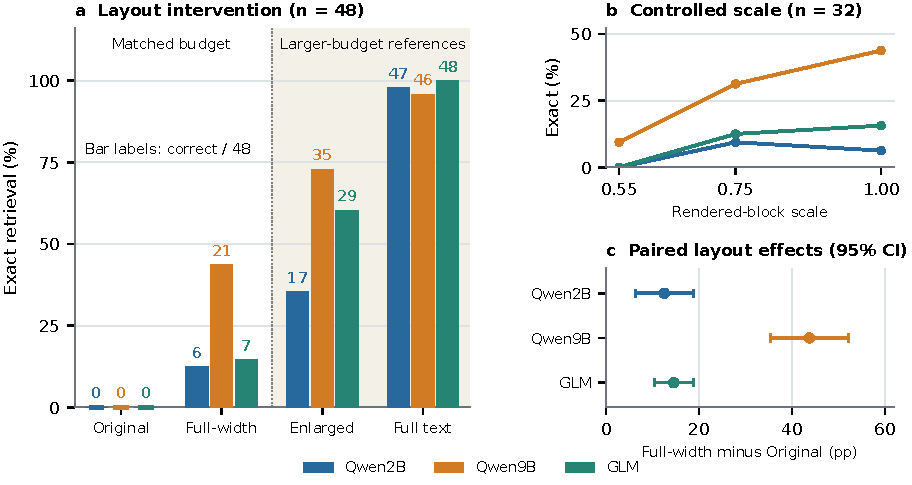
\includegraphics[width=\linewidth]{figures/geometry.pdf}
\caption{\textbf{Geometry changes recovery at matched native allocation.} (a) Original and Full-width are the matched-budget comparison. Shaded Enlarged and Full text are larger-budget diagnostic references; neither is a matched-budget alternative. Labels give exact successes out of 48. (b) Independent scale triplets hold source, wrapping, pagination, canvas, and counts fixed; only Qwen9B passes the corrected primary test. (c) Paired Full-width minus Original effects with pointwise 95\% design-stratified bootstrap intervals; each cell contains only two cases. The layout and scale studies use different cases (Appendix~\ref{app:geometry}).}
\label{fig:geometry}
\end{figure}

Exact retrieval rises from zero in the original layout to \nval{layout.Qwen2B.efficient_c2_p4}/48, \nval{layout.Qwen9B.efficient_c2_p4}/48, and \nval{layout.GLM.efficient_c2_p4}/48 (Figure~\ref{fig:geometry}a). All three paired exact McNemar tests pass Holm correction. This establishes different exact-recovery rates for different layouts at the same measured native allocation, not a new information-theoretic bound. Absolute optical recovery remains below the full-text controls: even enlarged-image controls reach only \nval{layout.Qwen2B.readable_p4}/48, \nval{layout.Qwen9B.readable_p4}/48, and \nval{layout.GLM.readable_p4}/48, all below the prespecified 36/48 criterion. Figure~\ref{fig:geometry} shows the remaining deficit to full text and the paired uncertainty; the enlarged and full-text references spend more input tokens than the matched layouts.

\paragraph{Controlled rendered-block scale.}
To narrow the intervention, we render each of 32 fresh cases once, then uniformly scale the page content to 0.55, 0.75, or 1.00 and center it on the same final canvas. Line breaks, page assignments, source, question, and native input counts remain fixed. This removes reflow and pagination changes while varying occupied area and effective visual scale.

Qwen9B exact recovery increases from \nval{scale.Qwen9B.0.55.correct}/32 to \nval{scale.Qwen9B.0.75.correct}/32 to \nval{scale.Qwen9B.1.00.correct}/32. The exact conditional Cochran $Q$ test is significant after correction across readers ($p=\nval{scale.Qwen9B.holm}$). Its endpoint difference is \nval{scale.Qwen9B.0.effect} percentage points (95\% interval [\nval{scale.Qwen9B.0.lo}, \nval{scale.Qwen9B.0.hi}]); the endpoint test also passes the separate nine-comparison family. Qwen2B yields \nval{scale.Qwen2B.0.55.correct}, \nval{scale.Qwen2B.0.75.correct}, and \nval{scale.Qwen2B.1.00.correct} successes; GLM yields \nval{scale.GLM.0.55.correct}, \nval{scale.GLM.0.75.correct}, and \nval{scale.GLM.1.00.correct}. Neither passes its corrected primary test. All ten generation-cap hits remain in the analysis.

Together, the interventions establish a matched-allocation layout effect across readers and a narrower scale response for Qwen9B. Uniform scaling still changes glyph size, occupied area, resampling, and physical positions together. It neither isolates glyph height alone nor establishes a universal monotonic law. Qwen2B's observed response is nonmonotonic; a difference in significance across readers does not establish a reader-by-scale interaction.

\section{Source coverage under a fixed input budget}
\label{sec:budget}
When full text no longer fits, pre-query storage may omit a future target. We construct 30 fresh single-key cases with SHORT, MEDIUM, and LONG versions that preserve the query and target while adding distractors. Optical input renders the complete source on four pages. Text greedily retains complete hash-ranked records while the native templated input fits the same reader-specific ceiling, then restores source order. Ranking is query-independent, but fit reserves actual question overhead; strictly pre-query storage instead needs a fixed reserve. Omitted records are unavailable. This $S_{\mathrm{store}}$ diagnostic bounds native input, not storage bytes or an optimized memory policy. Query-time lookup with access to discarded records is untested; LoCoMo BM25 separately studies selection from the complete history.

Full text fits at SHORT. Source length is approximately one-half, one-and-a-half, and twice the nominal text-source capacity across the three regimes (Figure~\ref{fig:budget}). The constraint is an equal total-input upper bound, not equal consumed tokens: SHORT text is not padded. Optical renders the complete source in all regimes, with target spans audited as included; its realized visual density therefore increases with length. Appendix~\ref{app:budget} gives native budgets and target-retention diagnostics.

\begin{figure}[t]
\centering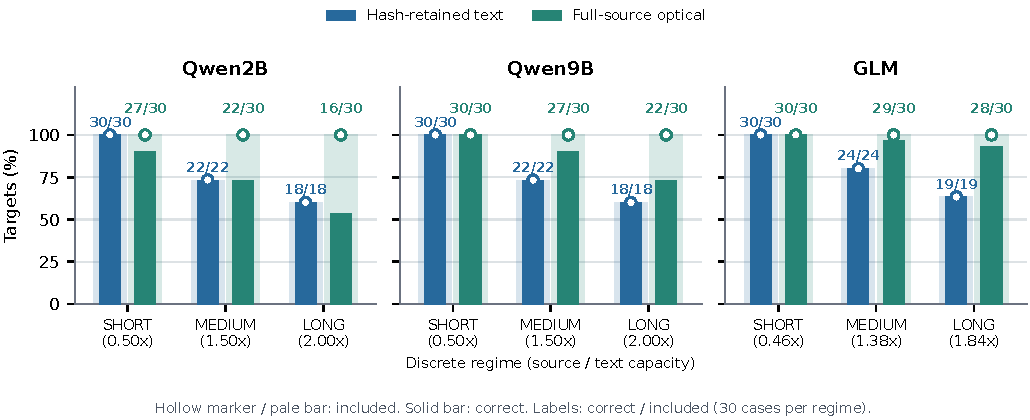
\includegraphics[width=\linewidth]{figures/budget.pdf}
\caption{\textbf{Inclusion and correctness under one hash-retention policy.} Each regime has 30 paired cases and a common total-input upper bound, not equal consumed tokens. Pale bars and hollow markers show included targets; solid bars show correct answers. Labels are correct/included counts: text recovers every retained target, while optical includes all 30 but can fail to recover them. Only GLM establishes a corrected LONG advantage. Source/capacity ratios are nominal; complete templated-input checks govern fit (Appendix~\ref{app:budget}).}
\label{fig:budget}
\end{figure}


Under this hash-retention policy, GLM recovers \nval{budget.GLM.long.optical}/30 LONG targets from optical input versus \nval{budget.GLM.long.text}/30 from retained text, a \nval{budget.GLM.secondary_long.effect}-point difference (95\% interval [\nval{budget.GLM.secondary_long.lo}, \nval{budget.GLM.secondary_long.hi}]; adjusted $p=\nval{budget.GLM.secondary_long.holm}$). Precisely \nval{budget.GLM.long.text}/30 queried records survive in the GLM text input, and every one is answered correctly; the optical input includes all 30 target spans but has two recovery failures. The primary interaction passes its separate corrected family with the same value. Because GLM ties at SHORT on every case, the LONG and interaction tests are the same case-level contrast, not independent confirmations. Qwen9B's LONG difference is positive but uncertain; Qwen2B's is negative (Figure~\ref{fig:budget}; all interaction tests appear in Appendix~\ref{app:budget}, Table~\ref{tab:budget}).

At every length and for every reader, text answers every surviving target and no omitted target. Optical includes the full source but sometimes fails on an included target. For GLM LONG, greater inclusion outweighs imperfect recovery: conditional text recovery is \nval{budget.GLM.long.text}/\nval{budget.GLM.long.text}, versus optical \nval{budget.GLM.long.optical}/30, with \nval{derived.budget.GLM.long.gains} optical-only and \nval{derived.budget.GLM.long.losses} text-only successes. The balance is less favorable for the Qwen readers. Token coverage alone would not establish these case-level facts.

No reader meets the prespecified descriptive crossover rule, which requires text to be strictly better at SHORT and optical strictly better at LONG. GLM and Qwen9B tie at SHORT; Qwen2B does not win optically at LONG. The original primary sign-flip test assumes conditional sign symmetry of case interactions; its uncertainty is conditional on these 30 cases and their construction.

\paragraph{Compact pre-query text control.}
On \nval{compact.n} fresh sources, we prospectively test GLM's positive LONG operating point. Both text arms use the same pre-query hash priority and fixed query reserve; compact key/value lines retain \nval{compact.capacity_gain}\% more records. At a common \nval{compact.B}-token ceiling, optical answers \nval{compact.optical.successes}/\nval{compact.n}, compact text \nval{compact.compact_text.successes}/\nval{compact.n}, and original-format text \nval{compact.hash_text.successes}/\nval{compact.n}. The primary optical--compact difference is \nval{compact.effect} points (95\% stratified paired bootstrap interval [\nval{compact.lo}, \nval{compact.hi}]; exact McNemar $p=\nval{compact.p}\times10^{-6}$). Text recovers every included target; optical includes all but misses \nval{compact.optical.misses}. The ceiling was amended before inference, \nval{compact.budget_increase}\% above the original budget (Appendix~\ref{app:compact}, including conservative sensitivity and position diagnostics). This supports the specific compact control, not optimized memory or query-time retrieval with source access.

\section{Density-dependent retrieval within one rendering family}
\label{sec:density}
How does retrieval change as the same source is rendered more densely within one page-construction procedure? We use six RULER-derived configurations, with 30 cases each at an upstream reference length of 8,192 tokens \citep{ruler}. Each case is evaluated as text and on four optical pages at nominal $C\in\{0.8,2,4\}$. Native processors determine the realized token counts; a shared nominal ratio does not imply identical pixels across readers. The same renderer produced the original identifier pages in Section~\ref{sec:geometry}, but the realized geometries differ: audited median maximum horizontal text span across four-page inputs is 77.9\% of page width here versus 12.3\% for the original identifiers (Appendix~\ref{app:original}). The identifier study's narrow-column failure therefore should not be projected onto this sweep.

\begin{figure}[t]
\centering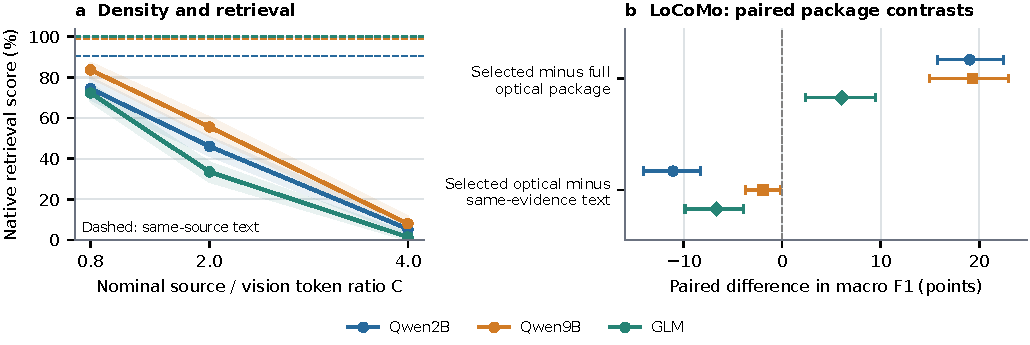
\includegraphics[width=\linewidth]{figures/frontiers.pdf}
\caption{\textbf{Density and selection change task performance in different ways.} (a) Six-task RULER aggregate across nominal renderer targets; Table~\ref{tab:rates} reports realized density. Shading gives pointwise task-stratified 95\% intervals; dashed lines show same-source text. (b) Paired LoCoMo contrasts: selected minus full optical measures a selection-plus-rendering package; selected optical minus same-evidence text compares modalities. Intervals resample ten conversations and are pointwise. Condition means appear in Table~\ref{tab:locomo}; no continuous frontier or isolated retrieval effect is implied.}
\label{fig:frontiers}
\end{figure}

Figure~\ref{fig:frontiers}a shows a steep decline for every reader. At $C=0.8$, task-native scores are \nval{ruler.Qwen2B.optical_c0p8_p4}, \nval{ruler.Qwen9B.optical_c0p8_p4}, and \nval{ruler.GLM.optical_c0p8_p4}\%; at $C=4$, they are \nval{ruler.Qwen2B.optical_c4_p4}, \nval{ruler.Qwen9B.optical_c4_p4}, and \nval{ruler.GLM.optical_c4_p4}\%. Same-source text reaches \nval{ruler.Qwen2B.full_raw}, \nval{ruler.Qwen9B.full_raw}, and \nval{ruler.GLM.full_raw}\%. Thus even the least dense optical setting has a lower six-task aggregate in this rendering family. Individual tasks differ: Qwen2B variable tracking scores \nval{rulertask.Qwen2B.optical_c0p8_p4.vt}\% optically at $C=0.8$ versus \nval{rulertask.Qwen2B.full_raw.vt}\% as text (Appendix~\ref{app:original}). These are selected-task operating points, not a universal capacity threshold or the official RULER aggregate.

\begin{table}[t]
\centering\small
\caption{\textbf{Realized RULER visual density.} Median per-case $C_{\mathrm{eff}}=N_M(X)/V$ at each nominal target. Both Qwen readers have the same recorded counts. Appendix~\ref{app:original} gives native counts and ranges.}
\label{tab:rates}\begin{tabular}{lrrr}
\toprule
Reader & Nominal $C=0.8$ & $C=2$ & $C=4$\\
\midrule
Qwen2B / Qwen9B & \nval{derived.rates.Qwen2B.optical_c0p8_p4.Cmed} & \nval{derived.rates.Qwen2B.optical_c2_p4.Cmed} & \nval{derived.rates.Qwen2B.optical_c4_p4.Cmed}\\
GLM & \nval{derived.rates.GLM.optical_c0p8_p4.Cmed} & \nval{derived.rates.GLM.optical_c2_p4.Cmed} & \nval{derived.rates.GLM.optical_c4_p4.Cmed}\\
\bottomrule\end{tabular}

\end{table}

These results do not directly contradict \emph{Text or Pixels?} \citep{textpixels}: its single-needle experiments use different readers, shorter contexts, and a different renderer, and also show degradation beyond successful operating ranges. Our task mixture and protocol do not reproduce that setting; they cannot identify which difference explains a cross-paper gap.

Scoring matters to this conclusion. A frozen diagnostic sample of 20 Qwen text answers that passed native retrieval but failed canonical EM all contained the target with extra prose or Markdown. Such disagreements cannot be read as retrieval failures. We retain native scores as primary and report stricter formatting diagnostics separately. This distinction becomes consequential for identifiers, where every character of the returned value is part of the task.

\section{Evidence selection and rendering shift the operating point}
\label{sec:selection}
How does a query-time selected optical package perform when it represents less irrelevant conversation history? On LoCoMo \citep{locomo}, we compare complete histories with the top 16 turns selected by a frozen BM25 retriever conditioned on the question but never on its answer. This is query-time selection, $S_{\mathrm{query}}$, with the complete history available to the retriever. Retrieved text and retrieved optical consume the same canonical evidence string. Full optical uses approximately $C=2$; retrieved optical uses a fixed single-page rendering. Two additional textual controls pack whole turns to the respective optical input budgets.

\begin{table}[t]
\centering
\caption{\textbf{LoCoMo conversation-macro F1.} All conditions answer the same 500 questions. Retrieved text and optical share evidence; the two budgeted-text controls may retain different turns.}
\label{tab:locomo}
\begin{tabular}{lrrr}
\toprule
Representation & Qwen2B & Qwen9B & GLM\\
\midrule
Full text & \nval{loc.Qwen2B.full_raw.conversation_macro_f1} & \nval{loc.Qwen9B.full_raw.conversation_macro_f1} & \nval{loc.GLM.full_raw.conversation_macro_f1}\\
Full optical & \nval{loc.Qwen2B.full_optical_c2.conversation_macro_f1} & \nval{loc.Qwen9B.full_optical_c2.conversation_macro_f1} & \nval{loc.GLM.full_optical_c2.conversation_macro_f1}\\
Retrieved text & \nval{loc.Qwen2B.retrieved_text.conversation_macro_f1} & \nval{loc.Qwen9B.retrieved_text.conversation_macro_f1} & \nval{loc.GLM.retrieved_text.conversation_macro_f1}\\
Retrieved optical & \nval{loc.Qwen2B.retrieved_optical_8px.conversation_macro_f1} & \nval{loc.Qwen9B.retrieved_optical_8px.conversation_macro_f1} & \nval{loc.GLM.retrieved_optical_8px.conversation_macro_f1}\\
Text, full-optical budget & \nval{loc.Qwen2B.retrieved_text_matched.conversation_macro_f1} & \nval{loc.Qwen9B.retrieved_text_matched.conversation_macro_f1} & \nval{loc.GLM.retrieved_text_matched.conversation_macro_f1}\\
Text, selected-optical budget & \nval{loc.Qwen2B.retrieved_text_matched_selected.conversation_macro_f1} & \nval{loc.Qwen9B.retrieved_text_matched_selected.conversation_macro_f1} & \nval{loc.GLM.retrieved_text_matched_selected.conversation_macro_f1}\\
\bottomrule\end{tabular}

\end{table}

The selected optical package improves F1 over full optical by \nval{loc.Qwen2B.H1.effect}, \nval{loc.Qwen9B.H1.effect}, and \nval{loc.GLM.H1.effect} points (reader order Qwen2B, Qwen9B, GLM). Each contrast passes the frozen Holm family. The increase is large enough to move retrieved optical well away from the low full-optical scores, but it is an effect of the \emph{retrieved optical package}: selection changes evidence, context burden, layout, and rendering regime together. The experiment does not isolate retrieval as the sole causal mechanism.

With the evidence held equal, optical minus text is \nval{loc.Qwen2B.H2.effect}, \nval{loc.Qwen9B.H2.effect}, and \nval{loc.GLM.H2.effect} points. None establishes equivalence within the prespecified $\pm3$-point margin. Qwen9B's smaller gap is sensitive to the interval construction: its conversation-level $t$ interval crosses zero (Appendix~\ref{app:locomo}). The point estimates support a fidelity cost, with unequal precision across readers. Both budgeted-text controls also score above their optical counterparts for every reader (Table~\ref{tab:locomo}); changing the selected optical package does not establish a practical advantage over those text controls.

Generation length does not account for the large selection gains in the bounded sensitivity we tested. Rerunning only the 126 Qwen2B and 121 Qwen9B full-optical cap hits from 96 to 256 tokens changes reconstructed full-arm F1 by just \nval{cap.Qwen2B.macro_change} and \nval{cap.Qwen9B.macro_change} points. All reruns preserve their original generated-token prefixes. Some remain capped, so this diagnostic does not establish that generation length is irrelevant; it leaves the original primary results intact.

\section{Systems costs in two operating regimes}
\label{sec:systems}
We profile one predetermined source per length on an A100 40GB with resident BF16 models, SDPA, batch size one, and one generated token. Each of 45 cells has three warmups and ten measured repetitions; these measure execution variation, not accuracy or workload uncertainty. Appendix~\ref{app:systems} reports all timing boundaries and values, including allocated peaks both with and without the resident-model baseline.

For the same LONG source, C2 lowers combined prefill (including vision encoding) and allocated peak for every reader, but lowers end-to-end time only for Qwen9B. C4 lowers LONG end-to-end time for all three, without corresponding C4 quality evaluation on these inputs. In the fixed-budget comparison, optical has lower MEDIUM/LONG end-to-end time but higher prefill and allocated peak than retained text. Text packing repeatedly tokenizes subsets inside timing; optical layout planning and calibration are precomputed and excluded. Caching the text packer could change the ranking. These results distinguish preparation, model execution, and memory costs in the measured implementation; they establish neither quality-preserving nor intrinsic optical acceleration.

\section{Related work}
\label{sec:related}
\paragraph{Closest empirical comparisons.}
\emph{Text or Pixels?} evaluates fixed readers on rendered-text RULER retrieval and summarization, including rendering, token savings, and timing \citep{textpixels}. Fico studies fidelity across OCR, retrieval, and QA; binarization, JPEG, and upscale perturbations can change utility without changing the reported compression ratio \citep{fico}. AGAR studies evidence localization and recovery through span magnification, with a uniform-scaling control designed to match visual-token use; its reported aggregate counts are close, not identical \citep{agar}. These works already establish density and geometry sensitivity. We add an answer-blind, held-out exact-string layout intervention with identical per-case native vision, nonvision, and total counts and input IDs, followed by fixed-canvas scaling. These measure task-specific layout and scale effects without isolating a mechanism.

LensVLM distinguishes coverage from fidelity, analyzes conditional evidence hits, and tests selective expansion with trained and untrained readers \citep{lensvlm}. Neither that distinction nor fixed readers alone is new here. We audit target inclusion and answer success under frozen hash ranking, including a compact-text follow-up with a fixed pre-query reserve and no adaptive expansion. \citet{badauto} find optical language modeling comparable to truncation; factual recall, measured by answer log-likelihood, can improve over truncation but favors direct alternatives. Our GLM result concerns generated answers on one synthetic LONG task under specified original-format and compact hash-retention policies, not superiority to learned or query-aware alternatives.

Measure-transport analyses distinguish token savings from task-relevant visual loss; their coverage cost concerns cross-patch fragmentation rather than omitted source records \citep{measuretransport}. ZeroSense probes full-text recovery using low-predictability contexts to reduce semantic compensation \citep{zerosense}. Our measurements instead audit source-span inclusion and reader-specific answer recovery.

\begin{table}[t]
\centering\footnotesize
\caption{\textbf{Closest prior work and the comparison tested here.} This is a protocol map, not a cross-paper score ranking. The final column states this study's distinct \emph{measurement}, without claiming that earlier work lacked all related controls.}
\label{tab:positioning}
\begingroup\setlength{\tabcolsep}{3pt}
\begin{tabular}{@{}>{\raggedright\arraybackslash}p{.80in}>{\raggedright\arraybackslash}p{2.11in}>{\raggedright\arraybackslash}p{2.05in}@{}}\toprule
Work & Established result or design & Specific measurement here\\\midrule
Text or Pixels? & Fixed-reader rendered text; density limits, rendering and timing & Held-out exact-string geometry at matched native allocation\\
Fico & Fidelity perturbations, including unchanged-ratio conditions, across OCR, retrieval and QA & Paired reflow and fixed-canvas scale with audited native counts and IDs\\
LensVLM & Coverage/fidelity and conditional hit analysis; expansion with trained and untrained readers & Target inclusion and success under original and compact hash retention; actual-query or fixed-reserve packing\\
Lee et al. & Factual-recall benefit over truncation; direct alternatives outperform optical & Generated answers from fixed readers versus a specified hash policy\\
Glyph & Trained rendering search; similar-ratio configuration ablation; rare-string difficulty & Exact-string layout interventions preserving native allocation with unmodified readers\\
AGAR & Evidence magnification; fixed readers; approximately token-matched uniform scaling & Answer-blind static exact-string intervention with identical per-case native counts and IDs\\\bottomrule
\end{tabular}\endgroup

\end{table}

\paragraph{Systems and learned memory.}
DeepSeek-OCR trains an optical encoder--decoder and measures reconstruction across compression levels \citep{deepseekocr}. Glyph combines training with rendering search, ablates similar-ratio configurations, and identifies rare order-sensitive strings as difficult \citep{glyph}; our contribution is stricter native-allocation control, not discovering that fragility. VIST learns a resampler and cross-attention interface for distant visual context \citep{vist}. AgentOCR learns optical history compression through agentic reinforcement learning \citep{agentocr}; MemOCR learns layouts under budget-aware rewards \citep{memocr}. OCR-Memory fetches original text through optical anchors \citep{ocrmemory}; our comparator cannot access discarded records. VizoMem trains a visual-note retriever for conversational memory \citep{vizomem}. These systems use training, adaptive selection, or retrieval beyond our static representations.

Cross-paper score rankings would conflate readers, training, native accounting, rendering, tasks, and selection timing. Our internal controls compare the same source or evidence across modalities, match native allocation across layouts, and diagnose omission under original-format and compact hash-retention policies. The last comparison does not establish the best attainable textual memory. Table~\ref{tab:positioning} summarizes these boundaries.

\section{Discussion and limitations}
The experiments separate three quantities: measured representation rate, whether the requested source record or span is included in the reader input, and whether a fixed reader recovers an included target. The six-task RULER aggregate and LoCoMo condition means favor available text over the corresponding optical arms, with task-level exceptions in RULER. Under a finite input budget, hash-retained text can instead fail because it omits the requested record. GLM's LONG results, including the compact-text follow-up, show one regime where full-source optical inclusion outweighs imperfect recovery. They do not establish the same balance for another reader, untested retention policy, or memory workload.

Geometry and selection alter these stages through different routes. Matched layout changes recovery while leaving the represented source and native token allocation fixed. LoCoMo selection changes the evidence, context burden, and rendering package together, so its gains cannot be assigned to retrieval alone. Reporting a visual-token ratio without target inclusion and task recovery misses both a coverage benefit and a fidelity cost. Systems measurements add a separate distinction: lower end-to-end time need not mean lower prefill or peak allocation.

The scope is limited to three readers and selected benchmark subsets. Ten dialogue clusters and the small independent case sets constrain precision. Public benchmark exposure during training is unknown. Exact identifiers probe brittle state recovery rather than all memory use, and native containment does not establish verbatim reconstruction. Generation caps remain binding for some conditions. The unusually narrow original layout limits generalization to typical documents. The fresh geometry studies are separate samples; covarying visual dimensions prevent a glyph-only mechanism claim. Nonsignificance in other readers is not equivalence.

The finite-budget results depend on deterministic hash retention; the follow-up tests only one simple compact serializer on the previously positive GLM LONG operating point. Optimized textual memory and query-time retrieval with source access remain untested. Budgets count native input, not storage bytes. The original packer uses actual question overhead; the follow-up commits storage with a fixed reserve at a \nval{compact.budget_increase}\% larger ceiling. Similarly, local freezes establish prospective specification within this project, not independent preregistration. Systems results use one predetermined source per length, a single hardware setup, one-token output, and implementation-dependent preprocessing; they cannot establish workload-wide latency or compute savings. The appendix reports these boundaries alongside the complete secondary results.

\paragraph{Evaluation implications.}
A budgeted context evaluation can diagnose the two failure stages directly: record whether each requested source span reaches the reader, then report answer accuracy for included and omitted targets as well as overall accuracy. State whether selection occurs before the query or can still consult the complete source. For optical inputs, report processor-native vision, nonvision, and total counts together with representative rendered pages; for a geometry claim, pair cases and check input IDs. Measure representation preparation, prefill, and peak allocation separately when making systems claims. These checks make the tested operating point interpretable without assuming that token count predicts utility.

\section{Conclusion}
A visual-token count does not specify whether a future target is present or recoverable. At identical native allocation, geometry changes exact recovery. GLM answers more LONG targets optically than under original-format hash retention and a fresh compact-text control; the latter tests GLM only. Density, query-time selection, and systems profiles delimit these operating points. Compressed-context evaluations should report inclusion, conditional recovery, overall performance, native input counts, and execution costs separately.

\label{maintextend}
\bibliography{references}
\bibliographystyle{iclr2027_conference}
\clearpage
\appendix
\section{Protocols, samples, and statistical interpretation}
\label{app:methods}
The original experiments, the layout intervention, the bounded cap diagnostic, and the final studies retain their separate frozen designs. Local timestamped freezes precede each follow-up's evaluation outputs; they are not independently registered preregistrations. Development, smoke, historical legacy, and systems-timing outputs do not enter held-out task estimates.

\begin{table}[ht]
\centering\small
\caption{Evaluation inventory. Outputs are executions of conditions, not independent samples. The cap diagnostic is conditional on the original capped subset.}
\begin{tabular}{lrrl}\toprule
Study & Cases & Outputs & Independent unit\\\midrule
LoCoMo & 500 questions & 9,000 & 10 conversations\\
RULER-derived & 180 & 2,160 & Case, stratified by task\\
Original identifiers & 96 & 2,016 & Case, balanced factor design\\
Layout intervention & 48 & 576 & Paired held-out case\\
Controlled scale & 32 & 288 & Paired triplet\\
Fixed-budget retrieval & 30 base cases & 540 & Base case across lengths\\
Compact static storage & \nval{compact.n} & \nval{compact.calls} & Paired source triplet\\
LoCoMo cap sensitivity & 247 capped questions & 247 & Original conversation\\
Systems profiling & 1 source per length & 585 & Repeated invocation\\\bottomrule
\end{tabular}
\end{table}

The original study contributes 13,176 outputs. The layout intervention additionally uses 36 development calls on 12 cases, excluded from held-out estimates. The final round contributes 828 quality outputs and 585 profiling invocations, of which 135 are warmups and 450 are measured. The profiling instrumentation observes 585 top-level model forwards. This count does not measure internal forward calls of the quality runs or count their outputs as additional accuracy samples. The later compact-storage follow-up contributes \nval{compact.calls} additional quality outputs on \nval{compact.n} independent sources; its three answer-blind development sources and separate smoke cases do not enter estimates.

\paragraph{Decoding and scoring.}
The original LoCoMo, RULER-derived, and identifier caps are 96, 128, and 64 generated tokens, respectively. Both earlier final quality studies and the compact-storage follow-up use 64. Generation is greedy, with thinking disabled where the native interface supports that setting. The final studies use BF16, SDPA, batch one, and the inherited model generation configuration; the complete configuration accompanies each output. Token IDs are preserved as well as decoded text. Canonical identifier EM uses the frozen scorer's whitespace and answer normalization; it does not strip arbitrary prose to rescue an otherwise incorrect output. CER can exceed one when extra predicted characters outnumber reference characters. Literal-raw EM is a separate diagnostic because model-specific output wrappers can differ from the canonical answer.

\paragraph{Families and intervals.}
The original confirmatory family consists of three directional LoCoMo package tests and three original identifier contrasts. Its six-test Holm correction is retained. For LoCoMo H1, the statistic is the mean of ten paired conversation-level F1 differences, selected optical minus full optical. The one-sided upper-tail test enumerates all sign assignments, conditions on the observed magnitudes, and assumes sign symmetry under the null; condition assignment was not randomized. The LoCoMo same-evidence comparison estimates a difference and assesses a prespecified equivalence margin; it is not silently added as a new directional discovery. The RULER sweep is descriptive. Layout uses three two-sided exact McNemar tests in its own Holm family. Scale uses three exact conditional omnibus tests, with nine pairwise secondary tests in a separate family. Fixed-budget retrieval uses three primary interaction tests and a separate family of three secondary LONG tests. The compact-storage follow-up has one confirmatory optical--compact McNemar contrast, with other arm and position comparisons descriptive. There is no single global correction across these prospectively separated studies.

Paired percentile bootstrap intervals use 50,000 resamples. LoCoMo resamples whole conversations with equal weight, not individual questions. RULER resampling is stratified by task and keeps a case's representations together. Layout resampling is stratified within its 24 two-instance cells. With only two cases per cell, these intervals warrant caution: cells with identical observed differences contribute no bootstrap variation. The exact paired tests provide the confirmatory layout evidence. Scale and the original fixed-budget study resample paired cases; the compact-storage follow-up resamples paired triplets within its three position strata. These intervals are pointwise. Boundary intervals from zero successes or zero observed differences do not imply population certainty. Cluster sign tests and $t$ intervals below are sensitivity analyses, not additional confirmatory tests.

\section{Dialogue memory: complete comparisons and cap sensitivity}
\label{app:locomo}
The LoCoMo subset comprises the recorded 500 questions in ten previously studied conversation clusters, with 105, 108, and 287 questions in categories 1, 2, and 4. Expansion of question coverage does not create new independent conversations. We preserve dated chronological memories, speaker and turn identifiers, text, and shared-image captions. The BM25 retriever uses $k_1=1.5$, $b=0.75$, lowercase ASCII alphanumeric terms, and stable source-index tie-breaking. It selects the top 16 turns within the question's conversation and restores source order. It never uses reference answers, evidence annotations, or reader scores.

The same-evidence text and optical conditions receive identical canonical strings and turn metadata. Retrieved optical uses a single 1,372-pixel square RGB page, an 8-pixel source font, and 24-pixel margins. Full optical is calibrated to approximately $C=2$. The full-optical-budget text control greedily packs whole turns using the same ranking and skips oversized turns. The selected-optical-budget text control uses the frozen ranked-prefix rule without splitting turns or skipping an earlier ranked turn. These controls share a budget with their optical counterpart, not necessarily the same evidence.

\begin{table}[ht]\centering\small
\caption{All principal LoCoMo paired differences, in F1 points. H1: retrieved optical minus full optical. H2: retrieved optical minus same-evidence text. Selected/full budget: the relevant optical arm minus its budgeted-text control.}
\begin{tabular}{llrr}
\toprule
Reader & Contrast & Difference (F1 points) & 95\% interval\\
\midrule
Qwen2B & H1 & \nval{loc.Qwen2B.H1.effect} & [\nval{loc.Qwen2B.H1.lo}, \nval{loc.Qwen2B.H1.hi}]\\
Qwen2B & H2 & \nval{loc.Qwen2B.H2.effect} & [\nval{loc.Qwen2B.H2.lo}, \nval{loc.Qwen2B.H2.hi}]\\
Qwen2B & selected\_budget & \nval{loc.Qwen2B.selected_budget.effect} & [\nval{loc.Qwen2B.selected_budget.lo}, \nval{loc.Qwen2B.selected_budget.hi}]\\
Qwen2B & full\_budget & \nval{loc.Qwen2B.full_budget.effect} & [\nval{loc.Qwen2B.full_budget.lo}, \nval{loc.Qwen2B.full_budget.hi}]\\
Qwen9B & H1 & \nval{loc.Qwen9B.H1.effect} & [\nval{loc.Qwen9B.H1.lo}, \nval{loc.Qwen9B.H1.hi}]\\
Qwen9B & H2 & \nval{loc.Qwen9B.H2.effect} & [\nval{loc.Qwen9B.H2.lo}, \nval{loc.Qwen9B.H2.hi}]\\
Qwen9B & selected\_budget & \nval{loc.Qwen9B.selected_budget.effect} & [\nval{loc.Qwen9B.selected_budget.lo}, \nval{loc.Qwen9B.selected_budget.hi}]\\
Qwen9B & full\_budget & \nval{loc.Qwen9B.full_budget.effect} & [\nval{loc.Qwen9B.full_budget.lo}, \nval{loc.Qwen9B.full_budget.hi}]\\
GLM & H1 & \nval{loc.GLM.H1.effect} & [\nval{loc.GLM.H1.lo}, \nval{loc.GLM.H1.hi}]\\
GLM & H2 & \nval{loc.GLM.H2.effect} & [\nval{loc.GLM.H2.lo}, \nval{loc.GLM.H2.hi}]\\
GLM & selected\_budget & \nval{loc.GLM.selected_budget.effect} & [\nval{loc.GLM.selected_budget.lo}, \nval{loc.GLM.selected_budget.hi}]\\
GLM & full\_budget & \nval{loc.GLM.full_budget.effect} & [\nval{loc.GLM.full_budget.lo}, \nval{loc.GLM.full_budget.hi}]\\
\bottomrule\end{tabular}

\end{table}

H1 adjusted $p$ values are \nval{loc.Qwen2B.H1.holm}, \nval{loc.Qwen9B.H1.holm}, and \nval{loc.GLM.H1.holm}. The Qwen readers improve in all ten conversations; GLM improves in eight. GLM's directional sign test is less decisive than the original magnitude-sensitive sign-flip test. All leave-one-conversation-out H1 point estimates remain positive. For H2, the Qwen9B $t$ interval crosses zero even though its percentile bootstrap interval is below zero. Neither that sensitivity nor failure of the equivalence criterion licenses an equivalence claim.

\begin{table}[ht]\centering\small
\caption{Conversation-level sensitivity. $+/-$ count positive/negative differences. Sign $p_+$ tests a positive direction and should not be interpreted as a test of disadvantage for H2. Intervals are descriptive $t$ intervals over ten cluster differences.}
\begin{tabular}{llrrrrr}
\toprule
Reader & Contrast & $+$ & $-$ & Ties & Sign $p_+$ & $t$ interval (pp)\\
\midrule
Qwen2B & H1 & \nval{sens.0.positive} & \nval{sens.0.negative} & \nval{sens.0.ties} & \nval{sens.0.sign_p_greater} & [\nval{sens.0.lo}, \nval{sens.0.hi}]\\
Qwen2B & H2 & \nval{sens.1.positive} & \nval{sens.1.negative} & \nval{sens.1.ties} & \nval{sens.1.sign_p_greater} & [\nval{sens.1.lo}, \nval{sens.1.hi}]\\
Qwen9B & H1 & \nval{sens.2.positive} & \nval{sens.2.negative} & \nval{sens.2.ties} & \nval{sens.2.sign_p_greater} & [\nval{sens.2.lo}, \nval{sens.2.hi}]\\
Qwen9B & H2 & \nval{sens.3.positive} & \nval{sens.3.negative} & \nval{sens.3.ties} & \nval{sens.3.sign_p_greater} & [\nval{sens.3.lo}, \nval{sens.3.hi}]\\
GLM & H1 & \nval{sens.4.positive} & \nval{sens.4.negative} & \nval{sens.4.ties} & \nval{sens.4.sign_p_greater} & [\nval{sens.4.lo}, \nval{sens.4.hi}]\\
GLM & H2 & \nval{sens.5.positive} & \nval{sens.5.negative} & \nval{sens.5.ties} & \nval{sens.5.sign_p_greater} & [\nval{sens.5.lo}, \nval{sens.5.hi}]\\
\bottomrule\end{tabular}

\end{table}

\paragraph{Bounded cap follow-up.}
Precisely the original 126 Qwen2B and 121 Qwen9B full-optical cap hits are rerun once at 256 tokens. All original first-96-token prefixes match, permitting a cap-extension interpretation. Original uncapped answers remain in the reconstructed full arm. Qwen2B's macro F1 changes from \nval{cap.Qwen2B.full_500_conversation_macro_old} to \nval{cap.Qwen2B.full_500_conversation_macro_sensitivity}, a \nval{cap.Qwen2B.macro_change}-point change [\nval{cap.Qwen2B.lo}, \nval{cap.Qwen2B.hi}]. Qwen9B changes from \nval{cap.Qwen9B.full_500_conversation_macro_old} to \nval{cap.Qwen9B.full_500_conversation_macro_sensitivity}, a \nval{cap.Qwen9B.macro_change}-point change [\nval{cap.Qwen9B.lo}, \nval{cap.Qwen9B.hi}]. Neither reaches the prespecified three-point descriptive materiality threshold. There are still \nval{cap.Qwen2B.still_capped_256} and \nval{cap.Qwen9B.still_capped_256} cap hits, respectively. The diagnostic preserves the original primary tests and does not justify extrapolation to unlimited decoding.

\section{RULER-derived retrieval and original exact identifiers}
\label{app:original}
The RULER-derived subset uses \texttt{niah\_single\_1}, \texttt{niah\_single\_2}, \texttt{niah\_single\_3}, \texttt{niah\_multikey\_3}, \texttt{niah\_multivalue}, and \texttt{vt}. A pinned reference tokenizer generates one upstream sequence-length setting, 8,192 tokens. This setting does not promise precisely that many source tokens for every reader. The generator's insertion distributions, templates, and source backgrounds are preserved; native prompts are shared across modalities. Native multiple-answer metrics admit partial credit. The aggregate equally weights the six configurations.

\begin{table}[ht]\centering\small
\caption{Complete task-level RULER-derived native scores (percent). MK3: multikey 3; MV: multivalue; S1--S3: single 1--3; VT: variable tracking. The optical conditions all use four pages.}
\begin{tabular}{llrrrrrr}
\toprule
Reader & $C$ & MK3 & MV & S1 & S2 & S3 & VT\\
\midrule
Qwen2B & Text & \nval{rulertask.Qwen2B.full_raw.niah_multikey_3} & \nval{rulertask.Qwen2B.full_raw.niah_multivalue} & \nval{rulertask.Qwen2B.full_raw.niah_single_1} & \nval{rulertask.Qwen2B.full_raw.niah_single_2} & \nval{rulertask.Qwen2B.full_raw.niah_single_3} & \nval{rulertask.Qwen2B.full_raw.vt}\\
Qwen2B & 0.8 & \nval{rulertask.Qwen2B.optical_c0p8_p4.niah_multikey_3} & \nval{rulertask.Qwen2B.optical_c0p8_p4.niah_multivalue} & \nval{rulertask.Qwen2B.optical_c0p8_p4.niah_single_1} & \nval{rulertask.Qwen2B.optical_c0p8_p4.niah_single_2} & \nval{rulertask.Qwen2B.optical_c0p8_p4.niah_single_3} & \nval{rulertask.Qwen2B.optical_c0p8_p4.vt}\\
Qwen2B & 2 & \nval{rulertask.Qwen2B.optical_c2_p4.niah_multikey_3} & \nval{rulertask.Qwen2B.optical_c2_p4.niah_multivalue} & \nval{rulertask.Qwen2B.optical_c2_p4.niah_single_1} & \nval{rulertask.Qwen2B.optical_c2_p4.niah_single_2} & \nval{rulertask.Qwen2B.optical_c2_p4.niah_single_3} & \nval{rulertask.Qwen2B.optical_c2_p4.vt}\\
Qwen2B & 4 & \nval{rulertask.Qwen2B.optical_c4_p4.niah_multikey_3} & \nval{rulertask.Qwen2B.optical_c4_p4.niah_multivalue} & \nval{rulertask.Qwen2B.optical_c4_p4.niah_single_1} & \nval{rulertask.Qwen2B.optical_c4_p4.niah_single_2} & \nval{rulertask.Qwen2B.optical_c4_p4.niah_single_3} & \nval{rulertask.Qwen2B.optical_c4_p4.vt}\\
Qwen9B & Text & \nval{rulertask.Qwen9B.full_raw.niah_multikey_3} & \nval{rulertask.Qwen9B.full_raw.niah_multivalue} & \nval{rulertask.Qwen9B.full_raw.niah_single_1} & \nval{rulertask.Qwen9B.full_raw.niah_single_2} & \nval{rulertask.Qwen9B.full_raw.niah_single_3} & \nval{rulertask.Qwen9B.full_raw.vt}\\
Qwen9B & 0.8 & \nval{rulertask.Qwen9B.optical_c0p8_p4.niah_multikey_3} & \nval{rulertask.Qwen9B.optical_c0p8_p4.niah_multivalue} & \nval{rulertask.Qwen9B.optical_c0p8_p4.niah_single_1} & \nval{rulertask.Qwen9B.optical_c0p8_p4.niah_single_2} & \nval{rulertask.Qwen9B.optical_c0p8_p4.niah_single_3} & \nval{rulertask.Qwen9B.optical_c0p8_p4.vt}\\
Qwen9B & 2 & \nval{rulertask.Qwen9B.optical_c2_p4.niah_multikey_3} & \nval{rulertask.Qwen9B.optical_c2_p4.niah_multivalue} & \nval{rulertask.Qwen9B.optical_c2_p4.niah_single_1} & \nval{rulertask.Qwen9B.optical_c2_p4.niah_single_2} & \nval{rulertask.Qwen9B.optical_c2_p4.niah_single_3} & \nval{rulertask.Qwen9B.optical_c2_p4.vt}\\
Qwen9B & 4 & \nval{rulertask.Qwen9B.optical_c4_p4.niah_multikey_3} & \nval{rulertask.Qwen9B.optical_c4_p4.niah_multivalue} & \nval{rulertask.Qwen9B.optical_c4_p4.niah_single_1} & \nval{rulertask.Qwen9B.optical_c4_p4.niah_single_2} & \nval{rulertask.Qwen9B.optical_c4_p4.niah_single_3} & \nval{rulertask.Qwen9B.optical_c4_p4.vt}\\
GLM & Text & \nval{rulertask.GLM.full_raw.niah_multikey_3} & \nval{rulertask.GLM.full_raw.niah_multivalue} & \nval{rulertask.GLM.full_raw.niah_single_1} & \nval{rulertask.GLM.full_raw.niah_single_2} & \nval{rulertask.GLM.full_raw.niah_single_3} & \nval{rulertask.GLM.full_raw.vt}\\
GLM & 0.8 & \nval{rulertask.GLM.optical_c0p8_p4.niah_multikey_3} & \nval{rulertask.GLM.optical_c0p8_p4.niah_multivalue} & \nval{rulertask.GLM.optical_c0p8_p4.niah_single_1} & \nval{rulertask.GLM.optical_c0p8_p4.niah_single_2} & \nval{rulertask.GLM.optical_c0p8_p4.niah_single_3} & \nval{rulertask.GLM.optical_c0p8_p4.vt}\\
GLM & 2 & \nval{rulertask.GLM.optical_c2_p4.niah_multikey_3} & \nval{rulertask.GLM.optical_c2_p4.niah_multivalue} & \nval{rulertask.GLM.optical_c2_p4.niah_single_1} & \nval{rulertask.GLM.optical_c2_p4.niah_single_2} & \nval{rulertask.GLM.optical_c2_p4.niah_single_3} & \nval{rulertask.GLM.optical_c2_p4.vt}\\
GLM & 4 & \nval{rulertask.GLM.optical_c4_p4.niah_multikey_3} & \nval{rulertask.GLM.optical_c4_p4.niah_multivalue} & \nval{rulertask.GLM.optical_c4_p4.niah_single_1} & \nval{rulertask.GLM.optical_c4_p4.niah_single_2} & \nval{rulertask.GLM.optical_c4_p4.niah_single_3} & \nval{rulertask.GLM.optical_c4_p4.vt}\\
\bottomrule\end{tabular}

\end{table}

\begin{table}[ht]\centering\footnotesize
\caption{Native RULER accounting from preserved per-case records. Entries are marginal medians across 180 cases per condition; they need not add or divide to the median of another column. $S=N_M(X)$, $V$ is vision tokens, $H=T-V$ is nonvision input, and $T$ is total input. Density is median per-case $S/V$, with its observed range.}
\label{tab:ratesfull}\begin{tabular}{llrrrrr}
\toprule
Reader & $C$ & Source & Vision & Nonvision & Total & $C_{\rm eff}$ median [range]\\
\midrule
Qwen2B & 0.8 & \nval{derived.rates.Qwen2B.optical_c0p8_p4.S} & \nval{derived.rates.Qwen2B.optical_c0p8_p4.V} & \nval{derived.rates.Qwen2B.optical_c0p8_p4.H} & \nval{derived.rates.Qwen2B.optical_c0p8_p4.T} & \nval{derived.rates.Qwen2B.optical_c0p8_p4.Cmed} [\nval{derived.rates.Qwen2B.optical_c0p8_p4.Cmin}, \nval{derived.rates.Qwen2B.optical_c0p8_p4.Cmax}]\\
Qwen2B & 2 & \nval{derived.rates.Qwen2B.optical_c2_p4.S} & \nval{derived.rates.Qwen2B.optical_c2_p4.V} & \nval{derived.rates.Qwen2B.optical_c2_p4.H} & \nval{derived.rates.Qwen2B.optical_c2_p4.T} & \nval{derived.rates.Qwen2B.optical_c2_p4.Cmed} [\nval{derived.rates.Qwen2B.optical_c2_p4.Cmin}, \nval{derived.rates.Qwen2B.optical_c2_p4.Cmax}]\\
Qwen2B & 4 & \nval{derived.rates.Qwen2B.optical_c4_p4.S} & \nval{derived.rates.Qwen2B.optical_c4_p4.V} & \nval{derived.rates.Qwen2B.optical_c4_p4.H} & \nval{derived.rates.Qwen2B.optical_c4_p4.T} & \nval{derived.rates.Qwen2B.optical_c4_p4.Cmed} [\nval{derived.rates.Qwen2B.optical_c4_p4.Cmin}, \nval{derived.rates.Qwen2B.optical_c4_p4.Cmax}]\\
Qwen9B & 0.8 & \nval{derived.rates.Qwen9B.optical_c0p8_p4.S} & \nval{derived.rates.Qwen9B.optical_c0p8_p4.V} & \nval{derived.rates.Qwen9B.optical_c0p8_p4.H} & \nval{derived.rates.Qwen9B.optical_c0p8_p4.T} & \nval{derived.rates.Qwen9B.optical_c0p8_p4.Cmed} [\nval{derived.rates.Qwen9B.optical_c0p8_p4.Cmin}, \nval{derived.rates.Qwen9B.optical_c0p8_p4.Cmax}]\\
Qwen9B & 2 & \nval{derived.rates.Qwen9B.optical_c2_p4.S} & \nval{derived.rates.Qwen9B.optical_c2_p4.V} & \nval{derived.rates.Qwen9B.optical_c2_p4.H} & \nval{derived.rates.Qwen9B.optical_c2_p4.T} & \nval{derived.rates.Qwen9B.optical_c2_p4.Cmed} [\nval{derived.rates.Qwen9B.optical_c2_p4.Cmin}, \nval{derived.rates.Qwen9B.optical_c2_p4.Cmax}]\\
Qwen9B & 4 & \nval{derived.rates.Qwen9B.optical_c4_p4.S} & \nval{derived.rates.Qwen9B.optical_c4_p4.V} & \nval{derived.rates.Qwen9B.optical_c4_p4.H} & \nval{derived.rates.Qwen9B.optical_c4_p4.T} & \nval{derived.rates.Qwen9B.optical_c4_p4.Cmed} [\nval{derived.rates.Qwen9B.optical_c4_p4.Cmin}, \nval{derived.rates.Qwen9B.optical_c4_p4.Cmax}]\\
GLM & 0.8 & \nval{derived.rates.GLM.optical_c0p8_p4.S} & \nval{derived.rates.GLM.optical_c0p8_p4.V} & \nval{derived.rates.GLM.optical_c0p8_p4.H} & \nval{derived.rates.GLM.optical_c0p8_p4.T} & \nval{derived.rates.GLM.optical_c0p8_p4.Cmed} [\nval{derived.rates.GLM.optical_c0p8_p4.Cmin}, \nval{derived.rates.GLM.optical_c0p8_p4.Cmax}]\\
GLM & 2 & \nval{derived.rates.GLM.optical_c2_p4.S} & \nval{derived.rates.GLM.optical_c2_p4.V} & \nval{derived.rates.GLM.optical_c2_p4.H} & \nval{derived.rates.GLM.optical_c2_p4.T} & \nval{derived.rates.GLM.optical_c2_p4.Cmed} [\nval{derived.rates.GLM.optical_c2_p4.Cmin}, \nval{derived.rates.GLM.optical_c2_p4.Cmax}]\\
GLM & 4 & \nval{derived.rates.GLM.optical_c4_p4.S} & \nval{derived.rates.GLM.optical_c4_p4.V} & \nval{derived.rates.GLM.optical_c4_p4.H} & \nval{derived.rates.GLM.optical_c4_p4.T} & \nval{derived.rates.GLM.optical_c4_p4.Cmed} [\nval{derived.rates.GLM.optical_c4_p4.Cmin}, \nval{derived.rates.GLM.optical_c4_p4.Cmax}]\\
\bottomrule\end{tabular}

\end{table}

The score-disagreement audit samples 20 raw-text Qwen outputs conditional on native correctness and canonical-EM failure. Every sampled answer includes the correct target plus additional prose or Markdown. This is evidence about the selected disagreement stratum, not an estimate of formatting-error prevalence. Native scoring, canonical scoring, source partition checks, and token decoding reproduce the original records. Full task and shared-background diagnostics remain in the machine-readable supplement.

\paragraph{RULER versus original identifier geometry.}
The original RULER-derived and identifier studies call the same renderer, but their realized four-page layouts differ. At $C=2$, the audited median maximum horizontal text span across four-page inputs is 77.9\% of page width for RULER and 12.3\% for the original identifiers. Effective font-em ranges are 8.4--9.0 versus 4.1--4.5 processor pixels for Qwen and 6.9--7.8 versus 3.5--3.8 for GLM, respectively. These measurements explain why a shared rendering code path does not make the identifier pages representative of RULER geometry. They are descriptive cross-dataset diagnostics, not a causal estimate of line width or font size alone.

\paragraph{Original identifier design.}
Identifiers cross payload lengths 8 and 24, decimal and lowercase-alphanumeric alphabets, repeated four-character motifs and independently sampled characters, 4 and 32 distractors, and early/middle/late target positions, with two instances per joint cell. The resulting 96 cases have text and six optical conditions (two or four pages at nominal $C=0.8,2,4$). Nominal string length is not a measure of source entropy. The four compressed conditions are the $C=2$ and $C=4$ cells; the $C=0.8$ cells are reported separately below.

\begin{table}[ht]\centering\small
\caption{Complete original identifier EM counts, each out of 96. The \texttt{p2/p4} suffix identifies the number of pages. Nonzero $C=0.8$ performance is retained and is not included in the claim of zero recovery over compressed arms.}
\begin{tabular}{lrrr}
\toprule
Arm & Qwen2B & Qwen9B & GLM\\
\midrule
full\_raw & \nval{id.Qwen2B.full_raw} & \nval{id.Qwen9B.full_raw} & \nval{id.GLM.full_raw}\\
optical\_c0p8\_p2 & \nval{id.Qwen2B.optical_c0p8_p2} & \nval{id.Qwen9B.optical_c0p8_p2} & \nval{id.GLM.optical_c0p8_p2}\\
optical\_c0p8\_p4 & \nval{id.Qwen2B.optical_c0p8_p4} & \nval{id.Qwen9B.optical_c0p8_p4} & \nval{id.GLM.optical_c0p8_p4}\\
optical\_c2\_p2 & \nval{id.Qwen2B.optical_c2_p2} & \nval{id.Qwen9B.optical_c2_p2} & \nval{id.GLM.optical_c2_p2}\\
optical\_c2\_p4 & \nval{id.Qwen2B.optical_c2_p4} & \nval{id.Qwen9B.optical_c2_p4} & \nval{id.GLM.optical_c2_p4}\\
optical\_c4\_p2 & \nval{id.Qwen2B.optical_c4_p2} & \nval{id.Qwen9B.optical_c4_p2} & \nval{id.GLM.optical_c4_p2}\\
optical\_c4\_p4 & \nval{id.Qwen2B.optical_c4_p4} & \nval{id.Qwen9B.optical_c4_p4} & \nval{id.GLM.optical_c4_p4}\\
\bottomrule\end{tabular}

\end{table}

Source coverage is complete despite exact failure in the compressed arms. The source-width and effective-font diagnostics identify unfavorable geometry but cannot isolate its causal role from cross-dataset comparisons. GLM produces 382 instances of the instructed abstention ``No information available'' and two incorrect uppercase key-shaped strings among its 384 compressed outputs. This is not classified as a safety refusal or proof of absent source evidence. A separate prior ExactStrip development comparison (14/18 versus 12/18, five gains and three losses, exact McNemar $p=0.72656$) fails its gate; it is preserved as a negative development result, not a successful method.

\section{Geometry intervention details and all secondary tests}
\label{app:geometry}
The layout intervention freezes 12 development and 48 held-out cases from new seeds, with approximately 8,192 reference source tokens and four distractors. Development evaluates three answer-blind layouts on Qwen2B. The selection hierarchy is EM, effective font size, width utilization, then layout identifier. Development scores of 0/12, 1/12, and 1/12 select full-width word wrapping through the frozen font-size tie-break. Development and evaluation templates are distinct; their absolute scores are not treatment contrasts.

\begin{table}[ht]\centering
\caption{All layout-intervention conditions, exact correct out of 48.}
\begin{tabular}{lrrr}
\toprule
Representation & Qwen2B & Qwen9B & GLM\\
\midrule
Full text & \nval{layout.Qwen2B.full_raw} & \nval{layout.Qwen9B.full_raw} & \nval{layout.GLM.full_raw}\\
Original layout & \nval{layout.Qwen2B.original_c2_p4} & \nval{layout.Qwen9B.original_c2_p4} & \nval{layout.GLM.original_c2_p4}\\
Full-width layout & \nval{layout.Qwen2B.efficient_c2_p4} & \nval{layout.Qwen9B.efficient_c2_p4} & \nval{layout.GLM.efficient_c2_p4}\\
Enlarged-image control & \nval{layout.Qwen2B.readable_p4} & \nval{layout.Qwen9B.readable_p4} & \nval{layout.GLM.readable_p4}\\
\bottomrule\end{tabular}

\end{table}

The original and efficient C2 conditions exactly match native source, vision, nonvision and total token counts, as well as input IDs. Recorded image-grid shapes, patch sizes, and merge sizes also match in all \nval{derived.layout.pairs} source-paired comparisons. Input IDs contain fixed image placeholders; visual tensors and embeddings vary. Qwen uses 4,096 vision tokens; GLM uses 3,844. Each condition represents all source characters on four pages. The enlarged control uses 10,000 Qwen vision tokens and 13,456 GLM vision tokens. It requires at least 16 processor pixels of font-em height and ten pixels for the smallest bounding-box height in a fixed lowercase/digit alphabet. These geometry criteria are answer-blind and do not establish recognizability. Raw controls must reach 42/48; enlarged controls must reach 36/48. All raw controls pass, and all enlarged controls fail their respective descriptive criterion.

Full-width minus original effects are \nval{layout.Qwen2B.effect} [\nval{layout.Qwen2B.lo}, \nval{layout.Qwen2B.hi}], \nval{layout.Qwen9B.effect} [\nval{layout.Qwen9B.lo}, \nval{layout.Qwen9B.hi}], and \nval{layout.GLM.effect} [\nval{layout.GLM.lo}, \nval{layout.GLM.hi}] percentage points. Gains/losses are \nval{layout.Qwen2B.gain}/\nval{layout.Qwen2B.loss}, \nval{layout.Qwen9B.gain}/\nval{layout.Qwen9B.loss}, and \nval{layout.GLM.gain}/\nval{layout.GLM.loss}. The corresponding adjusted $p$ values are \nval{layout.Qwen2B.holm}, \nval{layout.Qwen9B.holm}, and \nval{layout.GLM.holm}. Post-hoc observations of key echoing or explanatory transcription do not alter frozen exact-match scores.

\paragraph{Controlled scale construction.}
The 32 fresh five-record cases cross two lengths, two alphabets, and two entropy patterns with four instances per cell. Target positions rotate early/middle/late (11/11/10). We compute a single full-width source plan, rasterize it once, and resize the complete rendered page with LANCZOS to the rounded side length implied by each scale. The scaled block is centered on a white fixed canvas: 1,008 pixels for Qwen and 868 for GLM. Source content, line breaks, pagination, font choice before scaling, and canvas are identical within a triplet. Native vision, nonvision, and total counts are equal. Source-span and ink-box checks reject omissions or clipping before evaluation, but cannot guarantee preservation of perceptually distinct characters after resampling.

\begin{figure}[ht]\centering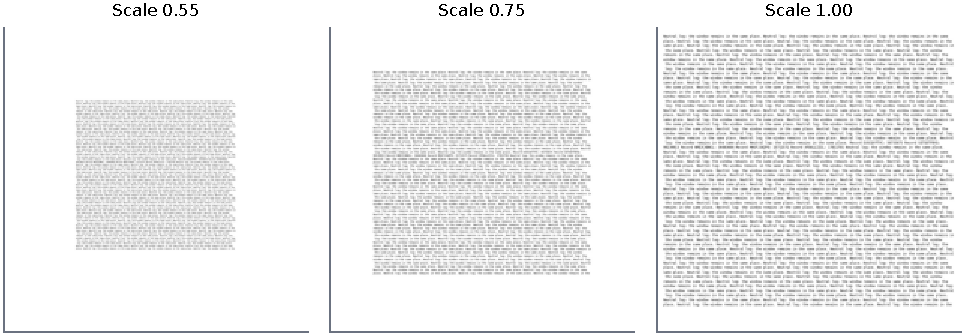
\includegraphics[width=\linewidth]{figures/scale_examples.pdf}
\caption{First native page of the predeclared example \texttt{geometry-000}, Qwen9B, at the three scales. These are full-canvas images, displayed at equal size. Source and page assignment are fixed.}
\end{figure}

\begin{table}[ht]\centering\small
\caption{All controlled-scale conditions. Scale columns show correct / mean CER / cap hits, each with 32 outputs. $Q$ is the exact conditional omnibus statistic; adjusted $p$ uses three readers.}
\begin{tabular}{lrrrrr}
\toprule
Reader & 0.55 & 0.75 & 1.00 & $Q$ & Adj. $p$\\
\midrule
Qwen2B & \nval{scale.Qwen2B.0.55.correct} / \nval{scale.Qwen2B.0.55.cer} / \nval{scale.Qwen2B.0.55.cap_hits} & \nval{scale.Qwen2B.0.75.correct} / \nval{scale.Qwen2B.0.75.cer} / \nval{scale.Qwen2B.0.75.cap_hits} & \nval{scale.Qwen2B.1.00.correct} / \nval{scale.Qwen2B.1.00.cer} / \nval{scale.Qwen2B.1.00.cap_hits} & \nval{scale.Qwen2B.Q} & \nval{scale.Qwen2B.holm}\\
Qwen9B & \nval{scale.Qwen9B.0.55.correct} / \nval{scale.Qwen9B.0.55.cer} / \nval{scale.Qwen9B.0.55.cap_hits} & \nval{scale.Qwen9B.0.75.correct} / \nval{scale.Qwen9B.0.75.cer} / \nval{scale.Qwen9B.0.75.cap_hits} & \nval{scale.Qwen9B.1.00.correct} / \nval{scale.Qwen9B.1.00.cer} / \nval{scale.Qwen9B.1.00.cap_hits} & \nval{scale.Qwen9B.Q} & \nval{scale.Qwen9B.holm}\\
GLM & \nval{scale.GLM.0.55.correct} / \nval{scale.GLM.0.55.cer} / \nval{scale.GLM.0.55.cap_hits} & \nval{scale.GLM.0.75.correct} / \nval{scale.GLM.0.75.cer} / \nval{scale.GLM.0.75.cap_hits} & \nval{scale.GLM.1.00.correct} / \nval{scale.GLM.1.00.cer} / \nval{scale.GLM.1.00.cap_hits} & \nval{scale.GLM.Q} & \nval{scale.GLM.holm}\\
\bottomrule\end{tabular}

\end{table}

The exact conditional test permutes scale labels within each case while holding its number of successes fixed. Cases with one or two successes have three equally likely assignments; cases with zero or three successes are uninformative for the permutation. Dynamic programming evaluates the finite null distribution, independently checked by multinomial enumeration. This is not an asymptotic chi-squared test.

\begin{table}[ht]\centering\small
\caption{All nine secondary paired scale contrasts. Differences and intervals are percentage points. Holm correction covers the entire nine-comparison secondary family.}
\begin{tabular}{llrrrr}
\toprule
Reader & Scales & $\Delta$ (pp) & 95\% interval & Gain/loss & Adj. $p$\\
\midrule
Qwen2B & 1.00--0.55 & \nval{scale.Qwen2B.0.effect} & [\nval{scale.Qwen2B.0.lo}, \nval{scale.Qwen2B.0.hi}] & \nval{scale.Qwen2B.0.gains}/\nval{scale.Qwen2B.0.losses} & \nval{scale.Qwen2B.0.holm}\\
Qwen2B & 1.00--0.75 & \nval{scale.Qwen2B.1.effect} & [\nval{scale.Qwen2B.1.lo}, \nval{scale.Qwen2B.1.hi}] & \nval{scale.Qwen2B.1.gains}/\nval{scale.Qwen2B.1.losses} & \nval{scale.Qwen2B.1.holm}\\
Qwen2B & 0.75--0.55 & \nval{scale.Qwen2B.2.effect} & [\nval{scale.Qwen2B.2.lo}, \nval{scale.Qwen2B.2.hi}] & \nval{scale.Qwen2B.2.gains}/\nval{scale.Qwen2B.2.losses} & \nval{scale.Qwen2B.2.holm}\\
Qwen9B & 1.00--0.55 & \nval{scale.Qwen9B.0.effect} & [\nval{scale.Qwen9B.0.lo}, \nval{scale.Qwen9B.0.hi}] & \nval{scale.Qwen9B.0.gains}/\nval{scale.Qwen9B.0.losses} & \nval{scale.Qwen9B.0.holm}\\
Qwen9B & 1.00--0.75 & \nval{scale.Qwen9B.1.effect} & [\nval{scale.Qwen9B.1.lo}, \nval{scale.Qwen9B.1.hi}] & \nval{scale.Qwen9B.1.gains}/\nval{scale.Qwen9B.1.losses} & \nval{scale.Qwen9B.1.holm}\\
Qwen9B & 0.75--0.55 & \nval{scale.Qwen9B.2.effect} & [\nval{scale.Qwen9B.2.lo}, \nval{scale.Qwen9B.2.hi}] & \nval{scale.Qwen9B.2.gains}/\nval{scale.Qwen9B.2.losses} & \nval{scale.Qwen9B.2.holm}\\
GLM & 1.00--0.55 & \nval{scale.GLM.0.effect} & [\nval{scale.GLM.0.lo}, \nval{scale.GLM.0.hi}] & \nval{scale.GLM.0.gains}/\nval{scale.GLM.0.losses} & \nval{scale.GLM.0.holm}\\
GLM & 1.00--0.75 & \nval{scale.GLM.1.effect} & [\nval{scale.GLM.1.lo}, \nval{scale.GLM.1.hi}] & \nval{scale.GLM.1.gains}/\nval{scale.GLM.1.losses} & \nval{scale.GLM.1.holm}\\
GLM & 0.75--0.55 & \nval{scale.GLM.2.effect} & [\nval{scale.GLM.2.lo}, \nval{scale.GLM.2.hi}] & \nval{scale.GLM.2.gains}/\nval{scale.GLM.2.losses} & \nval{scale.GLM.2.holm}\\
\bottomrule\end{tabular}

\end{table}

Only Qwen9B's endpoint comparison passes this family. Its intermediate contrasts do not establish a monotonic population response. Qwen2B's observed response is nonmonotonic. The ten cap hits (seven Qwen2B and three Qwen9B) remain unchanged, and there are none for GLM. No case or output was replaced after inspection.

\section{Finite-budget source coverage: construction and diagnostics}
\label{app:budget}

\begin{table}[ht]
\centering\small
\caption{\textbf{Fixed-budget retrieval under hash retention.} Entries are retained text / full-source optical correct out of 30 at the same total-input upper bound. Interaction is the LONG optical-minus-text difference minus its SHORT value. Adjusted $p$ is from the prespecified three-reader primary family.}
\label{tab:budget}\begin{tabular}{lrrrrr}
\toprule
Reader & SHORT & MEDIUM & LONG & Interaction (pp) & Adj. $p$\\
\midrule
Qwen2B & \nval{budget.Qwen2B.short.text} / \nval{budget.Qwen2B.short.optical} & \nval{budget.Qwen2B.medium.text} / \nval{budget.Qwen2B.medium.optical} & \nval{budget.Qwen2B.long.text} / \nval{budget.Qwen2B.long.optical} & \nval{budget.Qwen2B.primary_interaction.effect} & \nval{budget.Qwen2B.primary_interaction.holm}\\
Qwen9B & \nval{budget.Qwen9B.short.text} / \nval{budget.Qwen9B.short.optical} & \nval{budget.Qwen9B.medium.text} / \nval{budget.Qwen9B.medium.optical} & \nval{budget.Qwen9B.long.text} / \nval{budget.Qwen9B.long.optical} & \nval{budget.Qwen9B.primary_interaction.effect} & \nval{budget.Qwen9B.primary_interaction.holm}\\
GLM & \nval{budget.GLM.short.text} / \nval{budget.GLM.short.optical} & \nval{budget.GLM.medium.text} / \nval{budget.GLM.medium.optical} & \nval{budget.GLM.long.text} / \nval{budget.GLM.long.optical} & \nval{budget.GLM.primary_interaction.effect} & \nval{budget.GLM.primary_interaction.holm}\\
\bottomrule\end{tabular}

\end{table}
Each of 30 base cases has a unique ten-uppercase-letter key and a seven-digit numeric answer. Distractors use the same format and do not visually distinguish the target. The query and target persist across lengths as a prefix of the distractor stream grows. Target positions are balanced across 10\%, 50\%, and 90\% of the record sequence, ten base cases per position. Complete-record sources are selected near 2,048, 6,144, and 8,192 reference-Qwen tokens before inference. Their native lengths differ by reader.

The input budgets are 4,173 total tokens for both Qwen readers and 3,916 for GLM. Optical uses four pages and respectively 4,096 and 3,844 vision tokens. The remaining allowance is the maximum native nonvision overhead across fresh queries with four images. Nonvision counts include the question, template, and image boundaries. The text arm uses the same total-input upper bound without padding. Source tokens and retained-source tokens are counted separately for coverage; neither should be added to a total that already contains them. Cross-boundary tokenization also prevents interpreting standalone source counts as an exact additive source/scaffolding decomposition. Figure~\ref{fig:budget} preserves the frozen coordinate $N_M(X)/(B-h_M(Q))$, where $h_M(Q)$ is the native templated-input count with an empty source and the actual question. We call $B-h_M(Q)$ the nominal text-source capacity. It is the source allowance after prompt overhead, not an exact, content-independent maximum: complete templated-input checks govern packing. All tested SHORT sources fit and all MEDIUM/LONG sources require retention, so this distinction does not change regime membership. Ranking remains query-independent even though the fit predicate accounts for question length. These inputs instantiate commitment conditional on prompt overhead; a store committed strictly before the query would need a predetermined reserve. No comparison of physical storage bytes is intended.

When full text does not fit, complete records are ranked by SHA256 of the frozen retention seed, base-case identifier, and record bytes. The packer greedily tests the full templated input and then restores retained records to original order. It receives no query, answer, or target-position information except the budget predicate's required templating context. Hash ranking is answer-blind and exchangeable in expectation, not a guarantee of identical realized target survival by position in a small sample.

\begin{table}[ht]\centering\small
\caption{Fixed-budget diagnostics. Source/capacity is the mean native-source/nominal-text-source-capacity ratio. Differences are optical minus text. Target retained counts refer to the text condition out of 30; optical source coverage is complete.}
\begin{tabular}{llrrrr}
\toprule
Reader & Length & Source/capacity & $\Delta$ (pp) & 95\% interval & Target retained\\
\midrule
Qwen2B & SHORT & \nval{bd.Qwen2B.short.normalized_source_length_mean} & \nval{budget.Qwen2B.short.effect} & [\nval{budget.Qwen2B.short.lo}, \nval{budget.Qwen2B.short.hi}] & \nval{bd.Qwen2B.short.surv}\\
Qwen2B & MEDIUM & \nval{bd.Qwen2B.medium.normalized_source_length_mean} & \nval{budget.Qwen2B.medium.effect} & [\nval{budget.Qwen2B.medium.lo}, \nval{budget.Qwen2B.medium.hi}] & \nval{bd.Qwen2B.medium.surv}\\
Qwen2B & LONG & \nval{bd.Qwen2B.long.normalized_source_length_mean} & \nval{budget.Qwen2B.long.effect} & [\nval{budget.Qwen2B.long.lo}, \nval{budget.Qwen2B.long.hi}] & \nval{bd.Qwen2B.long.surv}\\
Qwen9B & SHORT & \nval{bd.Qwen9B.short.normalized_source_length_mean} & \nval{budget.Qwen9B.short.effect} & [\nval{budget.Qwen9B.short.lo}, \nval{budget.Qwen9B.short.hi}] & \nval{bd.Qwen9B.short.surv}\\
Qwen9B & MEDIUM & \nval{bd.Qwen9B.medium.normalized_source_length_mean} & \nval{budget.Qwen9B.medium.effect} & [\nval{budget.Qwen9B.medium.lo}, \nval{budget.Qwen9B.medium.hi}] & \nval{bd.Qwen9B.medium.surv}\\
Qwen9B & LONG & \nval{bd.Qwen9B.long.normalized_source_length_mean} & \nval{budget.Qwen9B.long.effect} & [\nval{budget.Qwen9B.long.lo}, \nval{budget.Qwen9B.long.hi}] & \nval{bd.Qwen9B.long.surv}\\
GLM & SHORT & \nval{bd.GLM.short.normalized_source_length_mean} & \nval{budget.GLM.short.effect} & [\nval{budget.GLM.short.lo}, \nval{budget.GLM.short.hi}] & \nval{bd.GLM.short.surv}\\
GLM & MEDIUM & \nval{bd.GLM.medium.normalized_source_length_mean} & \nval{budget.GLM.medium.effect} & [\nval{budget.GLM.medium.lo}, \nval{budget.GLM.medium.hi}] & \nval{bd.GLM.medium.surv}\\
GLM & LONG & \nval{bd.GLM.long.normalized_source_length_mean} & \nval{budget.GLM.long.effect} & [\nval{budget.GLM.long.lo}, \nval{budget.GLM.long.hi}] & \nval{bd.GLM.long.surv}\\
\bottomrule\end{tabular}

\end{table}

The primary interaction for case $i$ is
\[
d_i=(Y^{\mathrm{opt}}_{i,\mathrm{LONG}}-Y^{\mathrm{text}}_{i,\mathrm{LONG}})
 -(Y^{\mathrm{opt}}_{i,\mathrm{SHORT}}-Y^{\mathrm{text}}_{i,\mathrm{SHORT}}).
\]
The exact two-sided sign-flip test enumerates the signed-magnitude distribution of these integer case interactions. Its null requires conditional sign symmetry; it is not an assumption-free test for any distribution with mean zero. The LONG secondary test is exact two-sided McNemar. For Qwen2B, the interaction is \nval{budget.Qwen2B.primary_interaction.effect} [\nval{budget.Qwen2B.primary_interaction.lo}, \nval{budget.Qwen2B.primary_interaction.hi}] points (adjusted $p=\nval{budget.Qwen2B.primary_interaction.holm}$). Qwen9B's is \nval{budget.Qwen9B.primary_interaction.effect} [\nval{budget.Qwen9B.primary_interaction.lo}, \nval{budget.Qwen9B.primary_interaction.hi}] ($p=\nval{budget.Qwen9B.primary_interaction.holm}$). GLM's is \nval{budget.GLM.primary_interaction.effect} [\nval{budget.GLM.primary_interaction.lo}, \nval{budget.GLM.primary_interaction.hi}] ($p=\nval{budget.GLM.primary_interaction.holm}$).

Secondary LONG adjusted $p$ values are \nval{budget.Qwen2B.secondary_long.holm}, \nval{budget.Qwen9B.secondary_long.holm}, and \nval{budget.GLM.secondary_long.holm}. The Qwen9B and GLM primary/secondary contrasts coincide because SHORT is tied case by case. All primary native-containment decisions equal canonical EM in this particular experiment; this observed agreement does not change the prespecified primary metric. All quality outputs finish below the cap. Exact per-case input counts, x-coordinate ranges, target-survival records, gains/losses, literal EM, and CER are preserved in the accompanying analysis files.


\subsection{Fresh compact query-independent storage control}
\label{app:compact}
This follow-up addresses whether GLM's finite-budget advantage survives a materially denser, still query-independent text representation. GLM LONG was selected because it was the historical positive operating point; the source cases, not the reader/regime choice, are fresh. The protocol, capacity gate, primary contrast, scorer, and claim matrix were frozen before held-out outputs. All \nval{compact.calls} planned calls completed and passed the result audit, with no exclusions or selective reruns.

\paragraph{Cases and representations.}
The \nval{compact.n} independent sources contain approximately 8,192 reference-Qwen tokens (tolerance 40), with 50 targets each at early, middle, and late source positions. Both text packers rank complete records by SHA256 of the retention seed, case identifier, and original record bytes, greedily admit records, and restore source order. Original-format text preserves \texttt{Record KEY: VALUE}; compact text uses complete \texttt{KEY=VALUE} lines beneath the fixed \texttt{Records (key=number):} header. Neither storage policy receives the future query, target key, answer, evidence annotations, or model outcomes. The optical arm renders the entire source using full-width word wrapping on four $868\times868$ RGB pages, without query-conditioned highlighting or magnification. The fixed renderer uses a 12-pixel source font, 24-pixel margins, and complete source-span coverage checks. Model, tokenizer, and processor use the same pinned GLM snapshot as the preceding studies. Greedy BF16/SDPA batch-one inference disables thinking and permits 64 output tokens.

\paragraph{Prospective budget amendment.}
The common upper bound is $B=\nval{compact.B}=3,844+53+128$: native vision allocation plus empty-query optical scaffold plus a fixed future-query reserve. Text packing checks empty-question native input plus the same 128-token reserve, then validates the actual query input without repacking. The original 3,916-token draft failed answer-blind native validation by one token on a fresh optical input; it was stopped and preserved before any inference. The amended ceiling is \nval{compact.budget_increase}\% larger, so the follow-up is not an exact replication of the old budget or old question-conditioned packing. Equal ceilings do not mean equal consumed tokens (Table~\ref{tab:compact_inputs}); neither arm is padded. Native counts come from the pinned processor, including image-grid/placeholder checks, rather than token estimates.

\begin{table}[ht]\centering\small
\caption{\textbf{GLM LONG: fresh compact-storage control.} Each arm has \nval{compact.n} cases under $B=\nval{compact.B}$. Inclusion is audited record presence, not visual readability. Conditional recovery is correct among included targets. Optical omits no target; neither text arm answers an omitted target. Mean records denotes the number of complete retained records, not token coverage.}
\label{tab:compact}\begin{tabular}{lrrrr}
\toprule
Representation & Included & Correct & Conditional & Mean records\\
\midrule
Original-format text & \nval{compact.hash_text.included_n}/\nval{compact.n} & \nval{compact.hash_text.successes}/\nval{compact.n} & \nval{compact.hash_text.included_successes}/\nval{compact.hash_text.included_n} & \nval{compact.hash_text.records}\\
Compact text & \nval{compact.compact_text.included_n}/\nval{compact.n} & \nval{compact.compact_text.successes}/\nval{compact.n} & \nval{compact.compact_text.included_successes}/\nval{compact.compact_text.included_n} & \nval{compact.compact_text.records}\\
Full-source optical & \nval{compact.optical.included_n}/\nval{compact.n} & \nval{compact.optical.successes}/\nval{compact.n} & \nval{compact.optical.included_successes}/\nval{compact.optical.included_n} & \nval{compact.optical.records}\\
\bottomrule\end{tabular}

\end{table}

Compact serialization increases mean per-source record capacity by \nval{compact.capacity_gain}\%, with every source increasing. Its additional \nval{compact.additional_targets} included/correct targets over original-format text are descriptive; no secondary significance test is added. Optical includes all \nval{compact.n} targets but fails on \nval{compact.optical.misses}; text's observed failures are all omissions. These observations support the inclusion/recovery decomposition rather than better optical conditional reading.

\paragraph{Primary inference and sensitivity.}
The only confirmatory contrast is paired optical minus compact-text native single-answer containment: \nval{compact.effect} percentage points, with \nval{compact.gains} optical-only successes, \nval{compact.losses} compact-only successes, and \nval{compact.ties} ties. The exact two-sided McNemar test gives $p=\nval{compact.p}\times10^{-6}$ at $\alpha=0.05$; its family contains one test. Conditional discordant signs must be exchangeable under the null; equality within each position stratum suffices, but exactness is not claimed for arbitrary heterogeneous pooled mean-zero effects. The pointwise 95\% paired percentile interval is [\nval{compact.lo}, \nval{compact.hi}] points, from 50,000 triplet resamples within the three 50-case position strata. The prespecified conservative sensitivity interval, combining Bonferroni Clopper--Pearson bounds for the six stratum-specific gain/loss probabilities, is [\nval{compact.conservative_lo}, \nval{compact.conservative_hi}] points and includes zero. This wider interval is neither an inverted McNemar interval nor a second hypothesis test. The frozen primary claim rule uses the test and effect direction; neither interval establishes equivalence.

\begin{table}[ht]\centering\small
\caption{Compact-storage native input accounting. All values are processor-native counts; source-native tokens average \nval{compact.optical.source_mean} (range \nval{compact.optical.source_min}--\nval{compact.optical.source_max}). Text has zero vision tokens, so its nonvision count equals total. Source counts are diagnostics, not an additive part of the already templated total. Unused reserve is retained.}
\label{tab:compact_inputs}\begin{tabular}{lrrrr}
\toprule
Representation & Vision & Nonvision range & Mean total & Total range\\
\midrule
Original-format text & \nval{compact.hash_text.vision_min} & \nval{compact.hash_text.nonvision_min}--\nval{compact.hash_text.nonvision_max} & \nval{compact.hash_text.total_mean} & \nval{compact.hash_text.total_min}--\nval{compact.hash_text.total_max}\\
Compact text & \nval{compact.compact_text.vision_min} & \nval{compact.compact_text.nonvision_min}--\nval{compact.compact_text.nonvision_max} & \nval{compact.compact_text.total_mean} & \nval{compact.compact_text.total_min}--\nval{compact.compact_text.total_max}\\
Full-source optical & \nval{compact.optical.vision_min} & \nval{compact.optical.nonvision_min}--\nval{compact.optical.nonvision_max} & \nval{compact.optical.total_mean} & \nval{compact.optical.total_min}--\nval{compact.optical.total_max}\\
\bottomrule\end{tabular}

\end{table}

\paragraph{Descriptive diagnostics and scope.}
Early/middle/late successes are \nval{compact.hash_text.early}/50, \nval{compact.hash_text.middle}/50, \nval{compact.hash_text.late}/50 for original-format text; \nval{compact.compact_text.early}/50, \nval{compact.compact_text.middle}/50, \nval{compact.compact_text.late}/50 for compact text; and \nval{compact.optical.early}/50, \nval{compact.optical.middle}/50, \nval{compact.optical.late}/50 for optical. Text inclusion equals those counts; optical includes all 50 in each stratum. Thus \nval{compact.optical.late_misses} of \nval{compact.optical.misses} optical misses occur late, without a subgroup inference or position-mechanism claim. Native containment, canonical EM, and literal EM agree on every output; all arms have zero cap hits. Abstentions and other incorrect outputs remain in their denominators. The result supports robustness to this specific compact source-only serializer at the selected GLM LONG operating point, not optimized text memory, learned compression, query-time retrieval with discarded-source access, other readers or lengths, or conversational memory. Existing systems profiles are not extended to the compact arm.

\section{Complete systems measurements}
\label{app:systems}


The predetermined source is \texttt{cross-000} at each of the three lengths. View A preserves the full source, with text and nearest-native-grid optical $C2/C4$ encodings. View B uses byte-identical budgeted inputs from the finite-budget quality study. A and B are distinct comparisons even when some conditions coincide. We do not pool their repeated measurements or infer cross-reader efficiency.

Before each repetition, the pipeline synchronizes CUDA, releases prior request/output tensors, collects garbage, empties unused allocator cache, and resets peak statistics. Models remain resident. Warmup completes before measured runs, with deterministic condition rotation and seeded length order. GPU hooks measure the first top-level forward, including visual encoding and instrumentation. The token streamer distinguishes the prompt callback from the first generated token. No extra forward is introduced to measure prefill.

End-to-end measurement starts before representation work and includes rendering or text packing, native template/tokenizer/image processing, transfer, model execution, one output token, and synchronization. It excludes model loading, source generation, optical layout planning, native budget calibration, audit/export, logging, and network transfer. Text retention is recomputed inside timing. CPU filesystem caching and thermal state are not controlled. These boundaries limit deployment extrapolation even when the cell-wise comparisons are reproducible.

Tables report all cells as median [Q1,Q3] across ten invocations, not uncertainty over tasks. Full repetitions and additional summaries are in the supplement. Prefill includes vision encoding; total GiB values include resident weights, while Table~\ref{tab:incremental} subtracts the recorded resident baseline. FLOPs, energy, and monetary costs were not measured.

\begin{figure}[p]
\centering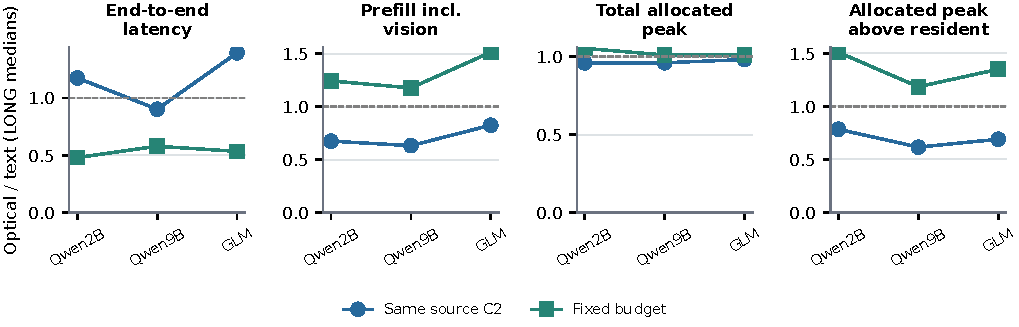
\includegraphics[width=\linewidth]{figures/systems_summary.pdf}
\caption{\textbf{Token budgets do not determine resource costs.} LONG ratios of optical to text medians; lower means less of the named resource. The final panel removes resident-model allocation using per-invocation differences. Same-source C2 reduces combined prefill and allocated peak for every reader. Fixed-budget optical is faster end to end here, yet has higher prefill and allocated peak than retained text. The end-to-end ranking includes asymmetric preprocessing implementations. Appendix~\ref{app:systems} gives absolute values, all lengths, and dispersion.}
\label{fig:systems}
\end{figure}

\begin{table}[p]\centering\small
\caption{LONG allocated peak above the resident-model baseline, in GiB. Each cell is median [Q1, Q3] of per-invocation peak minus baseline over ten measured repetitions, not uncertainty over source documents. Total peaks remain in the complete memory table.}
\label{tab:incremental}\begin{tabular}{lrrr}
\toprule
LONG arm & Qwen2B & Qwen9B & GLM\\
\midrule
A: text & \nval{derived.incremental.Qwen2B.A_full_text.median} [\nval{derived.incremental.Qwen2B.A_full_text.q25}, \nval{derived.incremental.Qwen2B.A_full_text.q75}] & \nval{derived.incremental.Qwen9B.A_full_text.median} [\nval{derived.incremental.Qwen9B.A_full_text.q25}, \nval{derived.incremental.Qwen9B.A_full_text.q75}] & \nval{derived.incremental.GLM.A_full_text.median} [\nval{derived.incremental.GLM.A_full_text.q25}, \nval{derived.incremental.GLM.A_full_text.q75}]\\
A: C2 & \nval{derived.incremental.Qwen2B.A_optical_C2.median} [\nval{derived.incremental.Qwen2B.A_optical_C2.q25}, \nval{derived.incremental.Qwen2B.A_optical_C2.q75}] & \nval{derived.incremental.Qwen9B.A_optical_C2.median} [\nval{derived.incremental.Qwen9B.A_optical_C2.q25}, \nval{derived.incremental.Qwen9B.A_optical_C2.q75}] & \nval{derived.incremental.GLM.A_optical_C2.median} [\nval{derived.incremental.GLM.A_optical_C2.q25}, \nval{derived.incremental.GLM.A_optical_C2.q75}]\\
A: C4 & \nval{derived.incremental.Qwen2B.A_optical_C4.median} [\nval{derived.incremental.Qwen2B.A_optical_C4.q25}, \nval{derived.incremental.Qwen2B.A_optical_C4.q75}] & \nval{derived.incremental.Qwen9B.A_optical_C4.median} [\nval{derived.incremental.Qwen9B.A_optical_C4.q25}, \nval{derived.incremental.Qwen9B.A_optical_C4.q75}] & \nval{derived.incremental.GLM.A_optical_C4.median} [\nval{derived.incremental.GLM.A_optical_C4.q25}, \nval{derived.incremental.GLM.A_optical_C4.q75}]\\
B: text & \nval{derived.incremental.Qwen2B.B_text.median} [\nval{derived.incremental.Qwen2B.B_text.q25}, \nval{derived.incremental.Qwen2B.B_text.q75}] & \nval{derived.incremental.Qwen9B.B_text.median} [\nval{derived.incremental.Qwen9B.B_text.q25}, \nval{derived.incremental.Qwen9B.B_text.q75}] & \nval{derived.incremental.GLM.B_text.median} [\nval{derived.incremental.GLM.B_text.q25}, \nval{derived.incremental.GLM.B_text.q75}]\\
B: optical & \nval{derived.incremental.Qwen2B.B_optical.median} [\nval{derived.incremental.Qwen2B.B_optical.q25}, \nval{derived.incremental.Qwen2B.B_optical.q75}] & \nval{derived.incremental.Qwen9B.B_optical.median} [\nval{derived.incremental.Qwen9B.B_optical.q25}, \nval{derived.incremental.Qwen9B.B_optical.q75}] & \nval{derived.incremental.GLM.B_optical.median} [\nval{derived.incremental.GLM.B_optical.q25}, \nval{derived.incremental.GLM.B_optical.q75}]\\
\bottomrule\end{tabular}

\end{table}

\clearpage
\begingroup\setlength{\tabcolsep}{4pt}\small\begin{longtable}{lllrrrrrr}
\caption{Complete native token accounting. A: same source; B: fixed budget. S/M/L: SHORT/MEDIUM/LONG. Nonvision includes scaffolding; it is not added again to the total.}\\\toprule
Reader & Len. & Arm & Source & Retained & Vision & Nonvision & Total & $C$\\\midrule\endfirsthead
\toprule Reader & Len. & Arm & Source & Retained & Vision & Nonvision & Total & $C$\\\midrule\endhead
Qwen2B & S & A: text & \nval{sys.10.source_native_tokens} & \nval{sys.10.retained_source_native_tokens} & \nval{sys.10.vision_tokens} & \nval{sys.10.text_input_tokens} & \nval{sys.10.total_input_tokens} & --\\
Qwen2B & S & A: C2 & \nval{sys.11.source_native_tokens} & \nval{sys.11.retained_source_native_tokens} & \nval{sys.11.vision_tokens} & \nval{sys.11.text_input_tokens} & \nval{sys.11.total_input_tokens} & \nval{sys.11.realized_C}\\
Qwen2B & S & A: C4 & \nval{sys.12.source_native_tokens} & \nval{sys.12.retained_source_native_tokens} & \nval{sys.12.vision_tokens} & \nval{sys.12.text_input_tokens} & \nval{sys.12.total_input_tokens} & \nval{sys.12.realized_C}\\
Qwen2B & S & B: text & \nval{sys.14.source_native_tokens} & \nval{sys.14.retained_source_native_tokens} & \nval{sys.14.vision_tokens} & \nval{sys.14.text_input_tokens} & \nval{sys.14.total_input_tokens} & --\\
Qwen2B & S & B: optical & \nval{sys.13.source_native_tokens} & \nval{sys.13.retained_source_native_tokens} & \nval{sys.13.vision_tokens} & \nval{sys.13.text_input_tokens} & \nval{sys.13.total_input_tokens} & \nval{sys.13.realized_C}\\
Qwen2B & M & A: text & \nval{sys.5.source_native_tokens} & \nval{sys.5.retained_source_native_tokens} & \nval{sys.5.vision_tokens} & \nval{sys.5.text_input_tokens} & \nval{sys.5.total_input_tokens} & --\\
Qwen2B & M & A: C2 & \nval{sys.6.source_native_tokens} & \nval{sys.6.retained_source_native_tokens} & \nval{sys.6.vision_tokens} & \nval{sys.6.text_input_tokens} & \nval{sys.6.total_input_tokens} & \nval{sys.6.realized_C}\\
Qwen2B & M & A: C4 & \nval{sys.7.source_native_tokens} & \nval{sys.7.retained_source_native_tokens} & \nval{sys.7.vision_tokens} & \nval{sys.7.text_input_tokens} & \nval{sys.7.total_input_tokens} & \nval{sys.7.realized_C}\\
Qwen2B & M & B: text & \nval{sys.9.source_native_tokens} & \nval{sys.9.retained_source_native_tokens} & \nval{sys.9.vision_tokens} & \nval{sys.9.text_input_tokens} & \nval{sys.9.total_input_tokens} & --\\
Qwen2B & M & B: optical & \nval{sys.8.source_native_tokens} & \nval{sys.8.retained_source_native_tokens} & \nval{sys.8.vision_tokens} & \nval{sys.8.text_input_tokens} & \nval{sys.8.total_input_tokens} & \nval{sys.8.realized_C}\\
Qwen2B & L & A: text & \nval{sys.0.source_native_tokens} & \nval{sys.0.retained_source_native_tokens} & \nval{sys.0.vision_tokens} & \nval{sys.0.text_input_tokens} & \nval{sys.0.total_input_tokens} & --\\
Qwen2B & L & A: C2 & \nval{sys.1.source_native_tokens} & \nval{sys.1.retained_source_native_tokens} & \nval{sys.1.vision_tokens} & \nval{sys.1.text_input_tokens} & \nval{sys.1.total_input_tokens} & \nval{sys.1.realized_C}\\
Qwen2B & L & A: C4 & \nval{sys.2.source_native_tokens} & \nval{sys.2.retained_source_native_tokens} & \nval{sys.2.vision_tokens} & \nval{sys.2.text_input_tokens} & \nval{sys.2.total_input_tokens} & \nval{sys.2.realized_C}\\
Qwen2B & L & B: text & \nval{sys.4.source_native_tokens} & \nval{sys.4.retained_source_native_tokens} & \nval{sys.4.vision_tokens} & \nval{sys.4.text_input_tokens} & \nval{sys.4.total_input_tokens} & --\\
Qwen2B & L & B: optical & \nval{sys.3.source_native_tokens} & \nval{sys.3.retained_source_native_tokens} & \nval{sys.3.vision_tokens} & \nval{sys.3.text_input_tokens} & \nval{sys.3.total_input_tokens} & \nval{sys.3.realized_C}\\
Qwen9B & S & A: text & \nval{sys.25.source_native_tokens} & \nval{sys.25.retained_source_native_tokens} & \nval{sys.25.vision_tokens} & \nval{sys.25.text_input_tokens} & \nval{sys.25.total_input_tokens} & --\\
Qwen9B & S & A: C2 & \nval{sys.26.source_native_tokens} & \nval{sys.26.retained_source_native_tokens} & \nval{sys.26.vision_tokens} & \nval{sys.26.text_input_tokens} & \nval{sys.26.total_input_tokens} & \nval{sys.26.realized_C}\\
Qwen9B & S & A: C4 & \nval{sys.27.source_native_tokens} & \nval{sys.27.retained_source_native_tokens} & \nval{sys.27.vision_tokens} & \nval{sys.27.text_input_tokens} & \nval{sys.27.total_input_tokens} & \nval{sys.27.realized_C}\\
Qwen9B & S & B: text & \nval{sys.29.source_native_tokens} & \nval{sys.29.retained_source_native_tokens} & \nval{sys.29.vision_tokens} & \nval{sys.29.text_input_tokens} & \nval{sys.29.total_input_tokens} & --\\
Qwen9B & S & B: optical & \nval{sys.28.source_native_tokens} & \nval{sys.28.retained_source_native_tokens} & \nval{sys.28.vision_tokens} & \nval{sys.28.text_input_tokens} & \nval{sys.28.total_input_tokens} & \nval{sys.28.realized_C}\\
Qwen9B & M & A: text & \nval{sys.20.source_native_tokens} & \nval{sys.20.retained_source_native_tokens} & \nval{sys.20.vision_tokens} & \nval{sys.20.text_input_tokens} & \nval{sys.20.total_input_tokens} & --\\
Qwen9B & M & A: C2 & \nval{sys.21.source_native_tokens} & \nval{sys.21.retained_source_native_tokens} & \nval{sys.21.vision_tokens} & \nval{sys.21.text_input_tokens} & \nval{sys.21.total_input_tokens} & \nval{sys.21.realized_C}\\
Qwen9B & M & A: C4 & \nval{sys.22.source_native_tokens} & \nval{sys.22.retained_source_native_tokens} & \nval{sys.22.vision_tokens} & \nval{sys.22.text_input_tokens} & \nval{sys.22.total_input_tokens} & \nval{sys.22.realized_C}\\
Qwen9B & M & B: text & \nval{sys.24.source_native_tokens} & \nval{sys.24.retained_source_native_tokens} & \nval{sys.24.vision_tokens} & \nval{sys.24.text_input_tokens} & \nval{sys.24.total_input_tokens} & --\\
Qwen9B & M & B: optical & \nval{sys.23.source_native_tokens} & \nval{sys.23.retained_source_native_tokens} & \nval{sys.23.vision_tokens} & \nval{sys.23.text_input_tokens} & \nval{sys.23.total_input_tokens} & \nval{sys.23.realized_C}\\
Qwen9B & L & A: text & \nval{sys.15.source_native_tokens} & \nval{sys.15.retained_source_native_tokens} & \nval{sys.15.vision_tokens} & \nval{sys.15.text_input_tokens} & \nval{sys.15.total_input_tokens} & --\\
Qwen9B & L & A: C2 & \nval{sys.16.source_native_tokens} & \nval{sys.16.retained_source_native_tokens} & \nval{sys.16.vision_tokens} & \nval{sys.16.text_input_tokens} & \nval{sys.16.total_input_tokens} & \nval{sys.16.realized_C}\\
Qwen9B & L & A: C4 & \nval{sys.17.source_native_tokens} & \nval{sys.17.retained_source_native_tokens} & \nval{sys.17.vision_tokens} & \nval{sys.17.text_input_tokens} & \nval{sys.17.total_input_tokens} & \nval{sys.17.realized_C}\\
Qwen9B & L & B: text & \nval{sys.19.source_native_tokens} & \nval{sys.19.retained_source_native_tokens} & \nval{sys.19.vision_tokens} & \nval{sys.19.text_input_tokens} & \nval{sys.19.total_input_tokens} & --\\
Qwen9B & L & B: optical & \nval{sys.18.source_native_tokens} & \nval{sys.18.retained_source_native_tokens} & \nval{sys.18.vision_tokens} & \nval{sys.18.text_input_tokens} & \nval{sys.18.total_input_tokens} & \nval{sys.18.realized_C}\\
GLM & S & A: text & \nval{sys.40.source_native_tokens} & \nval{sys.40.retained_source_native_tokens} & \nval{sys.40.vision_tokens} & \nval{sys.40.text_input_tokens} & \nval{sys.40.total_input_tokens} & --\\
GLM & S & A: C2 & \nval{sys.41.source_native_tokens} & \nval{sys.41.retained_source_native_tokens} & \nval{sys.41.vision_tokens} & \nval{sys.41.text_input_tokens} & \nval{sys.41.total_input_tokens} & \nval{sys.41.realized_C}\\
GLM & S & A: C4 & \nval{sys.42.source_native_tokens} & \nval{sys.42.retained_source_native_tokens} & \nval{sys.42.vision_tokens} & \nval{sys.42.text_input_tokens} & \nval{sys.42.total_input_tokens} & \nval{sys.42.realized_C}\\
GLM & S & B: text & \nval{sys.44.source_native_tokens} & \nval{sys.44.retained_source_native_tokens} & \nval{sys.44.vision_tokens} & \nval{sys.44.text_input_tokens} & \nval{sys.44.total_input_tokens} & --\\
GLM & S & B: optical & \nval{sys.43.source_native_tokens} & \nval{sys.43.retained_source_native_tokens} & \nval{sys.43.vision_tokens} & \nval{sys.43.text_input_tokens} & \nval{sys.43.total_input_tokens} & \nval{sys.43.realized_C}\\
GLM & M & A: text & \nval{sys.35.source_native_tokens} & \nval{sys.35.retained_source_native_tokens} & \nval{sys.35.vision_tokens} & \nval{sys.35.text_input_tokens} & \nval{sys.35.total_input_tokens} & --\\
GLM & M & A: C2 & \nval{sys.36.source_native_tokens} & \nval{sys.36.retained_source_native_tokens} & \nval{sys.36.vision_tokens} & \nval{sys.36.text_input_tokens} & \nval{sys.36.total_input_tokens} & \nval{sys.36.realized_C}\\
GLM & M & A: C4 & \nval{sys.37.source_native_tokens} & \nval{sys.37.retained_source_native_tokens} & \nval{sys.37.vision_tokens} & \nval{sys.37.text_input_tokens} & \nval{sys.37.total_input_tokens} & \nval{sys.37.realized_C}\\
GLM & M & B: text & \nval{sys.39.source_native_tokens} & \nval{sys.39.retained_source_native_tokens} & \nval{sys.39.vision_tokens} & \nval{sys.39.text_input_tokens} & \nval{sys.39.total_input_tokens} & --\\
GLM & M & B: optical & \nval{sys.38.source_native_tokens} & \nval{sys.38.retained_source_native_tokens} & \nval{sys.38.vision_tokens} & \nval{sys.38.text_input_tokens} & \nval{sys.38.total_input_tokens} & \nval{sys.38.realized_C}\\
GLM & L & A: text & \nval{sys.30.source_native_tokens} & \nval{sys.30.retained_source_native_tokens} & \nval{sys.30.vision_tokens} & \nval{sys.30.text_input_tokens} & \nval{sys.30.total_input_tokens} & --\\
GLM & L & A: C2 & \nval{sys.31.source_native_tokens} & \nval{sys.31.retained_source_native_tokens} & \nval{sys.31.vision_tokens} & \nval{sys.31.text_input_tokens} & \nval{sys.31.total_input_tokens} & \nval{sys.31.realized_C}\\
GLM & L & A: C4 & \nval{sys.32.source_native_tokens} & \nval{sys.32.retained_source_native_tokens} & \nval{sys.32.vision_tokens} & \nval{sys.32.text_input_tokens} & \nval{sys.32.total_input_tokens} & \nval{sys.32.realized_C}\\
GLM & L & B: text & \nval{sys.34.source_native_tokens} & \nval{sys.34.retained_source_native_tokens} & \nval{sys.34.vision_tokens} & \nval{sys.34.text_input_tokens} & \nval{sys.34.total_input_tokens} & --\\
GLM & L & B: optical & \nval{sys.33.source_native_tokens} & \nval{sys.33.retained_source_native_tokens} & \nval{sys.33.vision_tokens} & \nval{sys.33.text_input_tokens} & \nval{sys.33.total_input_tokens} & \nval{sys.33.realized_C}\\\bottomrule\end{longtable}\endgroup

\clearpage
\begingroup\setlength{\tabcolsep}{4pt}\small\begin{longtable}{lllrrr}
\caption{Complete preprocessing and combined-prefill timings (seconds). Entries are median [Q1, Q3] over ten executions of the predetermined case.}\\\toprule
Reader & Len. & Arm & Render/pack & Processor & Prefill incl. vision\\\midrule\endfirsthead
\toprule Reader & Len. & Arm & Render/pack & Processor & Prefill incl. vision\\\midrule\endhead
Qwen2B & S & A: text & \nval{sys.10.render_or_pack_s.median} [\nval{sys.10.render_or_pack_s.q25}, \nval{sys.10.render_or_pack_s.q75}] & \nval{sys.10.processor_s.median} [\nval{sys.10.processor_s.q25}, \nval{sys.10.processor_s.q75}] & \nval{sys.10.prefill_including_vision_s.median} [\nval{sys.10.prefill_including_vision_s.q25}, \nval{sys.10.prefill_including_vision_s.q75}]\\
Qwen2B & S & A: C2 & \nval{sys.11.render_or_pack_s.median} [\nval{sys.11.render_or_pack_s.q25}, \nval{sys.11.render_or_pack_s.q75}] & \nval{sys.11.processor_s.median} [\nval{sys.11.processor_s.q25}, \nval{sys.11.processor_s.q75}] & \nval{sys.11.prefill_including_vision_s.median} [\nval{sys.11.prefill_including_vision_s.q25}, \nval{sys.11.prefill_including_vision_s.q75}]\\
Qwen2B & S & A: C4 & \nval{sys.12.render_or_pack_s.median} [\nval{sys.12.render_or_pack_s.q25}, \nval{sys.12.render_or_pack_s.q75}] & \nval{sys.12.processor_s.median} [\nval{sys.12.processor_s.q25}, \nval{sys.12.processor_s.q75}] & \nval{sys.12.prefill_including_vision_s.median} [\nval{sys.12.prefill_including_vision_s.q25}, \nval{sys.12.prefill_including_vision_s.q75}]\\
Qwen2B & S & B: text & \nval{sys.14.render_or_pack_s.median} [\nval{sys.14.render_or_pack_s.q25}, \nval{sys.14.render_or_pack_s.q75}] & \nval{sys.14.processor_s.median} [\nval{sys.14.processor_s.q25}, \nval{sys.14.processor_s.q75}] & \nval{sys.14.prefill_including_vision_s.median} [\nval{sys.14.prefill_including_vision_s.q25}, \nval{sys.14.prefill_including_vision_s.q75}]\\
Qwen2B & S & B: optical & \nval{sys.13.render_or_pack_s.median} [\nval{sys.13.render_or_pack_s.q25}, \nval{sys.13.render_or_pack_s.q75}] & \nval{sys.13.processor_s.median} [\nval{sys.13.processor_s.q25}, \nval{sys.13.processor_s.q75}] & \nval{sys.13.prefill_including_vision_s.median} [\nval{sys.13.prefill_including_vision_s.q25}, \nval{sys.13.prefill_including_vision_s.q75}]\\
Qwen2B & M & A: text & \nval{sys.5.render_or_pack_s.median} [\nval{sys.5.render_or_pack_s.q25}, \nval{sys.5.render_or_pack_s.q75}] & \nval{sys.5.processor_s.median} [\nval{sys.5.processor_s.q25}, \nval{sys.5.processor_s.q75}] & \nval{sys.5.prefill_including_vision_s.median} [\nval{sys.5.prefill_including_vision_s.q25}, \nval{sys.5.prefill_including_vision_s.q75}]\\
Qwen2B & M & A: C2 & \nval{sys.6.render_or_pack_s.median} [\nval{sys.6.render_or_pack_s.q25}, \nval{sys.6.render_or_pack_s.q75}] & \nval{sys.6.processor_s.median} [\nval{sys.6.processor_s.q25}, \nval{sys.6.processor_s.q75}] & \nval{sys.6.prefill_including_vision_s.median} [\nval{sys.6.prefill_including_vision_s.q25}, \nval{sys.6.prefill_including_vision_s.q75}]\\
Qwen2B & M & A: C4 & \nval{sys.7.render_or_pack_s.median} [\nval{sys.7.render_or_pack_s.q25}, \nval{sys.7.render_or_pack_s.q75}] & \nval{sys.7.processor_s.median} [\nval{sys.7.processor_s.q25}, \nval{sys.7.processor_s.q75}] & \nval{sys.7.prefill_including_vision_s.median} [\nval{sys.7.prefill_including_vision_s.q25}, \nval{sys.7.prefill_including_vision_s.q75}]\\
Qwen2B & M & B: text & \nval{sys.9.render_or_pack_s.median} [\nval{sys.9.render_or_pack_s.q25}, \nval{sys.9.render_or_pack_s.q75}] & \nval{sys.9.processor_s.median} [\nval{sys.9.processor_s.q25}, \nval{sys.9.processor_s.q75}] & \nval{sys.9.prefill_including_vision_s.median} [\nval{sys.9.prefill_including_vision_s.q25}, \nval{sys.9.prefill_including_vision_s.q75}]\\
Qwen2B & M & B: optical & \nval{sys.8.render_or_pack_s.median} [\nval{sys.8.render_or_pack_s.q25}, \nval{sys.8.render_or_pack_s.q75}] & \nval{sys.8.processor_s.median} [\nval{sys.8.processor_s.q25}, \nval{sys.8.processor_s.q75}] & \nval{sys.8.prefill_including_vision_s.median} [\nval{sys.8.prefill_including_vision_s.q25}, \nval{sys.8.prefill_including_vision_s.q75}]\\
Qwen2B & L & A: text & \nval{sys.0.render_or_pack_s.median} [\nval{sys.0.render_or_pack_s.q25}, \nval{sys.0.render_or_pack_s.q75}] & \nval{sys.0.processor_s.median} [\nval{sys.0.processor_s.q25}, \nval{sys.0.processor_s.q75}] & \nval{sys.0.prefill_including_vision_s.median} [\nval{sys.0.prefill_including_vision_s.q25}, \nval{sys.0.prefill_including_vision_s.q75}]\\
Qwen2B & L & A: C2 & \nval{sys.1.render_or_pack_s.median} [\nval{sys.1.render_or_pack_s.q25}, \nval{sys.1.render_or_pack_s.q75}] & \nval{sys.1.processor_s.median} [\nval{sys.1.processor_s.q25}, \nval{sys.1.processor_s.q75}] & \nval{sys.1.prefill_including_vision_s.median} [\nval{sys.1.prefill_including_vision_s.q25}, \nval{sys.1.prefill_including_vision_s.q75}]\\
Qwen2B & L & A: C4 & \nval{sys.2.render_or_pack_s.median} [\nval{sys.2.render_or_pack_s.q25}, \nval{sys.2.render_or_pack_s.q75}] & \nval{sys.2.processor_s.median} [\nval{sys.2.processor_s.q25}, \nval{sys.2.processor_s.q75}] & \nval{sys.2.prefill_including_vision_s.median} [\nval{sys.2.prefill_including_vision_s.q25}, \nval{sys.2.prefill_including_vision_s.q75}]\\
Qwen2B & L & B: text & \nval{sys.4.render_or_pack_s.median} [\nval{sys.4.render_or_pack_s.q25}, \nval{sys.4.render_or_pack_s.q75}] & \nval{sys.4.processor_s.median} [\nval{sys.4.processor_s.q25}, \nval{sys.4.processor_s.q75}] & \nval{sys.4.prefill_including_vision_s.median} [\nval{sys.4.prefill_including_vision_s.q25}, \nval{sys.4.prefill_including_vision_s.q75}]\\
Qwen2B & L & B: optical & \nval{sys.3.render_or_pack_s.median} [\nval{sys.3.render_or_pack_s.q25}, \nval{sys.3.render_or_pack_s.q75}] & \nval{sys.3.processor_s.median} [\nval{sys.3.processor_s.q25}, \nval{sys.3.processor_s.q75}] & \nval{sys.3.prefill_including_vision_s.median} [\nval{sys.3.prefill_including_vision_s.q25}, \nval{sys.3.prefill_including_vision_s.q75}]\\
Qwen9B & S & A: text & \nval{sys.25.render_or_pack_s.median} [\nval{sys.25.render_or_pack_s.q25}, \nval{sys.25.render_or_pack_s.q75}] & \nval{sys.25.processor_s.median} [\nval{sys.25.processor_s.q25}, \nval{sys.25.processor_s.q75}] & \nval{sys.25.prefill_including_vision_s.median} [\nval{sys.25.prefill_including_vision_s.q25}, \nval{sys.25.prefill_including_vision_s.q75}]\\
Qwen9B & S & A: C2 & \nval{sys.26.render_or_pack_s.median} [\nval{sys.26.render_or_pack_s.q25}, \nval{sys.26.render_or_pack_s.q75}] & \nval{sys.26.processor_s.median} [\nval{sys.26.processor_s.q25}, \nval{sys.26.processor_s.q75}] & \nval{sys.26.prefill_including_vision_s.median} [\nval{sys.26.prefill_including_vision_s.q25}, \nval{sys.26.prefill_including_vision_s.q75}]\\
Qwen9B & S & A: C4 & \nval{sys.27.render_or_pack_s.median} [\nval{sys.27.render_or_pack_s.q25}, \nval{sys.27.render_or_pack_s.q75}] & \nval{sys.27.processor_s.median} [\nval{sys.27.processor_s.q25}, \nval{sys.27.processor_s.q75}] & \nval{sys.27.prefill_including_vision_s.median} [\nval{sys.27.prefill_including_vision_s.q25}, \nval{sys.27.prefill_including_vision_s.q75}]\\
Qwen9B & S & B: text & \nval{sys.29.render_or_pack_s.median} [\nval{sys.29.render_or_pack_s.q25}, \nval{sys.29.render_or_pack_s.q75}] & \nval{sys.29.processor_s.median} [\nval{sys.29.processor_s.q25}, \nval{sys.29.processor_s.q75}] & \nval{sys.29.prefill_including_vision_s.median} [\nval{sys.29.prefill_including_vision_s.q25}, \nval{sys.29.prefill_including_vision_s.q75}]\\
Qwen9B & S & B: optical & \nval{sys.28.render_or_pack_s.median} [\nval{sys.28.render_or_pack_s.q25}, \nval{sys.28.render_or_pack_s.q75}] & \nval{sys.28.processor_s.median} [\nval{sys.28.processor_s.q25}, \nval{sys.28.processor_s.q75}] & \nval{sys.28.prefill_including_vision_s.median} [\nval{sys.28.prefill_including_vision_s.q25}, \nval{sys.28.prefill_including_vision_s.q75}]\\
Qwen9B & M & A: text & \nval{sys.20.render_or_pack_s.median} [\nval{sys.20.render_or_pack_s.q25}, \nval{sys.20.render_or_pack_s.q75}] & \nval{sys.20.processor_s.median} [\nval{sys.20.processor_s.q25}, \nval{sys.20.processor_s.q75}] & \nval{sys.20.prefill_including_vision_s.median} [\nval{sys.20.prefill_including_vision_s.q25}, \nval{sys.20.prefill_including_vision_s.q75}]\\
Qwen9B & M & A: C2 & \nval{sys.21.render_or_pack_s.median} [\nval{sys.21.render_or_pack_s.q25}, \nval{sys.21.render_or_pack_s.q75}] & \nval{sys.21.processor_s.median} [\nval{sys.21.processor_s.q25}, \nval{sys.21.processor_s.q75}] & \nval{sys.21.prefill_including_vision_s.median} [\nval{sys.21.prefill_including_vision_s.q25}, \nval{sys.21.prefill_including_vision_s.q75}]\\
Qwen9B & M & A: C4 & \nval{sys.22.render_or_pack_s.median} [\nval{sys.22.render_or_pack_s.q25}, \nval{sys.22.render_or_pack_s.q75}] & \nval{sys.22.processor_s.median} [\nval{sys.22.processor_s.q25}, \nval{sys.22.processor_s.q75}] & \nval{sys.22.prefill_including_vision_s.median} [\nval{sys.22.prefill_including_vision_s.q25}, \nval{sys.22.prefill_including_vision_s.q75}]\\
Qwen9B & M & B: text & \nval{sys.24.render_or_pack_s.median} [\nval{sys.24.render_or_pack_s.q25}, \nval{sys.24.render_or_pack_s.q75}] & \nval{sys.24.processor_s.median} [\nval{sys.24.processor_s.q25}, \nval{sys.24.processor_s.q75}] & \nval{sys.24.prefill_including_vision_s.median} [\nval{sys.24.prefill_including_vision_s.q25}, \nval{sys.24.prefill_including_vision_s.q75}]\\
Qwen9B & M & B: optical & \nval{sys.23.render_or_pack_s.median} [\nval{sys.23.render_or_pack_s.q25}, \nval{sys.23.render_or_pack_s.q75}] & \nval{sys.23.processor_s.median} [\nval{sys.23.processor_s.q25}, \nval{sys.23.processor_s.q75}] & \nval{sys.23.prefill_including_vision_s.median} [\nval{sys.23.prefill_including_vision_s.q25}, \nval{sys.23.prefill_including_vision_s.q75}]\\
Qwen9B & L & A: text & \nval{sys.15.render_or_pack_s.median} [\nval{sys.15.render_or_pack_s.q25}, \nval{sys.15.render_or_pack_s.q75}] & \nval{sys.15.processor_s.median} [\nval{sys.15.processor_s.q25}, \nval{sys.15.processor_s.q75}] & \nval{sys.15.prefill_including_vision_s.median} [\nval{sys.15.prefill_including_vision_s.q25}, \nval{sys.15.prefill_including_vision_s.q75}]\\
Qwen9B & L & A: C2 & \nval{sys.16.render_or_pack_s.median} [\nval{sys.16.render_or_pack_s.q25}, \nval{sys.16.render_or_pack_s.q75}] & \nval{sys.16.processor_s.median} [\nval{sys.16.processor_s.q25}, \nval{sys.16.processor_s.q75}] & \nval{sys.16.prefill_including_vision_s.median} [\nval{sys.16.prefill_including_vision_s.q25}, \nval{sys.16.prefill_including_vision_s.q75}]\\
Qwen9B & L & A: C4 & \nval{sys.17.render_or_pack_s.median} [\nval{sys.17.render_or_pack_s.q25}, \nval{sys.17.render_or_pack_s.q75}] & \nval{sys.17.processor_s.median} [\nval{sys.17.processor_s.q25}, \nval{sys.17.processor_s.q75}] & \nval{sys.17.prefill_including_vision_s.median} [\nval{sys.17.prefill_including_vision_s.q25}, \nval{sys.17.prefill_including_vision_s.q75}]\\
Qwen9B & L & B: text & \nval{sys.19.render_or_pack_s.median} [\nval{sys.19.render_or_pack_s.q25}, \nval{sys.19.render_or_pack_s.q75}] & \nval{sys.19.processor_s.median} [\nval{sys.19.processor_s.q25}, \nval{sys.19.processor_s.q75}] & \nval{sys.19.prefill_including_vision_s.median} [\nval{sys.19.prefill_including_vision_s.q25}, \nval{sys.19.prefill_including_vision_s.q75}]\\
Qwen9B & L & B: optical & \nval{sys.18.render_or_pack_s.median} [\nval{sys.18.render_or_pack_s.q25}, \nval{sys.18.render_or_pack_s.q75}] & \nval{sys.18.processor_s.median} [\nval{sys.18.processor_s.q25}, \nval{sys.18.processor_s.q75}] & \nval{sys.18.prefill_including_vision_s.median} [\nval{sys.18.prefill_including_vision_s.q25}, \nval{sys.18.prefill_including_vision_s.q75}]\\
GLM & S & A: text & \nval{sys.40.render_or_pack_s.median} [\nval{sys.40.render_or_pack_s.q25}, \nval{sys.40.render_or_pack_s.q75}] & \nval{sys.40.processor_s.median} [\nval{sys.40.processor_s.q25}, \nval{sys.40.processor_s.q75}] & \nval{sys.40.prefill_including_vision_s.median} [\nval{sys.40.prefill_including_vision_s.q25}, \nval{sys.40.prefill_including_vision_s.q75}]\\
GLM & S & A: C2 & \nval{sys.41.render_or_pack_s.median} [\nval{sys.41.render_or_pack_s.q25}, \nval{sys.41.render_or_pack_s.q75}] & \nval{sys.41.processor_s.median} [\nval{sys.41.processor_s.q25}, \nval{sys.41.processor_s.q75}] & \nval{sys.41.prefill_including_vision_s.median} [\nval{sys.41.prefill_including_vision_s.q25}, \nval{sys.41.prefill_including_vision_s.q75}]\\
GLM & S & A: C4 & \nval{sys.42.render_or_pack_s.median} [\nval{sys.42.render_or_pack_s.q25}, \nval{sys.42.render_or_pack_s.q75}] & \nval{sys.42.processor_s.median} [\nval{sys.42.processor_s.q25}, \nval{sys.42.processor_s.q75}] & \nval{sys.42.prefill_including_vision_s.median} [\nval{sys.42.prefill_including_vision_s.q25}, \nval{sys.42.prefill_including_vision_s.q75}]\\
GLM & S & B: text & \nval{sys.44.render_or_pack_s.median} [\nval{sys.44.render_or_pack_s.q25}, \nval{sys.44.render_or_pack_s.q75}] & \nval{sys.44.processor_s.median} [\nval{sys.44.processor_s.q25}, \nval{sys.44.processor_s.q75}] & \nval{sys.44.prefill_including_vision_s.median} [\nval{sys.44.prefill_including_vision_s.q25}, \nval{sys.44.prefill_including_vision_s.q75}]\\
GLM & S & B: optical & \nval{sys.43.render_or_pack_s.median} [\nval{sys.43.render_or_pack_s.q25}, \nval{sys.43.render_or_pack_s.q75}] & \nval{sys.43.processor_s.median} [\nval{sys.43.processor_s.q25}, \nval{sys.43.processor_s.q75}] & \nval{sys.43.prefill_including_vision_s.median} [\nval{sys.43.prefill_including_vision_s.q25}, \nval{sys.43.prefill_including_vision_s.q75}]\\
GLM & M & A: text & \nval{sys.35.render_or_pack_s.median} [\nval{sys.35.render_or_pack_s.q25}, \nval{sys.35.render_or_pack_s.q75}] & \nval{sys.35.processor_s.median} [\nval{sys.35.processor_s.q25}, \nval{sys.35.processor_s.q75}] & \nval{sys.35.prefill_including_vision_s.median} [\nval{sys.35.prefill_including_vision_s.q25}, \nval{sys.35.prefill_including_vision_s.q75}]\\
GLM & M & A: C2 & \nval{sys.36.render_or_pack_s.median} [\nval{sys.36.render_or_pack_s.q25}, \nval{sys.36.render_or_pack_s.q75}] & \nval{sys.36.processor_s.median} [\nval{sys.36.processor_s.q25}, \nval{sys.36.processor_s.q75}] & \nval{sys.36.prefill_including_vision_s.median} [\nval{sys.36.prefill_including_vision_s.q25}, \nval{sys.36.prefill_including_vision_s.q75}]\\
GLM & M & A: C4 & \nval{sys.37.render_or_pack_s.median} [\nval{sys.37.render_or_pack_s.q25}, \nval{sys.37.render_or_pack_s.q75}] & \nval{sys.37.processor_s.median} [\nval{sys.37.processor_s.q25}, \nval{sys.37.processor_s.q75}] & \nval{sys.37.prefill_including_vision_s.median} [\nval{sys.37.prefill_including_vision_s.q25}, \nval{sys.37.prefill_including_vision_s.q75}]\\
GLM & M & B: text & \nval{sys.39.render_or_pack_s.median} [\nval{sys.39.render_or_pack_s.q25}, \nval{sys.39.render_or_pack_s.q75}] & \nval{sys.39.processor_s.median} [\nval{sys.39.processor_s.q25}, \nval{sys.39.processor_s.q75}] & \nval{sys.39.prefill_including_vision_s.median} [\nval{sys.39.prefill_including_vision_s.q25}, \nval{sys.39.prefill_including_vision_s.q75}]\\
GLM & M & B: optical & \nval{sys.38.render_or_pack_s.median} [\nval{sys.38.render_or_pack_s.q25}, \nval{sys.38.render_or_pack_s.q75}] & \nval{sys.38.processor_s.median} [\nval{sys.38.processor_s.q25}, \nval{sys.38.processor_s.q75}] & \nval{sys.38.prefill_including_vision_s.median} [\nval{sys.38.prefill_including_vision_s.q25}, \nval{sys.38.prefill_including_vision_s.q75}]\\
GLM & L & A: text & \nval{sys.30.render_or_pack_s.median} [\nval{sys.30.render_or_pack_s.q25}, \nval{sys.30.render_or_pack_s.q75}] & \nval{sys.30.processor_s.median} [\nval{sys.30.processor_s.q25}, \nval{sys.30.processor_s.q75}] & \nval{sys.30.prefill_including_vision_s.median} [\nval{sys.30.prefill_including_vision_s.q25}, \nval{sys.30.prefill_including_vision_s.q75}]\\
GLM & L & A: C2 & \nval{sys.31.render_or_pack_s.median} [\nval{sys.31.render_or_pack_s.q25}, \nval{sys.31.render_or_pack_s.q75}] & \nval{sys.31.processor_s.median} [\nval{sys.31.processor_s.q25}, \nval{sys.31.processor_s.q75}] & \nval{sys.31.prefill_including_vision_s.median} [\nval{sys.31.prefill_including_vision_s.q25}, \nval{sys.31.prefill_including_vision_s.q75}]\\
GLM & L & A: C4 & \nval{sys.32.render_or_pack_s.median} [\nval{sys.32.render_or_pack_s.q25}, \nval{sys.32.render_or_pack_s.q75}] & \nval{sys.32.processor_s.median} [\nval{sys.32.processor_s.q25}, \nval{sys.32.processor_s.q75}] & \nval{sys.32.prefill_including_vision_s.median} [\nval{sys.32.prefill_including_vision_s.q25}, \nval{sys.32.prefill_including_vision_s.q75}]\\
GLM & L & B: text & \nval{sys.34.render_or_pack_s.median} [\nval{sys.34.render_or_pack_s.q25}, \nval{sys.34.render_or_pack_s.q75}] & \nval{sys.34.processor_s.median} [\nval{sys.34.processor_s.q25}, \nval{sys.34.processor_s.q75}] & \nval{sys.34.prefill_including_vision_s.median} [\nval{sys.34.prefill_including_vision_s.q25}, \nval{sys.34.prefill_including_vision_s.q75}]\\
GLM & L & B: optical & \nval{sys.33.render_or_pack_s.median} [\nval{sys.33.render_or_pack_s.q25}, \nval{sys.33.render_or_pack_s.q75}] & \nval{sys.33.processor_s.median} [\nval{sys.33.processor_s.q25}, \nval{sys.33.processor_s.q75}] & \nval{sys.33.prefill_including_vision_s.median} [\nval{sys.33.prefill_including_vision_s.q25}, \nval{sys.33.prefill_including_vision_s.q75}]\\\bottomrule\end{longtable}\endgroup

\clearpage
\begingroup\setlength{\tabcolsep}{4pt}\small\begin{longtable}{lllrrr}
\caption{Time to first token (TTFT) and one-token end-to-end time (seconds), median [Q1, Q3].}\\\toprule
Reader & Len. & Arm & Model TTFT & Pipeline TTFT & End to end\\\midrule\endfirsthead
\toprule Reader & Len. & Arm & Model TTFT & Pipeline TTFT & End to end\\\midrule\endhead
Qwen2B & S & A: text & \nval{sys.10.model_ttft_s.median} [\nval{sys.10.model_ttft_s.q25}, \nval{sys.10.model_ttft_s.q75}] & \nval{sys.10.pipeline_ttft_s.median} [\nval{sys.10.pipeline_ttft_s.q25}, \nval{sys.10.pipeline_ttft_s.q75}] & \nval{sys.10.end_to_end_one_token_s.median} [\nval{sys.10.end_to_end_one_token_s.q25}, \nval{sys.10.end_to_end_one_token_s.q75}]\\
Qwen2B & S & A: C2 & \nval{sys.11.model_ttft_s.median} [\nval{sys.11.model_ttft_s.q25}, \nval{sys.11.model_ttft_s.q75}] & \nval{sys.11.pipeline_ttft_s.median} [\nval{sys.11.pipeline_ttft_s.q25}, \nval{sys.11.pipeline_ttft_s.q75}] & \nval{sys.11.end_to_end_one_token_s.median} [\nval{sys.11.end_to_end_one_token_s.q25}, \nval{sys.11.end_to_end_one_token_s.q75}]\\
Qwen2B & S & A: C4 & \nval{sys.12.model_ttft_s.median} [\nval{sys.12.model_ttft_s.q25}, \nval{sys.12.model_ttft_s.q75}] & \nval{sys.12.pipeline_ttft_s.median} [\nval{sys.12.pipeline_ttft_s.q25}, \nval{sys.12.pipeline_ttft_s.q75}] & \nval{sys.12.end_to_end_one_token_s.median} [\nval{sys.12.end_to_end_one_token_s.q25}, \nval{sys.12.end_to_end_one_token_s.q75}]\\
Qwen2B & S & B: text & \nval{sys.14.model_ttft_s.median} [\nval{sys.14.model_ttft_s.q25}, \nval{sys.14.model_ttft_s.q75}] & \nval{sys.14.pipeline_ttft_s.median} [\nval{sys.14.pipeline_ttft_s.q25}, \nval{sys.14.pipeline_ttft_s.q75}] & \nval{sys.14.end_to_end_one_token_s.median} [\nval{sys.14.end_to_end_one_token_s.q25}, \nval{sys.14.end_to_end_one_token_s.q75}]\\
Qwen2B & S & B: optical & \nval{sys.13.model_ttft_s.median} [\nval{sys.13.model_ttft_s.q25}, \nval{sys.13.model_ttft_s.q75}] & \nval{sys.13.pipeline_ttft_s.median} [\nval{sys.13.pipeline_ttft_s.q25}, \nval{sys.13.pipeline_ttft_s.q75}] & \nval{sys.13.end_to_end_one_token_s.median} [\nval{sys.13.end_to_end_one_token_s.q25}, \nval{sys.13.end_to_end_one_token_s.q75}]\\
Qwen2B & M & A: text & \nval{sys.5.model_ttft_s.median} [\nval{sys.5.model_ttft_s.q25}, \nval{sys.5.model_ttft_s.q75}] & \nval{sys.5.pipeline_ttft_s.median} [\nval{sys.5.pipeline_ttft_s.q25}, \nval{sys.5.pipeline_ttft_s.q75}] & \nval{sys.5.end_to_end_one_token_s.median} [\nval{sys.5.end_to_end_one_token_s.q25}, \nval{sys.5.end_to_end_one_token_s.q75}]\\
Qwen2B & M & A: C2 & \nval{sys.6.model_ttft_s.median} [\nval{sys.6.model_ttft_s.q25}, \nval{sys.6.model_ttft_s.q75}] & \nval{sys.6.pipeline_ttft_s.median} [\nval{sys.6.pipeline_ttft_s.q25}, \nval{sys.6.pipeline_ttft_s.q75}] & \nval{sys.6.end_to_end_one_token_s.median} [\nval{sys.6.end_to_end_one_token_s.q25}, \nval{sys.6.end_to_end_one_token_s.q75}]\\
Qwen2B & M & A: C4 & \nval{sys.7.model_ttft_s.median} [\nval{sys.7.model_ttft_s.q25}, \nval{sys.7.model_ttft_s.q75}] & \nval{sys.7.pipeline_ttft_s.median} [\nval{sys.7.pipeline_ttft_s.q25}, \nval{sys.7.pipeline_ttft_s.q75}] & \nval{sys.7.end_to_end_one_token_s.median} [\nval{sys.7.end_to_end_one_token_s.q25}, \nval{sys.7.end_to_end_one_token_s.q75}]\\
Qwen2B & M & B: text & \nval{sys.9.model_ttft_s.median} [\nval{sys.9.model_ttft_s.q25}, \nval{sys.9.model_ttft_s.q75}] & \nval{sys.9.pipeline_ttft_s.median} [\nval{sys.9.pipeline_ttft_s.q25}, \nval{sys.9.pipeline_ttft_s.q75}] & \nval{sys.9.end_to_end_one_token_s.median} [\nval{sys.9.end_to_end_one_token_s.q25}, \nval{sys.9.end_to_end_one_token_s.q75}]\\
Qwen2B & M & B: optical & \nval{sys.8.model_ttft_s.median} [\nval{sys.8.model_ttft_s.q25}, \nval{sys.8.model_ttft_s.q75}] & \nval{sys.8.pipeline_ttft_s.median} [\nval{sys.8.pipeline_ttft_s.q25}, \nval{sys.8.pipeline_ttft_s.q75}] & \nval{sys.8.end_to_end_one_token_s.median} [\nval{sys.8.end_to_end_one_token_s.q25}, \nval{sys.8.end_to_end_one_token_s.q75}]\\
Qwen2B & L & A: text & \nval{sys.0.model_ttft_s.median} [\nval{sys.0.model_ttft_s.q25}, \nval{sys.0.model_ttft_s.q75}] & \nval{sys.0.pipeline_ttft_s.median} [\nval{sys.0.pipeline_ttft_s.q25}, \nval{sys.0.pipeline_ttft_s.q75}] & \nval{sys.0.end_to_end_one_token_s.median} [\nval{sys.0.end_to_end_one_token_s.q25}, \nval{sys.0.end_to_end_one_token_s.q75}]\\
Qwen2B & L & A: C2 & \nval{sys.1.model_ttft_s.median} [\nval{sys.1.model_ttft_s.q25}, \nval{sys.1.model_ttft_s.q75}] & \nval{sys.1.pipeline_ttft_s.median} [\nval{sys.1.pipeline_ttft_s.q25}, \nval{sys.1.pipeline_ttft_s.q75}] & \nval{sys.1.end_to_end_one_token_s.median} [\nval{sys.1.end_to_end_one_token_s.q25}, \nval{sys.1.end_to_end_one_token_s.q75}]\\
Qwen2B & L & A: C4 & \nval{sys.2.model_ttft_s.median} [\nval{sys.2.model_ttft_s.q25}, \nval{sys.2.model_ttft_s.q75}] & \nval{sys.2.pipeline_ttft_s.median} [\nval{sys.2.pipeline_ttft_s.q25}, \nval{sys.2.pipeline_ttft_s.q75}] & \nval{sys.2.end_to_end_one_token_s.median} [\nval{sys.2.end_to_end_one_token_s.q25}, \nval{sys.2.end_to_end_one_token_s.q75}]\\
Qwen2B & L & B: text & \nval{sys.4.model_ttft_s.median} [\nval{sys.4.model_ttft_s.q25}, \nval{sys.4.model_ttft_s.q75}] & \nval{sys.4.pipeline_ttft_s.median} [\nval{sys.4.pipeline_ttft_s.q25}, \nval{sys.4.pipeline_ttft_s.q75}] & \nval{sys.4.end_to_end_one_token_s.median} [\nval{sys.4.end_to_end_one_token_s.q25}, \nval{sys.4.end_to_end_one_token_s.q75}]\\
Qwen2B & L & B: optical & \nval{sys.3.model_ttft_s.median} [\nval{sys.3.model_ttft_s.q25}, \nval{sys.3.model_ttft_s.q75}] & \nval{sys.3.pipeline_ttft_s.median} [\nval{sys.3.pipeline_ttft_s.q25}, \nval{sys.3.pipeline_ttft_s.q75}] & \nval{sys.3.end_to_end_one_token_s.median} [\nval{sys.3.end_to_end_one_token_s.q25}, \nval{sys.3.end_to_end_one_token_s.q75}]\\
Qwen9B & S & A: text & \nval{sys.25.model_ttft_s.median} [\nval{sys.25.model_ttft_s.q25}, \nval{sys.25.model_ttft_s.q75}] & \nval{sys.25.pipeline_ttft_s.median} [\nval{sys.25.pipeline_ttft_s.q25}, \nval{sys.25.pipeline_ttft_s.q75}] & \nval{sys.25.end_to_end_one_token_s.median} [\nval{sys.25.end_to_end_one_token_s.q25}, \nval{sys.25.end_to_end_one_token_s.q75}]\\
Qwen9B & S & A: C2 & \nval{sys.26.model_ttft_s.median} [\nval{sys.26.model_ttft_s.q25}, \nval{sys.26.model_ttft_s.q75}] & \nval{sys.26.pipeline_ttft_s.median} [\nval{sys.26.pipeline_ttft_s.q25}, \nval{sys.26.pipeline_ttft_s.q75}] & \nval{sys.26.end_to_end_one_token_s.median} [\nval{sys.26.end_to_end_one_token_s.q25}, \nval{sys.26.end_to_end_one_token_s.q75}]\\
Qwen9B & S & A: C4 & \nval{sys.27.model_ttft_s.median} [\nval{sys.27.model_ttft_s.q25}, \nval{sys.27.model_ttft_s.q75}] & \nval{sys.27.pipeline_ttft_s.median} [\nval{sys.27.pipeline_ttft_s.q25}, \nval{sys.27.pipeline_ttft_s.q75}] & \nval{sys.27.end_to_end_one_token_s.median} [\nval{sys.27.end_to_end_one_token_s.q25}, \nval{sys.27.end_to_end_one_token_s.q75}]\\
Qwen9B & S & B: text & \nval{sys.29.model_ttft_s.median} [\nval{sys.29.model_ttft_s.q25}, \nval{sys.29.model_ttft_s.q75}] & \nval{sys.29.pipeline_ttft_s.median} [\nval{sys.29.pipeline_ttft_s.q25}, \nval{sys.29.pipeline_ttft_s.q75}] & \nval{sys.29.end_to_end_one_token_s.median} [\nval{sys.29.end_to_end_one_token_s.q25}, \nval{sys.29.end_to_end_one_token_s.q75}]\\
Qwen9B & S & B: optical & \nval{sys.28.model_ttft_s.median} [\nval{sys.28.model_ttft_s.q25}, \nval{sys.28.model_ttft_s.q75}] & \nval{sys.28.pipeline_ttft_s.median} [\nval{sys.28.pipeline_ttft_s.q25}, \nval{sys.28.pipeline_ttft_s.q75}] & \nval{sys.28.end_to_end_one_token_s.median} [\nval{sys.28.end_to_end_one_token_s.q25}, \nval{sys.28.end_to_end_one_token_s.q75}]\\
Qwen9B & M & A: text & \nval{sys.20.model_ttft_s.median} [\nval{sys.20.model_ttft_s.q25}, \nval{sys.20.model_ttft_s.q75}] & \nval{sys.20.pipeline_ttft_s.median} [\nval{sys.20.pipeline_ttft_s.q25}, \nval{sys.20.pipeline_ttft_s.q75}] & \nval{sys.20.end_to_end_one_token_s.median} [\nval{sys.20.end_to_end_one_token_s.q25}, \nval{sys.20.end_to_end_one_token_s.q75}]\\
Qwen9B & M & A: C2 & \nval{sys.21.model_ttft_s.median} [\nval{sys.21.model_ttft_s.q25}, \nval{sys.21.model_ttft_s.q75}] & \nval{sys.21.pipeline_ttft_s.median} [\nval{sys.21.pipeline_ttft_s.q25}, \nval{sys.21.pipeline_ttft_s.q75}] & \nval{sys.21.end_to_end_one_token_s.median} [\nval{sys.21.end_to_end_one_token_s.q25}, \nval{sys.21.end_to_end_one_token_s.q75}]\\
Qwen9B & M & A: C4 & \nval{sys.22.model_ttft_s.median} [\nval{sys.22.model_ttft_s.q25}, \nval{sys.22.model_ttft_s.q75}] & \nval{sys.22.pipeline_ttft_s.median} [\nval{sys.22.pipeline_ttft_s.q25}, \nval{sys.22.pipeline_ttft_s.q75}] & \nval{sys.22.end_to_end_one_token_s.median} [\nval{sys.22.end_to_end_one_token_s.q25}, \nval{sys.22.end_to_end_one_token_s.q75}]\\
Qwen9B & M & B: text & \nval{sys.24.model_ttft_s.median} [\nval{sys.24.model_ttft_s.q25}, \nval{sys.24.model_ttft_s.q75}] & \nval{sys.24.pipeline_ttft_s.median} [\nval{sys.24.pipeline_ttft_s.q25}, \nval{sys.24.pipeline_ttft_s.q75}] & \nval{sys.24.end_to_end_one_token_s.median} [\nval{sys.24.end_to_end_one_token_s.q25}, \nval{sys.24.end_to_end_one_token_s.q75}]\\
Qwen9B & M & B: optical & \nval{sys.23.model_ttft_s.median} [\nval{sys.23.model_ttft_s.q25}, \nval{sys.23.model_ttft_s.q75}] & \nval{sys.23.pipeline_ttft_s.median} [\nval{sys.23.pipeline_ttft_s.q25}, \nval{sys.23.pipeline_ttft_s.q75}] & \nval{sys.23.end_to_end_one_token_s.median} [\nval{sys.23.end_to_end_one_token_s.q25}, \nval{sys.23.end_to_end_one_token_s.q75}]\\
Qwen9B & L & A: text & \nval{sys.15.model_ttft_s.median} [\nval{sys.15.model_ttft_s.q25}, \nval{sys.15.model_ttft_s.q75}] & \nval{sys.15.pipeline_ttft_s.median} [\nval{sys.15.pipeline_ttft_s.q25}, \nval{sys.15.pipeline_ttft_s.q75}] & \nval{sys.15.end_to_end_one_token_s.median} [\nval{sys.15.end_to_end_one_token_s.q25}, \nval{sys.15.end_to_end_one_token_s.q75}]\\
Qwen9B & L & A: C2 & \nval{sys.16.model_ttft_s.median} [\nval{sys.16.model_ttft_s.q25}, \nval{sys.16.model_ttft_s.q75}] & \nval{sys.16.pipeline_ttft_s.median} [\nval{sys.16.pipeline_ttft_s.q25}, \nval{sys.16.pipeline_ttft_s.q75}] & \nval{sys.16.end_to_end_one_token_s.median} [\nval{sys.16.end_to_end_one_token_s.q25}, \nval{sys.16.end_to_end_one_token_s.q75}]\\
Qwen9B & L & A: C4 & \nval{sys.17.model_ttft_s.median} [\nval{sys.17.model_ttft_s.q25}, \nval{sys.17.model_ttft_s.q75}] & \nval{sys.17.pipeline_ttft_s.median} [\nval{sys.17.pipeline_ttft_s.q25}, \nval{sys.17.pipeline_ttft_s.q75}] & \nval{sys.17.end_to_end_one_token_s.median} [\nval{sys.17.end_to_end_one_token_s.q25}, \nval{sys.17.end_to_end_one_token_s.q75}]\\
Qwen9B & L & B: text & \nval{sys.19.model_ttft_s.median} [\nval{sys.19.model_ttft_s.q25}, \nval{sys.19.model_ttft_s.q75}] & \nval{sys.19.pipeline_ttft_s.median} [\nval{sys.19.pipeline_ttft_s.q25}, \nval{sys.19.pipeline_ttft_s.q75}] & \nval{sys.19.end_to_end_one_token_s.median} [\nval{sys.19.end_to_end_one_token_s.q25}, \nval{sys.19.end_to_end_one_token_s.q75}]\\
Qwen9B & L & B: optical & \nval{sys.18.model_ttft_s.median} [\nval{sys.18.model_ttft_s.q25}, \nval{sys.18.model_ttft_s.q75}] & \nval{sys.18.pipeline_ttft_s.median} [\nval{sys.18.pipeline_ttft_s.q25}, \nval{sys.18.pipeline_ttft_s.q75}] & \nval{sys.18.end_to_end_one_token_s.median} [\nval{sys.18.end_to_end_one_token_s.q25}, \nval{sys.18.end_to_end_one_token_s.q75}]\\
GLM & S & A: text & \nval{sys.40.model_ttft_s.median} [\nval{sys.40.model_ttft_s.q25}, \nval{sys.40.model_ttft_s.q75}] & \nval{sys.40.pipeline_ttft_s.median} [\nval{sys.40.pipeline_ttft_s.q25}, \nval{sys.40.pipeline_ttft_s.q75}] & \nval{sys.40.end_to_end_one_token_s.median} [\nval{sys.40.end_to_end_one_token_s.q25}, \nval{sys.40.end_to_end_one_token_s.q75}]\\
GLM & S & A: C2 & \nval{sys.41.model_ttft_s.median} [\nval{sys.41.model_ttft_s.q25}, \nval{sys.41.model_ttft_s.q75}] & \nval{sys.41.pipeline_ttft_s.median} [\nval{sys.41.pipeline_ttft_s.q25}, \nval{sys.41.pipeline_ttft_s.q75}] & \nval{sys.41.end_to_end_one_token_s.median} [\nval{sys.41.end_to_end_one_token_s.q25}, \nval{sys.41.end_to_end_one_token_s.q75}]\\
GLM & S & A: C4 & \nval{sys.42.model_ttft_s.median} [\nval{sys.42.model_ttft_s.q25}, \nval{sys.42.model_ttft_s.q75}] & \nval{sys.42.pipeline_ttft_s.median} [\nval{sys.42.pipeline_ttft_s.q25}, \nval{sys.42.pipeline_ttft_s.q75}] & \nval{sys.42.end_to_end_one_token_s.median} [\nval{sys.42.end_to_end_one_token_s.q25}, \nval{sys.42.end_to_end_one_token_s.q75}]\\
GLM & S & B: text & \nval{sys.44.model_ttft_s.median} [\nval{sys.44.model_ttft_s.q25}, \nval{sys.44.model_ttft_s.q75}] & \nval{sys.44.pipeline_ttft_s.median} [\nval{sys.44.pipeline_ttft_s.q25}, \nval{sys.44.pipeline_ttft_s.q75}] & \nval{sys.44.end_to_end_one_token_s.median} [\nval{sys.44.end_to_end_one_token_s.q25}, \nval{sys.44.end_to_end_one_token_s.q75}]\\
GLM & S & B: optical & \nval{sys.43.model_ttft_s.median} [\nval{sys.43.model_ttft_s.q25}, \nval{sys.43.model_ttft_s.q75}] & \nval{sys.43.pipeline_ttft_s.median} [\nval{sys.43.pipeline_ttft_s.q25}, \nval{sys.43.pipeline_ttft_s.q75}] & \nval{sys.43.end_to_end_one_token_s.median} [\nval{sys.43.end_to_end_one_token_s.q25}, \nval{sys.43.end_to_end_one_token_s.q75}]\\
GLM & M & A: text & \nval{sys.35.model_ttft_s.median} [\nval{sys.35.model_ttft_s.q25}, \nval{sys.35.model_ttft_s.q75}] & \nval{sys.35.pipeline_ttft_s.median} [\nval{sys.35.pipeline_ttft_s.q25}, \nval{sys.35.pipeline_ttft_s.q75}] & \nval{sys.35.end_to_end_one_token_s.median} [\nval{sys.35.end_to_end_one_token_s.q25}, \nval{sys.35.end_to_end_one_token_s.q75}]\\
GLM & M & A: C2 & \nval{sys.36.model_ttft_s.median} [\nval{sys.36.model_ttft_s.q25}, \nval{sys.36.model_ttft_s.q75}] & \nval{sys.36.pipeline_ttft_s.median} [\nval{sys.36.pipeline_ttft_s.q25}, \nval{sys.36.pipeline_ttft_s.q75}] & \nval{sys.36.end_to_end_one_token_s.median} [\nval{sys.36.end_to_end_one_token_s.q25}, \nval{sys.36.end_to_end_one_token_s.q75}]\\
GLM & M & A: C4 & \nval{sys.37.model_ttft_s.median} [\nval{sys.37.model_ttft_s.q25}, \nval{sys.37.model_ttft_s.q75}] & \nval{sys.37.pipeline_ttft_s.median} [\nval{sys.37.pipeline_ttft_s.q25}, \nval{sys.37.pipeline_ttft_s.q75}] & \nval{sys.37.end_to_end_one_token_s.median} [\nval{sys.37.end_to_end_one_token_s.q25}, \nval{sys.37.end_to_end_one_token_s.q75}]\\
GLM & M & B: text & \nval{sys.39.model_ttft_s.median} [\nval{sys.39.model_ttft_s.q25}, \nval{sys.39.model_ttft_s.q75}] & \nval{sys.39.pipeline_ttft_s.median} [\nval{sys.39.pipeline_ttft_s.q25}, \nval{sys.39.pipeline_ttft_s.q75}] & \nval{sys.39.end_to_end_one_token_s.median} [\nval{sys.39.end_to_end_one_token_s.q25}, \nval{sys.39.end_to_end_one_token_s.q75}]\\
GLM & M & B: optical & \nval{sys.38.model_ttft_s.median} [\nval{sys.38.model_ttft_s.q25}, \nval{sys.38.model_ttft_s.q75}] & \nval{sys.38.pipeline_ttft_s.median} [\nval{sys.38.pipeline_ttft_s.q25}, \nval{sys.38.pipeline_ttft_s.q75}] & \nval{sys.38.end_to_end_one_token_s.median} [\nval{sys.38.end_to_end_one_token_s.q25}, \nval{sys.38.end_to_end_one_token_s.q75}]\\
GLM & L & A: text & \nval{sys.30.model_ttft_s.median} [\nval{sys.30.model_ttft_s.q25}, \nval{sys.30.model_ttft_s.q75}] & \nval{sys.30.pipeline_ttft_s.median} [\nval{sys.30.pipeline_ttft_s.q25}, \nval{sys.30.pipeline_ttft_s.q75}] & \nval{sys.30.end_to_end_one_token_s.median} [\nval{sys.30.end_to_end_one_token_s.q25}, \nval{sys.30.end_to_end_one_token_s.q75}]\\
GLM & L & A: C2 & \nval{sys.31.model_ttft_s.median} [\nval{sys.31.model_ttft_s.q25}, \nval{sys.31.model_ttft_s.q75}] & \nval{sys.31.pipeline_ttft_s.median} [\nval{sys.31.pipeline_ttft_s.q25}, \nval{sys.31.pipeline_ttft_s.q75}] & \nval{sys.31.end_to_end_one_token_s.median} [\nval{sys.31.end_to_end_one_token_s.q25}, \nval{sys.31.end_to_end_one_token_s.q75}]\\
GLM & L & A: C4 & \nval{sys.32.model_ttft_s.median} [\nval{sys.32.model_ttft_s.q25}, \nval{sys.32.model_ttft_s.q75}] & \nval{sys.32.pipeline_ttft_s.median} [\nval{sys.32.pipeline_ttft_s.q25}, \nval{sys.32.pipeline_ttft_s.q75}] & \nval{sys.32.end_to_end_one_token_s.median} [\nval{sys.32.end_to_end_one_token_s.q25}, \nval{sys.32.end_to_end_one_token_s.q75}]\\
GLM & L & B: text & \nval{sys.34.model_ttft_s.median} [\nval{sys.34.model_ttft_s.q25}, \nval{sys.34.model_ttft_s.q75}] & \nval{sys.34.pipeline_ttft_s.median} [\nval{sys.34.pipeline_ttft_s.q25}, \nval{sys.34.pipeline_ttft_s.q75}] & \nval{sys.34.end_to_end_one_token_s.median} [\nval{sys.34.end_to_end_one_token_s.q25}, \nval{sys.34.end_to_end_one_token_s.q75}]\\
GLM & L & B: optical & \nval{sys.33.model_ttft_s.median} [\nval{sys.33.model_ttft_s.q25}, \nval{sys.33.model_ttft_s.q75}] & \nval{sys.33.pipeline_ttft_s.median} [\nval{sys.33.pipeline_ttft_s.q25}, \nval{sys.33.pipeline_ttft_s.q75}] & \nval{sys.33.end_to_end_one_token_s.median} [\nval{sys.33.end_to_end_one_token_s.q25}, \nval{sys.33.end_to_end_one_token_s.q75}]\\\bottomrule\end{longtable}\endgroup

\clearpage
\begingroup\setlength{\tabcolsep}{4pt}\small\begin{longtable}{lllrrr}
\caption{Total allocated and reserved peaks and resident allocation baseline (GiB), median [Q1, Q3].}\\\toprule
Reader & Len. & Arm & Allocated peak & Reserved peak & Allocated baseline\\\midrule\endfirsthead
\toprule Reader & Len. & Arm & Allocated peak & Reserved peak & Allocated baseline\\\midrule\endhead
Qwen2B & S & A: text & \nval{sys.10.peak_allocated_bytes.median} [\nval{sys.10.peak_allocated_bytes.q25}, \nval{sys.10.peak_allocated_bytes.q75}] & \nval{sys.10.peak_reserved_bytes.median} [\nval{sys.10.peak_reserved_bytes.q25}, \nval{sys.10.peak_reserved_bytes.q75}] & \nval{sys.10.baseline_allocated_bytes.median} [\nval{sys.10.baseline_allocated_bytes.q25}, \nval{sys.10.baseline_allocated_bytes.q75}]\\
Qwen2B & S & A: C2 & \nval{sys.11.peak_allocated_bytes.median} [\nval{sys.11.peak_allocated_bytes.q25}, \nval{sys.11.peak_allocated_bytes.q75}] & \nval{sys.11.peak_reserved_bytes.median} [\nval{sys.11.peak_reserved_bytes.q25}, \nval{sys.11.peak_reserved_bytes.q75}] & \nval{sys.11.baseline_allocated_bytes.median} [\nval{sys.11.baseline_allocated_bytes.q25}, \nval{sys.11.baseline_allocated_bytes.q75}]\\
Qwen2B & S & A: C4 & \nval{sys.12.peak_allocated_bytes.median} [\nval{sys.12.peak_allocated_bytes.q25}, \nval{sys.12.peak_allocated_bytes.q75}] & \nval{sys.12.peak_reserved_bytes.median} [\nval{sys.12.peak_reserved_bytes.q25}, \nval{sys.12.peak_reserved_bytes.q75}] & \nval{sys.12.baseline_allocated_bytes.median} [\nval{sys.12.baseline_allocated_bytes.q25}, \nval{sys.12.baseline_allocated_bytes.q75}]\\
Qwen2B & S & B: text & \nval{sys.14.peak_allocated_bytes.median} [\nval{sys.14.peak_allocated_bytes.q25}, \nval{sys.14.peak_allocated_bytes.q75}] & \nval{sys.14.peak_reserved_bytes.median} [\nval{sys.14.peak_reserved_bytes.q25}, \nval{sys.14.peak_reserved_bytes.q75}] & \nval{sys.14.baseline_allocated_bytes.median} [\nval{sys.14.baseline_allocated_bytes.q25}, \nval{sys.14.baseline_allocated_bytes.q75}]\\
Qwen2B & S & B: optical & \nval{sys.13.peak_allocated_bytes.median} [\nval{sys.13.peak_allocated_bytes.q25}, \nval{sys.13.peak_allocated_bytes.q75}] & \nval{sys.13.peak_reserved_bytes.median} [\nval{sys.13.peak_reserved_bytes.q25}, \nval{sys.13.peak_reserved_bytes.q75}] & \nval{sys.13.baseline_allocated_bytes.median} [\nval{sys.13.baseline_allocated_bytes.q25}, \nval{sys.13.baseline_allocated_bytes.q75}]\\
Qwen2B & M & A: text & \nval{sys.5.peak_allocated_bytes.median} [\nval{sys.5.peak_allocated_bytes.q25}, \nval{sys.5.peak_allocated_bytes.q75}] & \nval{sys.5.peak_reserved_bytes.median} [\nval{sys.5.peak_reserved_bytes.q25}, \nval{sys.5.peak_reserved_bytes.q75}] & \nval{sys.5.baseline_allocated_bytes.median} [\nval{sys.5.baseline_allocated_bytes.q25}, \nval{sys.5.baseline_allocated_bytes.q75}]\\
Qwen2B & M & A: C2 & \nval{sys.6.peak_allocated_bytes.median} [\nval{sys.6.peak_allocated_bytes.q25}, \nval{sys.6.peak_allocated_bytes.q75}] & \nval{sys.6.peak_reserved_bytes.median} [\nval{sys.6.peak_reserved_bytes.q25}, \nval{sys.6.peak_reserved_bytes.q75}] & \nval{sys.6.baseline_allocated_bytes.median} [\nval{sys.6.baseline_allocated_bytes.q25}, \nval{sys.6.baseline_allocated_bytes.q75}]\\
Qwen2B & M & A: C4 & \nval{sys.7.peak_allocated_bytes.median} [\nval{sys.7.peak_allocated_bytes.q25}, \nval{sys.7.peak_allocated_bytes.q75}] & \nval{sys.7.peak_reserved_bytes.median} [\nval{sys.7.peak_reserved_bytes.q25}, \nval{sys.7.peak_reserved_bytes.q75}] & \nval{sys.7.baseline_allocated_bytes.median} [\nval{sys.7.baseline_allocated_bytes.q25}, \nval{sys.7.baseline_allocated_bytes.q75}]\\
Qwen2B & M & B: text & \nval{sys.9.peak_allocated_bytes.median} [\nval{sys.9.peak_allocated_bytes.q25}, \nval{sys.9.peak_allocated_bytes.q75}] & \nval{sys.9.peak_reserved_bytes.median} [\nval{sys.9.peak_reserved_bytes.q25}, \nval{sys.9.peak_reserved_bytes.q75}] & \nval{sys.9.baseline_allocated_bytes.median} [\nval{sys.9.baseline_allocated_bytes.q25}, \nval{sys.9.baseline_allocated_bytes.q75}]\\
Qwen2B & M & B: optical & \nval{sys.8.peak_allocated_bytes.median} [\nval{sys.8.peak_allocated_bytes.q25}, \nval{sys.8.peak_allocated_bytes.q75}] & \nval{sys.8.peak_reserved_bytes.median} [\nval{sys.8.peak_reserved_bytes.q25}, \nval{sys.8.peak_reserved_bytes.q75}] & \nval{sys.8.baseline_allocated_bytes.median} [\nval{sys.8.baseline_allocated_bytes.q25}, \nval{sys.8.baseline_allocated_bytes.q75}]\\
Qwen2B & L & A: text & \nval{sys.0.peak_allocated_bytes.median} [\nval{sys.0.peak_allocated_bytes.q25}, \nval{sys.0.peak_allocated_bytes.q75}] & \nval{sys.0.peak_reserved_bytes.median} [\nval{sys.0.peak_reserved_bytes.q25}, \nval{sys.0.peak_reserved_bytes.q75}] & \nval{sys.0.baseline_allocated_bytes.median} [\nval{sys.0.baseline_allocated_bytes.q25}, \nval{sys.0.baseline_allocated_bytes.q75}]\\
Qwen2B & L & A: C2 & \nval{sys.1.peak_allocated_bytes.median} [\nval{sys.1.peak_allocated_bytes.q25}, \nval{sys.1.peak_allocated_bytes.q75}] & \nval{sys.1.peak_reserved_bytes.median} [\nval{sys.1.peak_reserved_bytes.q25}, \nval{sys.1.peak_reserved_bytes.q75}] & \nval{sys.1.baseline_allocated_bytes.median} [\nval{sys.1.baseline_allocated_bytes.q25}, \nval{sys.1.baseline_allocated_bytes.q75}]\\
Qwen2B & L & A: C4 & \nval{sys.2.peak_allocated_bytes.median} [\nval{sys.2.peak_allocated_bytes.q25}, \nval{sys.2.peak_allocated_bytes.q75}] & \nval{sys.2.peak_reserved_bytes.median} [\nval{sys.2.peak_reserved_bytes.q25}, \nval{sys.2.peak_reserved_bytes.q75}] & \nval{sys.2.baseline_allocated_bytes.median} [\nval{sys.2.baseline_allocated_bytes.q25}, \nval{sys.2.baseline_allocated_bytes.q75}]\\
Qwen2B & L & B: text & \nval{sys.4.peak_allocated_bytes.median} [\nval{sys.4.peak_allocated_bytes.q25}, \nval{sys.4.peak_allocated_bytes.q75}] & \nval{sys.4.peak_reserved_bytes.median} [\nval{sys.4.peak_reserved_bytes.q25}, \nval{sys.4.peak_reserved_bytes.q75}] & \nval{sys.4.baseline_allocated_bytes.median} [\nval{sys.4.baseline_allocated_bytes.q25}, \nval{sys.4.baseline_allocated_bytes.q75}]\\
Qwen2B & L & B: optical & \nval{sys.3.peak_allocated_bytes.median} [\nval{sys.3.peak_allocated_bytes.q25}, \nval{sys.3.peak_allocated_bytes.q75}] & \nval{sys.3.peak_reserved_bytes.median} [\nval{sys.3.peak_reserved_bytes.q25}, \nval{sys.3.peak_reserved_bytes.q75}] & \nval{sys.3.baseline_allocated_bytes.median} [\nval{sys.3.baseline_allocated_bytes.q25}, \nval{sys.3.baseline_allocated_bytes.q75}]\\
Qwen9B & S & A: text & \nval{sys.25.peak_allocated_bytes.median} [\nval{sys.25.peak_allocated_bytes.q25}, \nval{sys.25.peak_allocated_bytes.q75}] & \nval{sys.25.peak_reserved_bytes.median} [\nval{sys.25.peak_reserved_bytes.q25}, \nval{sys.25.peak_reserved_bytes.q75}] & \nval{sys.25.baseline_allocated_bytes.median} [\nval{sys.25.baseline_allocated_bytes.q25}, \nval{sys.25.baseline_allocated_bytes.q75}]\\
Qwen9B & S & A: C2 & \nval{sys.26.peak_allocated_bytes.median} [\nval{sys.26.peak_allocated_bytes.q25}, \nval{sys.26.peak_allocated_bytes.q75}] & \nval{sys.26.peak_reserved_bytes.median} [\nval{sys.26.peak_reserved_bytes.q25}, \nval{sys.26.peak_reserved_bytes.q75}] & \nval{sys.26.baseline_allocated_bytes.median} [\nval{sys.26.baseline_allocated_bytes.q25}, \nval{sys.26.baseline_allocated_bytes.q75}]\\
Qwen9B & S & A: C4 & \nval{sys.27.peak_allocated_bytes.median} [\nval{sys.27.peak_allocated_bytes.q25}, \nval{sys.27.peak_allocated_bytes.q75}] & \nval{sys.27.peak_reserved_bytes.median} [\nval{sys.27.peak_reserved_bytes.q25}, \nval{sys.27.peak_reserved_bytes.q75}] & \nval{sys.27.baseline_allocated_bytes.median} [\nval{sys.27.baseline_allocated_bytes.q25}, \nval{sys.27.baseline_allocated_bytes.q75}]\\
Qwen9B & S & B: text & \nval{sys.29.peak_allocated_bytes.median} [\nval{sys.29.peak_allocated_bytes.q25}, \nval{sys.29.peak_allocated_bytes.q75}] & \nval{sys.29.peak_reserved_bytes.median} [\nval{sys.29.peak_reserved_bytes.q25}, \nval{sys.29.peak_reserved_bytes.q75}] & \nval{sys.29.baseline_allocated_bytes.median} [\nval{sys.29.baseline_allocated_bytes.q25}, \nval{sys.29.baseline_allocated_bytes.q75}]\\
Qwen9B & S & B: optical & \nval{sys.28.peak_allocated_bytes.median} [\nval{sys.28.peak_allocated_bytes.q25}, \nval{sys.28.peak_allocated_bytes.q75}] & \nval{sys.28.peak_reserved_bytes.median} [\nval{sys.28.peak_reserved_bytes.q25}, \nval{sys.28.peak_reserved_bytes.q75}] & \nval{sys.28.baseline_allocated_bytes.median} [\nval{sys.28.baseline_allocated_bytes.q25}, \nval{sys.28.baseline_allocated_bytes.q75}]\\
Qwen9B & M & A: text & \nval{sys.20.peak_allocated_bytes.median} [\nval{sys.20.peak_allocated_bytes.q25}, \nval{sys.20.peak_allocated_bytes.q75}] & \nval{sys.20.peak_reserved_bytes.median} [\nval{sys.20.peak_reserved_bytes.q25}, \nval{sys.20.peak_reserved_bytes.q75}] & \nval{sys.20.baseline_allocated_bytes.median} [\nval{sys.20.baseline_allocated_bytes.q25}, \nval{sys.20.baseline_allocated_bytes.q75}]\\
Qwen9B & M & A: C2 & \nval{sys.21.peak_allocated_bytes.median} [\nval{sys.21.peak_allocated_bytes.q25}, \nval{sys.21.peak_allocated_bytes.q75}] & \nval{sys.21.peak_reserved_bytes.median} [\nval{sys.21.peak_reserved_bytes.q25}, \nval{sys.21.peak_reserved_bytes.q75}] & \nval{sys.21.baseline_allocated_bytes.median} [\nval{sys.21.baseline_allocated_bytes.q25}, \nval{sys.21.baseline_allocated_bytes.q75}]\\
Qwen9B & M & A: C4 & \nval{sys.22.peak_allocated_bytes.median} [\nval{sys.22.peak_allocated_bytes.q25}, \nval{sys.22.peak_allocated_bytes.q75}] & \nval{sys.22.peak_reserved_bytes.median} [\nval{sys.22.peak_reserved_bytes.q25}, \nval{sys.22.peak_reserved_bytes.q75}] & \nval{sys.22.baseline_allocated_bytes.median} [\nval{sys.22.baseline_allocated_bytes.q25}, \nval{sys.22.baseline_allocated_bytes.q75}]\\
Qwen9B & M & B: text & \nval{sys.24.peak_allocated_bytes.median} [\nval{sys.24.peak_allocated_bytes.q25}, \nval{sys.24.peak_allocated_bytes.q75}] & \nval{sys.24.peak_reserved_bytes.median} [\nval{sys.24.peak_reserved_bytes.q25}, \nval{sys.24.peak_reserved_bytes.q75}] & \nval{sys.24.baseline_allocated_bytes.median} [\nval{sys.24.baseline_allocated_bytes.q25}, \nval{sys.24.baseline_allocated_bytes.q75}]\\
Qwen9B & M & B: optical & \nval{sys.23.peak_allocated_bytes.median} [\nval{sys.23.peak_allocated_bytes.q25}, \nval{sys.23.peak_allocated_bytes.q75}] & \nval{sys.23.peak_reserved_bytes.median} [\nval{sys.23.peak_reserved_bytes.q25}, \nval{sys.23.peak_reserved_bytes.q75}] & \nval{sys.23.baseline_allocated_bytes.median} [\nval{sys.23.baseline_allocated_bytes.q25}, \nval{sys.23.baseline_allocated_bytes.q75}]\\
Qwen9B & L & A: text & \nval{sys.15.peak_allocated_bytes.median} [\nval{sys.15.peak_allocated_bytes.q25}, \nval{sys.15.peak_allocated_bytes.q75}] & \nval{sys.15.peak_reserved_bytes.median} [\nval{sys.15.peak_reserved_bytes.q25}, \nval{sys.15.peak_reserved_bytes.q75}] & \nval{sys.15.baseline_allocated_bytes.median} [\nval{sys.15.baseline_allocated_bytes.q25}, \nval{sys.15.baseline_allocated_bytes.q75}]\\
Qwen9B & L & A: C2 & \nval{sys.16.peak_allocated_bytes.median} [\nval{sys.16.peak_allocated_bytes.q25}, \nval{sys.16.peak_allocated_bytes.q75}] & \nval{sys.16.peak_reserved_bytes.median} [\nval{sys.16.peak_reserved_bytes.q25}, \nval{sys.16.peak_reserved_bytes.q75}] & \nval{sys.16.baseline_allocated_bytes.median} [\nval{sys.16.baseline_allocated_bytes.q25}, \nval{sys.16.baseline_allocated_bytes.q75}]\\
Qwen9B & L & A: C4 & \nval{sys.17.peak_allocated_bytes.median} [\nval{sys.17.peak_allocated_bytes.q25}, \nval{sys.17.peak_allocated_bytes.q75}] & \nval{sys.17.peak_reserved_bytes.median} [\nval{sys.17.peak_reserved_bytes.q25}, \nval{sys.17.peak_reserved_bytes.q75}] & \nval{sys.17.baseline_allocated_bytes.median} [\nval{sys.17.baseline_allocated_bytes.q25}, \nval{sys.17.baseline_allocated_bytes.q75}]\\
Qwen9B & L & B: text & \nval{sys.19.peak_allocated_bytes.median} [\nval{sys.19.peak_allocated_bytes.q25}, \nval{sys.19.peak_allocated_bytes.q75}] & \nval{sys.19.peak_reserved_bytes.median} [\nval{sys.19.peak_reserved_bytes.q25}, \nval{sys.19.peak_reserved_bytes.q75}] & \nval{sys.19.baseline_allocated_bytes.median} [\nval{sys.19.baseline_allocated_bytes.q25}, \nval{sys.19.baseline_allocated_bytes.q75}]\\
Qwen9B & L & B: optical & \nval{sys.18.peak_allocated_bytes.median} [\nval{sys.18.peak_allocated_bytes.q25}, \nval{sys.18.peak_allocated_bytes.q75}] & \nval{sys.18.peak_reserved_bytes.median} [\nval{sys.18.peak_reserved_bytes.q25}, \nval{sys.18.peak_reserved_bytes.q75}] & \nval{sys.18.baseline_allocated_bytes.median} [\nval{sys.18.baseline_allocated_bytes.q25}, \nval{sys.18.baseline_allocated_bytes.q75}]\\
GLM & S & A: text & \nval{sys.40.peak_allocated_bytes.median} [\nval{sys.40.peak_allocated_bytes.q25}, \nval{sys.40.peak_allocated_bytes.q75}] & \nval{sys.40.peak_reserved_bytes.median} [\nval{sys.40.peak_reserved_bytes.q25}, \nval{sys.40.peak_reserved_bytes.q75}] & \nval{sys.40.baseline_allocated_bytes.median} [\nval{sys.40.baseline_allocated_bytes.q25}, \nval{sys.40.baseline_allocated_bytes.q75}]\\
GLM & S & A: C2 & \nval{sys.41.peak_allocated_bytes.median} [\nval{sys.41.peak_allocated_bytes.q25}, \nval{sys.41.peak_allocated_bytes.q75}] & \nval{sys.41.peak_reserved_bytes.median} [\nval{sys.41.peak_reserved_bytes.q25}, \nval{sys.41.peak_reserved_bytes.q75}] & \nval{sys.41.baseline_allocated_bytes.median} [\nval{sys.41.baseline_allocated_bytes.q25}, \nval{sys.41.baseline_allocated_bytes.q75}]\\
GLM & S & A: C4 & \nval{sys.42.peak_allocated_bytes.median} [\nval{sys.42.peak_allocated_bytes.q25}, \nval{sys.42.peak_allocated_bytes.q75}] & \nval{sys.42.peak_reserved_bytes.median} [\nval{sys.42.peak_reserved_bytes.q25}, \nval{sys.42.peak_reserved_bytes.q75}] & \nval{sys.42.baseline_allocated_bytes.median} [\nval{sys.42.baseline_allocated_bytes.q25}, \nval{sys.42.baseline_allocated_bytes.q75}]\\
GLM & S & B: text & \nval{sys.44.peak_allocated_bytes.median} [\nval{sys.44.peak_allocated_bytes.q25}, \nval{sys.44.peak_allocated_bytes.q75}] & \nval{sys.44.peak_reserved_bytes.median} [\nval{sys.44.peak_reserved_bytes.q25}, \nval{sys.44.peak_reserved_bytes.q75}] & \nval{sys.44.baseline_allocated_bytes.median} [\nval{sys.44.baseline_allocated_bytes.q25}, \nval{sys.44.baseline_allocated_bytes.q75}]\\
GLM & S & B: optical & \nval{sys.43.peak_allocated_bytes.median} [\nval{sys.43.peak_allocated_bytes.q25}, \nval{sys.43.peak_allocated_bytes.q75}] & \nval{sys.43.peak_reserved_bytes.median} [\nval{sys.43.peak_reserved_bytes.q25}, \nval{sys.43.peak_reserved_bytes.q75}] & \nval{sys.43.baseline_allocated_bytes.median} [\nval{sys.43.baseline_allocated_bytes.q25}, \nval{sys.43.baseline_allocated_bytes.q75}]\\
GLM & M & A: text & \nval{sys.35.peak_allocated_bytes.median} [\nval{sys.35.peak_allocated_bytes.q25}, \nval{sys.35.peak_allocated_bytes.q75}] & \nval{sys.35.peak_reserved_bytes.median} [\nval{sys.35.peak_reserved_bytes.q25}, \nval{sys.35.peak_reserved_bytes.q75}] & \nval{sys.35.baseline_allocated_bytes.median} [\nval{sys.35.baseline_allocated_bytes.q25}, \nval{sys.35.baseline_allocated_bytes.q75}]\\
GLM & M & A: C2 & \nval{sys.36.peak_allocated_bytes.median} [\nval{sys.36.peak_allocated_bytes.q25}, \nval{sys.36.peak_allocated_bytes.q75}] & \nval{sys.36.peak_reserved_bytes.median} [\nval{sys.36.peak_reserved_bytes.q25}, \nval{sys.36.peak_reserved_bytes.q75}] & \nval{sys.36.baseline_allocated_bytes.median} [\nval{sys.36.baseline_allocated_bytes.q25}, \nval{sys.36.baseline_allocated_bytes.q75}]\\
GLM & M & A: C4 & \nval{sys.37.peak_allocated_bytes.median} [\nval{sys.37.peak_allocated_bytes.q25}, \nval{sys.37.peak_allocated_bytes.q75}] & \nval{sys.37.peak_reserved_bytes.median} [\nval{sys.37.peak_reserved_bytes.q25}, \nval{sys.37.peak_reserved_bytes.q75}] & \nval{sys.37.baseline_allocated_bytes.median} [\nval{sys.37.baseline_allocated_bytes.q25}, \nval{sys.37.baseline_allocated_bytes.q75}]\\
GLM & M & B: text & \nval{sys.39.peak_allocated_bytes.median} [\nval{sys.39.peak_allocated_bytes.q25}, \nval{sys.39.peak_allocated_bytes.q75}] & \nval{sys.39.peak_reserved_bytes.median} [\nval{sys.39.peak_reserved_bytes.q25}, \nval{sys.39.peak_reserved_bytes.q75}] & \nval{sys.39.baseline_allocated_bytes.median} [\nval{sys.39.baseline_allocated_bytes.q25}, \nval{sys.39.baseline_allocated_bytes.q75}]\\
GLM & M & B: optical & \nval{sys.38.peak_allocated_bytes.median} [\nval{sys.38.peak_allocated_bytes.q25}, \nval{sys.38.peak_allocated_bytes.q75}] & \nval{sys.38.peak_reserved_bytes.median} [\nval{sys.38.peak_reserved_bytes.q25}, \nval{sys.38.peak_reserved_bytes.q75}] & \nval{sys.38.baseline_allocated_bytes.median} [\nval{sys.38.baseline_allocated_bytes.q25}, \nval{sys.38.baseline_allocated_bytes.q75}]\\
GLM & L & A: text & \nval{sys.30.peak_allocated_bytes.median} [\nval{sys.30.peak_allocated_bytes.q25}, \nval{sys.30.peak_allocated_bytes.q75}] & \nval{sys.30.peak_reserved_bytes.median} [\nval{sys.30.peak_reserved_bytes.q25}, \nval{sys.30.peak_reserved_bytes.q75}] & \nval{sys.30.baseline_allocated_bytes.median} [\nval{sys.30.baseline_allocated_bytes.q25}, \nval{sys.30.baseline_allocated_bytes.q75}]\\
GLM & L & A: C2 & \nval{sys.31.peak_allocated_bytes.median} [\nval{sys.31.peak_allocated_bytes.q25}, \nval{sys.31.peak_allocated_bytes.q75}] & \nval{sys.31.peak_reserved_bytes.median} [\nval{sys.31.peak_reserved_bytes.q25}, \nval{sys.31.peak_reserved_bytes.q75}] & \nval{sys.31.baseline_allocated_bytes.median} [\nval{sys.31.baseline_allocated_bytes.q25}, \nval{sys.31.baseline_allocated_bytes.q75}]\\
GLM & L & A: C4 & \nval{sys.32.peak_allocated_bytes.median} [\nval{sys.32.peak_allocated_bytes.q25}, \nval{sys.32.peak_allocated_bytes.q75}] & \nval{sys.32.peak_reserved_bytes.median} [\nval{sys.32.peak_reserved_bytes.q25}, \nval{sys.32.peak_reserved_bytes.q75}] & \nval{sys.32.baseline_allocated_bytes.median} [\nval{sys.32.baseline_allocated_bytes.q25}, \nval{sys.32.baseline_allocated_bytes.q75}]\\
GLM & L & B: text & \nval{sys.34.peak_allocated_bytes.median} [\nval{sys.34.peak_allocated_bytes.q25}, \nval{sys.34.peak_allocated_bytes.q75}] & \nval{sys.34.peak_reserved_bytes.median} [\nval{sys.34.peak_reserved_bytes.q25}, \nval{sys.34.peak_reserved_bytes.q75}] & \nval{sys.34.baseline_allocated_bytes.median} [\nval{sys.34.baseline_allocated_bytes.q25}, \nval{sys.34.baseline_allocated_bytes.q75}]\\
GLM & L & B: optical & \nval{sys.33.peak_allocated_bytes.median} [\nval{sys.33.peak_allocated_bytes.q25}, \nval{sys.33.peak_allocated_bytes.q75}] & \nval{sys.33.peak_reserved_bytes.median} [\nval{sys.33.peak_reserved_bytes.q25}, \nval{sys.33.peak_reserved_bytes.q75}] & \nval{sys.33.baseline_allocated_bytes.median} [\nval{sys.33.baseline_allocated_bytes.q25}, \nval{sys.33.baseline_allocated_bytes.q75}]\\\bottomrule\end{longtable}\endgroup


\begin{figure}[p]\centering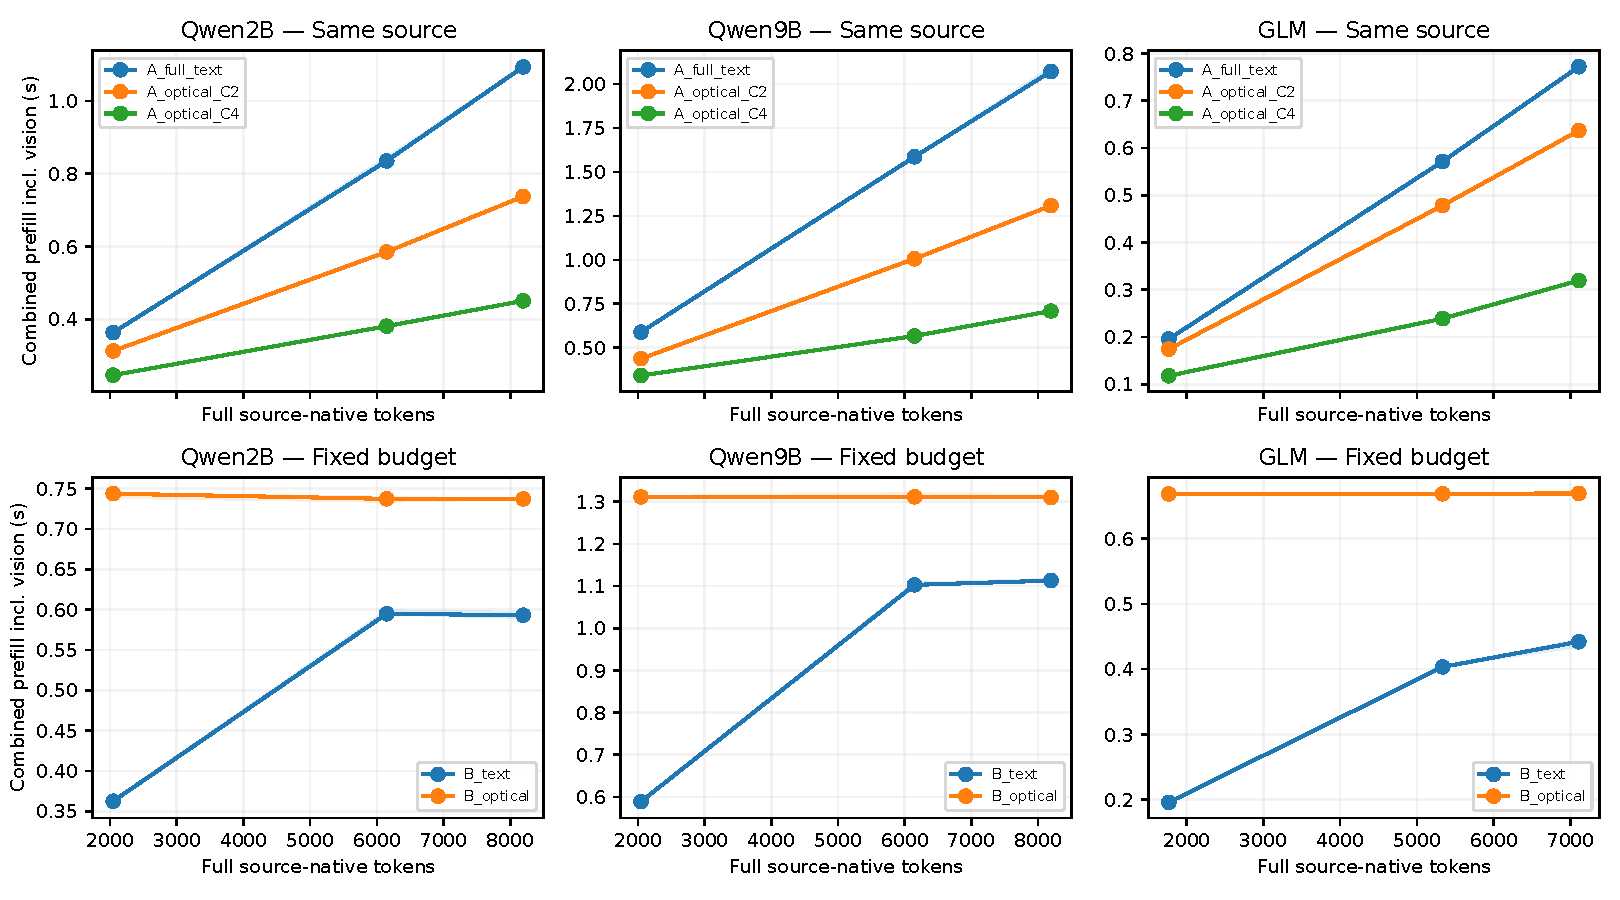
\includegraphics[width=\linewidth]{figures/systems_prefill.pdf}
\caption{Complete original audited combined-prefill profiles, with same-source and fixed-budget views distinguished. Dispersion bands show run IQRs for the predetermined case, not confidence intervals over source documents. Per-reader axes may differ.}
\end{figure}
\begin{figure}[p]\centering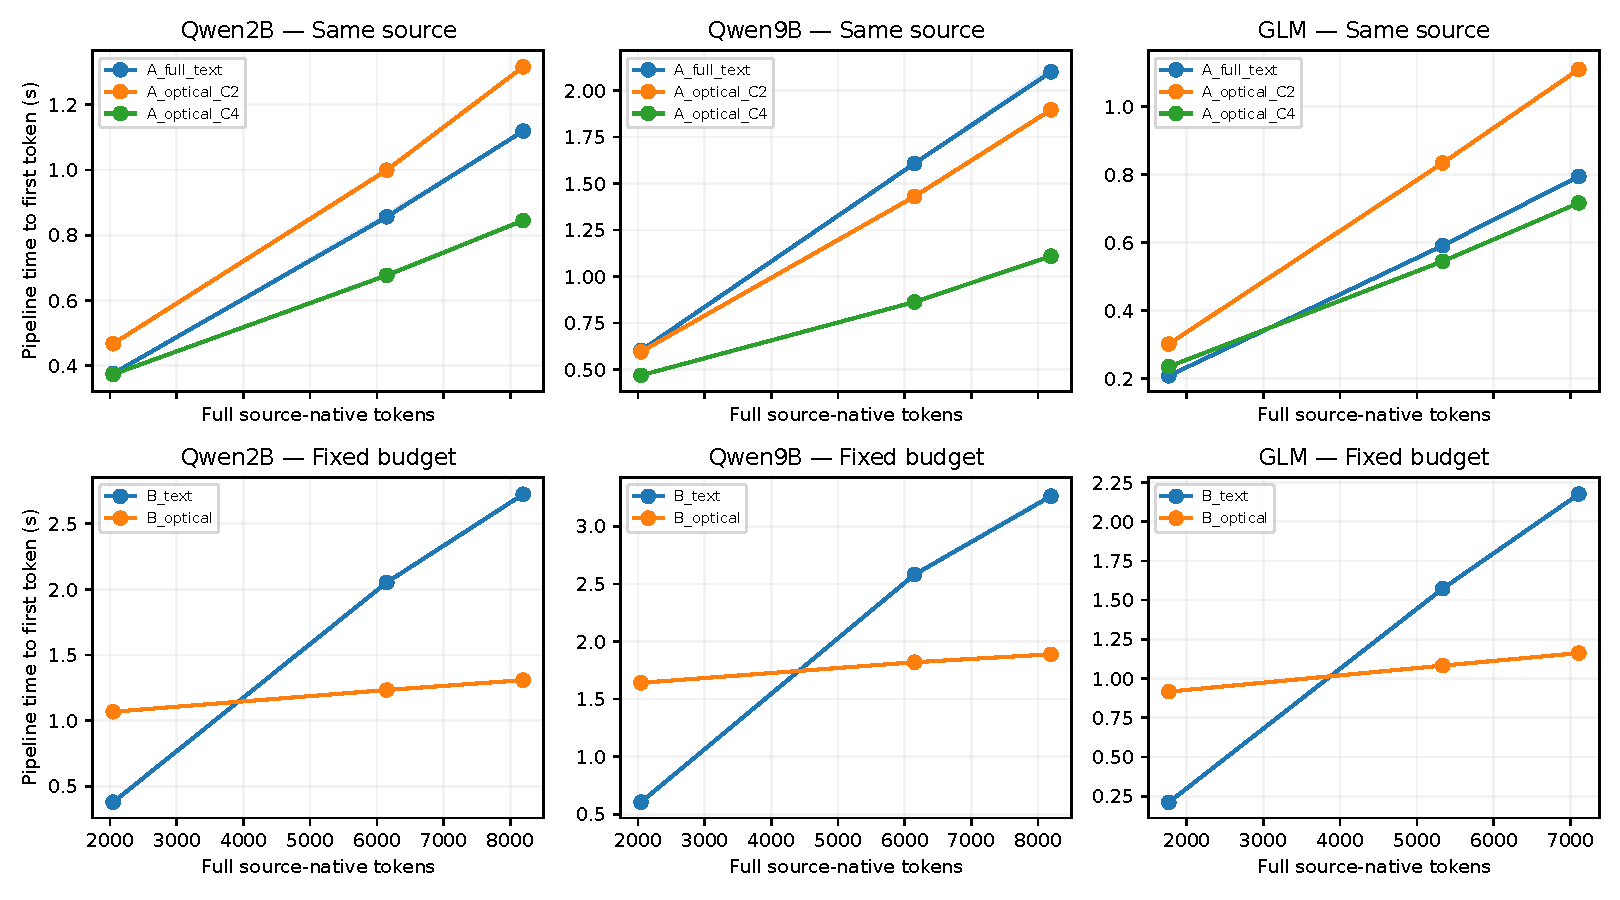
\includegraphics[width=\linewidth]{figures/systems_ttft.pdf}
\caption{Complete original audited pipeline-TTFT profiles. Pipeline TTFT includes representation preparation and processing; optical layout plans are precomputed, while retained-text packing is recomputed. This asymmetry is part of the measured implementation.}
\end{figure}
\begin{figure}[p]\centering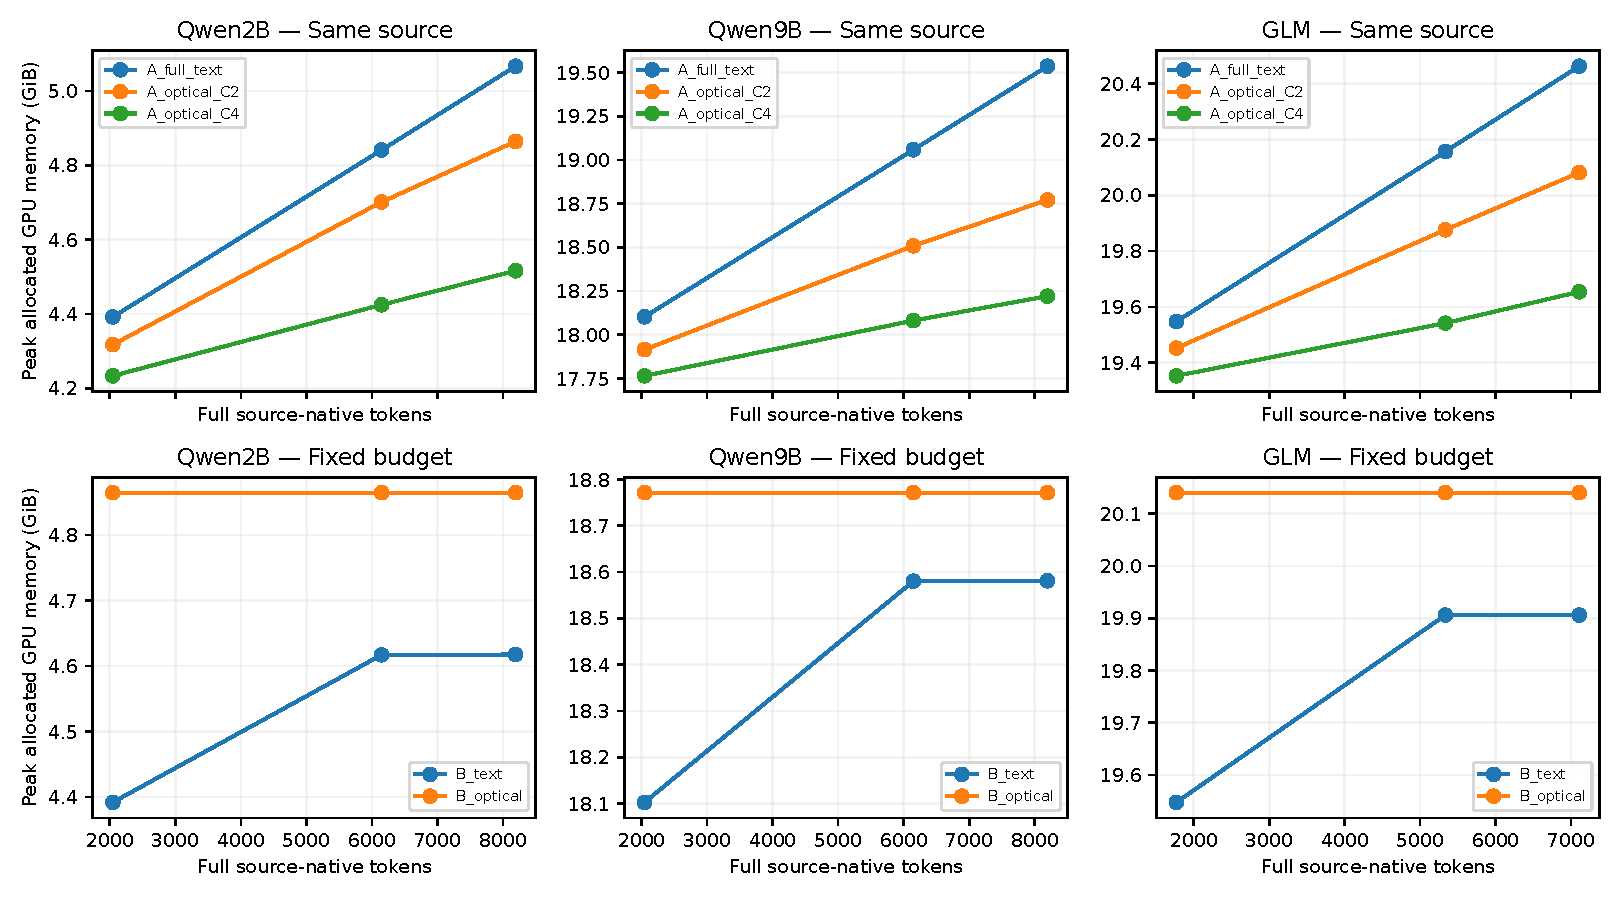
\includegraphics[width=\linewidth]{figures/systems_memory.pdf}
\caption{Complete original audited peak allocated-memory profiles. Resident model allocation is included. Per-panel scales can differ and need not start at zero; numerical differences should guide comparisons.}
\end{figure}
\clearpage

\end{document}
